\PassOptionsToPackage{unicode=true}{hyperref} % options for packages loaded elsewhere
\PassOptionsToPackage{hyphens}{url}
\PassOptionsToPackage{dvipsnames,svgnames*,x11names*}{xcolor}
%
\documentclass[]{krantz}
\usepackage{lmodern}
\usepackage{amssymb,amsmath}
\usepackage{ifxetex,ifluatex}
\usepackage{fixltx2e} % provides \textsubscript
\ifnum 0\ifxetex 1\fi\ifluatex 1\fi=0 % if pdftex
  \usepackage[T1]{fontenc}
  \usepackage[utf8]{inputenc}
  \usepackage{textcomp} % provides euro and other symbols
\else % if luatex or xelatex
  \usepackage{unicode-math}
  \defaultfontfeatures{Ligatures=TeX,Scale=MatchLowercase}
\fi
% use upquote if available, for straight quotes in verbatim environments
\IfFileExists{upquote.sty}{\usepackage{upquote}}{}
% use microtype if available
\IfFileExists{microtype.sty}{%
\usepackage[]{microtype}
\UseMicrotypeSet[protrusion]{basicmath} % disable protrusion for tt fonts
}{}
\IfFileExists{parskip.sty}{%
\usepackage{parskip}
}{% else
\setlength{\parindent}{0pt}
\setlength{\parskip}{6pt plus 2pt minus 1pt}
}
\usepackage{xcolor}
\usepackage{hyperref}
\hypersetup{
            pdftitle={Practical Computing and Bioinformatics for Conservation and Evolutionary Genomics},
            pdfauthor={Eric C. Anderson},
            colorlinks=true,
            linkcolor=Maroon,
            filecolor=Maroon,
            citecolor=Blue,
            urlcolor=Blue,
            breaklinks=true}
\urlstyle{same}  % don't use monospace font for urls
\usepackage{color}
\usepackage{fancyvrb}
\newcommand{\VerbBar}{|}
\newcommand{\VERB}{\Verb[commandchars=\\\{\}]}
\DefineVerbatimEnvironment{Highlighting}{Verbatim}{commandchars=\\\{\}}
% Add ',fontsize=\small' for more characters per line
\usepackage{framed}
\definecolor{shadecolor}{RGB}{248,248,248}
\newenvironment{Shaded}{\begin{snugshade}}{\end{snugshade}}
\newcommand{\AlertTok}[1]{\textcolor[rgb]{0.33,0.33,0.33}{#1}}
\newcommand{\AnnotationTok}[1]{\textcolor[rgb]{0.37,0.37,0.37}{\textbf{\textit{#1}}}}
\newcommand{\AttributeTok}[1]{\textcolor[rgb]{0.61,0.61,0.61}{#1}}
\newcommand{\BaseNTok}[1]{\textcolor[rgb]{0.06,0.06,0.06}{#1}}
\newcommand{\BuiltInTok}[1]{#1}
\newcommand{\CharTok}[1]{\textcolor[rgb]{0.5,0.5,0.5}{#1}}
\newcommand{\CommentTok}[1]{\textcolor[rgb]{0.37,0.37,0.37}{\textit{#1}}}
\newcommand{\CommentVarTok}[1]{\textcolor[rgb]{0.37,0.37,0.37}{\textbf{\textit{#1}}}}
\newcommand{\ConstantTok}[1]{\textcolor[rgb]{0,0,0}{#1}}
\newcommand{\ControlFlowTok}[1]{\textcolor[rgb]{0.27,0.27,0.27}{\textbf{#1}}}
\newcommand{\DataTypeTok}[1]{\textcolor[rgb]{0.27,0.27,0.27}{#1}}
\newcommand{\DecValTok}[1]{\textcolor[rgb]{0.06,0.06,0.06}{#1}}
\newcommand{\DocumentationTok}[1]{\textcolor[rgb]{0.37,0.37,0.37}{\textbf{\textit{#1}}}}
\newcommand{\ErrorTok}[1]{\textcolor[rgb]{0.14,0.14,0.14}{\textbf{#1}}}
\newcommand{\ExtensionTok}[1]{#1}
\newcommand{\FloatTok}[1]{\textcolor[rgb]{0.06,0.06,0.06}{#1}}
\newcommand{\FunctionTok}[1]{\textcolor[rgb]{0,0,0}{#1}}
\newcommand{\ImportTok}[1]{#1}
\newcommand{\InformationTok}[1]{\textcolor[rgb]{0.37,0.37,0.37}{\textbf{\textit{#1}}}}
\newcommand{\KeywordTok}[1]{\textcolor[rgb]{0.27,0.27,0.27}{\textbf{#1}}}
\newcommand{\NormalTok}[1]{#1}
\newcommand{\OperatorTok}[1]{\textcolor[rgb]{0.43,0.43,0.43}{\textbf{#1}}}
\newcommand{\OtherTok}[1]{\textcolor[rgb]{0.37,0.37,0.37}{#1}}
\newcommand{\PreprocessorTok}[1]{\textcolor[rgb]{0.37,0.37,0.37}{\textit{#1}}}
\newcommand{\RegionMarkerTok}[1]{#1}
\newcommand{\SpecialCharTok}[1]{\textcolor[rgb]{0,0,0}{#1}}
\newcommand{\SpecialStringTok}[1]{\textcolor[rgb]{0.5,0.5,0.5}{#1}}
\newcommand{\StringTok}[1]{\textcolor[rgb]{0.5,0.5,0.5}{#1}}
\newcommand{\VariableTok}[1]{\textcolor[rgb]{0,0,0}{#1}}
\newcommand{\VerbatimStringTok}[1]{\textcolor[rgb]{0.5,0.5,0.5}{#1}}
\newcommand{\WarningTok}[1]{\textcolor[rgb]{0.37,0.37,0.37}{\textbf{\textit{#1}}}}
\usepackage{longtable,booktabs}
% Fix footnotes in tables (requires footnote package)
\IfFileExists{footnote.sty}{\usepackage{footnote}\makesavenoteenv{longtable}}{}
\usepackage{graphicx,grffile}
\makeatletter
\def\maxwidth{\ifdim\Gin@nat@width>\linewidth\linewidth\else\Gin@nat@width\fi}
\def\maxheight{\ifdim\Gin@nat@height>\textheight\textheight\else\Gin@nat@height\fi}
\makeatother
% Scale images if necessary, so that they will not overflow the page
% margins by default, and it is still possible to overwrite the defaults
% using explicit options in \includegraphics[width, height, ...]{}
\setkeys{Gin}{width=\maxwidth,height=\maxheight,keepaspectratio}
\setlength{\emergencystretch}{3em}  % prevent overfull lines
\providecommand{\tightlist}{%
  \setlength{\itemsep}{0pt}\setlength{\parskip}{0pt}}
\setcounter{secnumdepth}{5}
% Redefines (sub)paragraphs to behave more like sections
\ifx\paragraph\undefined\else
\let\oldparagraph\paragraph
\renewcommand{\paragraph}[1]{\oldparagraph{#1}\mbox{}}
\fi
\ifx\subparagraph\undefined\else
\let\oldsubparagraph\subparagraph
\renewcommand{\subparagraph}[1]{\oldsubparagraph{#1}\mbox{}}
\fi

% set default figure placement to htbp
\makeatletter
\def\fps@figure{htbp}
\makeatother

\usepackage{booktabs}
\usepackage{longtable}
\usepackage[bf,singlelinecheck=off]{caption}

\usepackage{framed,color}
\definecolor{shadecolor}{RGB}{248,248,248}

\renewcommand{\textfraction}{0.05}
\renewcommand{\topfraction}{0.8}
\renewcommand{\bottomfraction}{0.8}
\renewcommand{\floatpagefraction}{0.75}

\renewenvironment{quote}{\begin{VF}}{\end{VF}}
\let\oldhref\href
\renewcommand{\href}[2]{#2\footnote{\url{#1}}}

\makeatletter
\newenvironment{kframe}{%
\medskip{}
\setlength{\fboxsep}{.8em}
 \def\at@end@of@kframe{}%
 \ifinner\ifhmode%
  \def\at@end@of@kframe{\end{minipage}}%
  \begin{minipage}{\columnwidth}%
 \fi\fi%
 \def\FrameCommand##1{\hskip\@totalleftmargin \hskip-\fboxsep
 \colorbox{shadecolor}{##1}\hskip-\fboxsep
     % There is no \\@totalrightmargin, so:
     \hskip-\linewidth \hskip-\@totalleftmargin \hskip\columnwidth}%
 \MakeFramed {\advance\hsize-\width
   \@totalleftmargin\z@ \linewidth\hsize
   \@setminipage}}%
 {\par\unskip\endMakeFramed%
 \at@end@of@kframe}
\makeatother

\renewenvironment{Shaded}{\begin{kframe}}{\end{kframe}}

\usepackage{makeidx}
\makeindex

\urlstyle{tt}

\usepackage{amsthm}
\makeatletter
\def\thm@space@setup{%
  \thm@preskip=8pt plus 2pt minus 4pt
  \thm@postskip=\thm@preskip
}
\makeatother


% Here is stuff for Rmd notes and cautions and things that ECA lifted from
% Yihui's bookdown book
\makeatletter
\@ifundefined{Shaded}{
}{\renewenvironment{Shaded}{\begin{kframe}}{\end{kframe}}}
\makeatother
\newenvironment{rmdblock}[1]
  {
  \begin{itemize}
  \renewcommand{\labelitemi}{
    \raisebox{-.7\height}[0pt][0pt]{
      {\setkeys{Gin}{width=3em,keepaspectratio}\includegraphics{images/#1}}
    }
  }
  \setlength{\fboxsep}{1em}
  \begin{kframe}
  \item
  }
  {
  \end{kframe}
  \end{itemize}
  }
\newenvironment{rmdnote}
  {\begin{rmdblock}{note}}
  {\end{rmdblock}}
\newenvironment{rmdcaution}
  {\begin{rmdblock}{caution}}
  {\end{rmdblock}}
\newenvironment{rmdimportant}
  {\begin{rmdblock}{important}}
  {\end{rmdblock}}
\newenvironment{rmdtip}
  {\begin{rmdblock}{tip}}
  {\end{rmdblock}}
\newenvironment{rmdwarning}
  {\begin{rmdblock}{warning}}
  {\end{rmdblock}}



\frontmatter
\usepackage[]{natbib}
\bibliographystyle{apalike}

\title{Practical Computing and Bioinformatics for Conservation and Evolutionary Genomics}
\author{Eric C. Anderson}
\date{2020-02-05}

\let\BeginKnitrBlock\begin \let\EndKnitrBlock\end
\begin{document}
\maketitle

% you may need to leave a few empty pages before the dedication page

%\cleardoublepage\newpage\thispagestyle{empty}\null
%\cleardoublepage\newpage\thispagestyle{empty}\null
%\cleardoublepage\newpage
\thispagestyle{empty}

\begin{center}
To my son,

without whom I should have finished this book two years earlier
%\includegraphics{images/dedication.pdf}
\end{center}

\setlength{\abovedisplayskip}{-5pt}
\setlength{\abovedisplayshortskip}{-5pt}

{
\hypersetup{linkcolor=}
\setcounter{tocdepth}{2}
\tableofcontents
}
\listoftables
\listoffigures
\hypertarget{preface}{%
\chapter*{Preface}\label{preface}}


This is a collection of blurbs Eric started writing in the last year to
help remind himself and others of some useful things to know for bioinformatics.

It was started during an extended government shutdown, when it seemed like writing a book
might be in order. Fortunately, the shutdown ended eventually. It is not clear whether a
book will ever come of it, but these notes shall be up on the web indefinitely, so feel free to use
them!

\hypertarget{intro}{%
\chapter{Introduction}\label{intro}}

Nothing here yet.

\hypertarget{erics-notes-of-what-he-might-do}{%
\chapter{Eric's Notes of what he might do}\label{erics-notes-of-what-he-might-do}}

This is where I am going to just throw out ideas and start to organize them. My thought
was that while I am actually doing bioinformatics, etc. in my normal day-to-day work
I will analyze what I am doing and figure out all the different tools that I am using
and organize that or pedagogy.

\begin{itemize}
\tightlist
\item
  Note: I am going to make a companion repository called \texttt{mega-bioinf-pop-gen-examples}
  that will house all of the data sets and things for exercises.
\end{itemize}

\hypertarget{table-of-topics}{%
\section{Table of topics}\label{table-of-topics}}

Man! There is going to be a lot to get through. My current idea
is to meet three times a week. The basic gist of those three sessions
will be like this:

\begin{enumerate}
\def\labelenumi{\arabic{enumi}.}
\item
  \textbf{Fundamental Tools / Environments}: I am thinking 5 weeks on Unix, 1 Week on HPC, 6 Weeks on R/Rstudio, and 3 on Python from within Rstudio (so that students know enough to run python modules like moments.)
\item
  \textbf{Theory and Background}: Population-genetic and bioinformatic theory. Alignment and BW transforms, the coalescent, Fst, etc. Basically things that are needed to understand (to some degree) what various programs/analyses are doing under the hood.
\item
  \textbf{Application and Practice}: Getting the students to get their feet wet and their fingers dirty actually doing it. This time should be entirely practical, with students doing an exercise (in pairs or groups, possibly) with me (or someone else, maybe CH) overseeing.
\end{enumerate}

\begin{longtable}[]{@{}llll@{}}
\toprule
\begin{minipage}[b]{0.10\columnwidth}\raggedright
Week\strut
\end{minipage} & \begin{minipage}[b]{0.21\columnwidth}\raggedright
Fundamental Tools\strut
\end{minipage} & \begin{minipage}[b]{0.29\columnwidth}\raggedright
Theory and Background\strut
\end{minipage} & \begin{minipage}[b]{0.29\columnwidth}\raggedright
Application and Practice\strut
\end{minipage}\tabularnewline
\midrule
\endhead
\begin{minipage}[t]{0.10\columnwidth}\raggedright
1\strut
\end{minipage} & \begin{minipage}[t]{0.21\columnwidth}\raggedright
\emph{Unix Intro}: filesystem; absolute and relative paths, everything is a file; readable, writable, executable; PATH; .bashrc --- hack everyone's to get the time and directory; TAB-completion; \texttt{cd}, \texttt{ls} (colored output), \texttt{cat}, \texttt{head}, \texttt{less}; stdout and stderr and file redirection of either with \texttt{\textgreater{}} and \texttt{2\textgreater{}}; the \texttt{;} vs \texttt{\&}. Using TextWrangler with \texttt{edit} and we need a PC equivalent\ldots{}\strut
\end{minipage} & \begin{minipage}[t]{0.29\columnwidth}\raggedright
\emph{Data Formats}: fasta, fastq, SAM, BAM, VCF, BCF\strut
\end{minipage} & \begin{minipage}[t]{0.29\columnwidth}\raggedright
Command line drills\strut
\end{minipage}\tabularnewline
\begin{minipage}[t]{0.10\columnwidth}\raggedright
2\strut
\end{minipage} & \begin{minipage}[t]{0.21\columnwidth}\raggedright
Programs, binaries, compiling, installing, package management; software distribution; GitHub and sourceforge; admin privileges and sudo, and how you probably won't have that on a cluster.\strut
\end{minipage} & \begin{minipage}[t]{0.29\columnwidth}\raggedright
Fundamental programming concepts; Scripts vs binaries (i.e.~compiled vs interpreted languages); dependencies: headers and libraries; Modularization; Essential algorithms; compression;\strut
\end{minipage} & \begin{minipage}[t]{0.29\columnwidth}\raggedright
samtools, vcftools, bcftools. hands on, doing stuff with them, reading the man pages, exercises.\strut
\end{minipage}\tabularnewline
\begin{minipage}[t]{0.10\columnwidth}\raggedright
3\strut
\end{minipage} & \begin{minipage}[t]{0.21\columnwidth}\raggedright
\emph{Programming on the shell}: variables and variable substitution; Globbing and path expansion; variable modifications; loops; conditionals;\strut
\end{minipage} & \begin{minipage}[t]{0.29\columnwidth}\raggedright
\strut
\end{minipage} & \begin{minipage}[t]{0.29\columnwidth}\raggedright
\strut
\end{minipage}\tabularnewline
\begin{minipage}[t]{0.10\columnwidth}\raggedright
4\strut
\end{minipage} & \begin{minipage}[t]{0.21\columnwidth}\raggedright
\emph{sed, awk, and regular expressions}\strut
\end{minipage} & \begin{minipage}[t]{0.29\columnwidth}\raggedright
\strut
\end{minipage} & \begin{minipage}[t]{0.29\columnwidth}\raggedright
\strut
\end{minipage}\tabularnewline
\begin{minipage}[t]{0.10\columnwidth}\raggedright
5\strut
\end{minipage} & \begin{minipage}[t]{0.21\columnwidth}\raggedright
\emph{HPC}: clusters; nodes; cores; threads. SGE and/or SLURM; \texttt{qsub}; \texttt{qdel}; \texttt{qacct}; \texttt{myjobs}; job arrays.\strut
\end{minipage} & \begin{minipage}[t]{0.29\columnwidth}\raggedright
\strut
\end{minipage} & \begin{minipage}[t]{0.29\columnwidth}\raggedright
\strut
\end{minipage}\tabularnewline
\bottomrule
\end{longtable}

\mainmatter

\hypertarget{part-part-i-essential-computing-skills}{%
\part{Part I: Essential Computing Skills}\label{part-part-i-essential-computing-skills}}

\hypertarget{overview-of-essential-computing-skills}{%
\chapter{Overview of Essential Computing Skills}\label{overview-of-essential-computing-skills}}

What up with this? It appears that bookdown does not let you
write things at the beginning of a Part without putting it under
a chapter heading. Oh well.

\hypertarget{essential-unixlinux-terminal-knowledge}{%
\chapter{Essential Unix/Linux Terminal Knowledge}\label{essential-unixlinux-terminal-knowledge}}

Unix was developed at AT\&T Bell Labs in the 1960s. Formally ``UNIX'' is a
trademarked operating system,
but when most people talk about ``Unix''
they are talking about the \emph{shell}, which is the text-command-driven interface
by which Unix users interact with the computer.

The Unix shell has been around, largely unchanged, for many decades because it is \emph{awesome}.
When you learn it, you aren't learning a fad, but, rather, a mode of interacting
with your computer that has been time tested and will likely
continue to be the lingua franca of large computer systems
for many decades to come.

For bioinformatics, Unix is the tool of choice for a number of reasons: 1) complex analyses
of data can be undertaken with a minimum of words; 2) Unix allows automation of tasks,
especially ones that are repeated many times; 3) the standard set of Unix commands includes
a number of tools for managing large files and for inspecting and manipulating text files; 4) multiple,
successive analyses upon a single stream of data can be expressed and executed efficiently,
typically without the need to write intermediate results to the disk;
5) Unix was developed when computers were extremely limited in terms of memory and speed. Accordingly,
many Unix tools have been well optimized and are appropriate to the massive genomic data sets
that can be taxing even for today's large, high performance computing systems; 6) virtually all state-of-the-art
bioinformatic tools are tailored to run in a Unix environment; and finally, 7) essentially
every high-performance computer cluster runs some variant of Unix, so if you are going to be
using a cluster for your analyses (which is highly likely), then you have gotta know Unix!

\hypertarget{getting-a-bash-shell-on-your-system}{%
\section{Getting a bash shell on your system}\label{getting-a-bash-shell-on-your-system}}

A special part of the Unix operating system is the ``shell.'' This is the system that
interprets commands from the user. At times it behaves like an interpreted programming
language, and it also has a number of features that help to minimize the amount of
typing the user must do to complete any particular tasks. There are a number of
different ``shells'' that people use. We will focus on one called ``bash,'' which stands
for the ``Bourne again shell.'' Many of the shells share a number of features.

Many common operating systems are built upon a Unix or upon Linux---an open-source flavor of
Unix that is, in many scenarios, indistinguishable. Hereafter we will refer
to both Unix and Linux as ``Unix'' systems). For example all Apple Macintosh computers are
built on top of the Berkeley Standard Distribution of Unix and bash is the default
shell. Many people these days
use laptops that run a flavor of Linux like Ubuntu, Debian, or RedHat. Linux
users should ensure that they are running the bash shell. This can be done
by typing ``bash'' at the command line, or inserting that into their profile.
To know what shell is currently running you can type:

\begin{Shaded}
\begin{Highlighting}[]
\BuiltInTok{echo} \VariableTok{$0}
\end{Highlighting}
\end{Shaded}

at the Unix command line. If you are running \texttt{bash} the result should
be

\begin{Shaded}
\begin{Highlighting}[]
\ExtensionTok{-bash}
\end{Highlighting}
\end{Shaded}

PCs running Microsoft Windows are something of the exception in the computer world, in that
they are not running an operating system built on Unix. However, Windows 10 now allows for
a Linux Subsystem to be run. For Windows, it is also possible to install a lightweight
implementation of bash (like Git Bash). This is helpful for learning how to use Unix,
but it should be noted that most bioinformatic tools are still difficult to install
on Windows.

\hypertarget{navigating-the-unix-filesystem}{%
\section{Navigating the Unix filesystem}\label{navigating-the-unix-filesystem}}

Most computer users will be familiar with the idea of saving documents into ``folders.''
These folders are typically navigated using a ``point-and-click'' interface
like that of the Finder in Mac OS X or the File Explorer in a Windows system.
When working in a Unix shell, such a point-and-click interface is typically not available,
and the first hurdle that new Unix users must surmount is learning to quickly navigate in
the Unix filesystem from a terminal prompt. So,
we begin our foray into Unix and its command prompt with this essential skill.

When you start a Unix shell in a terminal window you get a \emph{command prompt}
that might look something like this:

\begin{Shaded}
\begin{Highlighting}[]
\ExtensionTok{my-laptop}\NormalTok{:~ me$}
\end{Highlighting}
\end{Shaded}

or, perhaps something as simple as:

\begin{Shaded}
\begin{Highlighting}[]
\NormalTok{$}
\end{Highlighting}
\end{Shaded}

or maybe something like:

\begin{Shaded}
\begin{Highlighting}[]
\NormalTok{/}\ExtensionTok{~/--%}
\end{Highlighting}
\end{Shaded}

We will adopt the convention in this book that, unless we are intentionally doing something
fancier, the Unix command prompt is given
by a percent sign, and this will be used when displaying text typed at a command
prompt, followed by output from the command. For example

\begin{Shaded}
\begin{Highlighting}[]
\ExtensionTok{%}\NormalTok{ pwd}
\ExtensionTok{/Users/eriq}
\end{Highlighting}
\end{Shaded}

shows that I issued the Unix command \texttt{pwd}, which instructs the computer to
\textbf{p}rint \textbf{w}orking \textbf{d}irectory, and the computer responded by printing
\texttt{/Users/eriq}, which, on my Mac OS X system is my \emph{home directory}.
In Unix parlance, rather than speaking of ``folders,'' we call
them ``directories;'' however, the two are essentially the same thing.
Every user
on a Unix system has a home directory. It is the domain on a shared computer
in which the user has privileges to create and delete files and do work.
It is where most of your work will happen. When you are working in the Unix
shell there is a notion of a
\emph{current working directory}---that is to say, a place within the hierarchy of
directories where you are ``currently working.'' This will become more concrete
after we have encountered a few more concepts.

The specification \texttt{/Users/eriq} is what is known as an \emph{absolute path}, as it provides the
``address'' of my home directory, \texttt{eriq}, on my laptop, starting from the \emph{root}
of the filesystem. Every Unix computer system has a root directory (you can
think of it as the ``top-most'' directory in a hierarchy), and on every Unix system
this root directory always has the special name, \texttt{/}. The address
of a directory relative to the root is specified by starting with the root (\texttt{/})
and then naming each subsequent directory that you must go inside of in order to
get to the destination, each separated by a \texttt{/}. For example, \texttt{/Users/eriq}
tells us that we start at the root (\texttt{/}) and then we go into the \texttt{Users} directory
(\texttt{Users}) and then, from there, into the \texttt{eriq} directory. Note that \texttt{/} is used to mean the root
directory when at the beginning of an absolute path, but in the remainder of the path
its meaning is different: it is used merely as a separator
between directories nested within one another. Figure~\ref{fig:file-hierarchy} shows
an example hierarchy of some of the directories that are found on the author's
laptop.

\begin{figure}

{\centering 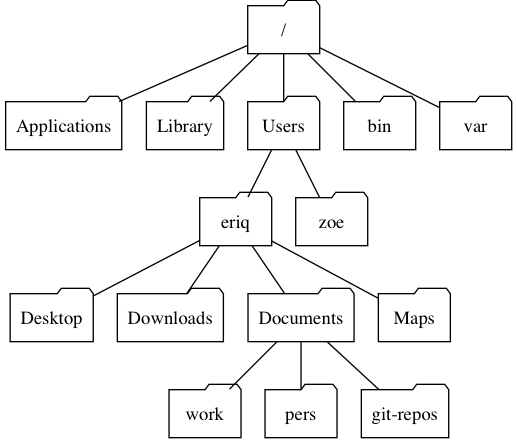
\includegraphics{figs/file-hierarchy} 

}

\caption{A partial view of the directories on the author's laptop.}\label{fig:file-hierarchy}
\end{figure}

From this perspective it is obvious that the directory \texttt{eriq} lives inside \texttt{Users}, and also that, for example,
the absolute path of the directory \texttt{git-repos} would be \texttt{/Users/eriq/Documents/git-repos}.

Absolute paths give the precise location of a directory relative to the root of the filesystem,
but it is not always convenient, nor appropriate, to work entirely with absolute paths.
For one thing, directories that are deeply nested within many others can have long and unwieldy
absolute path names that are hard to type and can be difficult to remember. Furthermore, as we will
see later in this book, absolute paths are typically not \emph{reproducible} from one computer's
filesystem to another. Accordingly, it is more common to give the address of directories using
\emph{relative paths}. Relative paths work much like absolute paths; however, they do not start with
a leading \texttt{/}, and hence they do not take as their
starting point the root directory. Rather, their starting point is implicitly taken
to be the current working directory. Thus, if the current working directory is
\texttt{/Users/eriq}, then the path \texttt{Documents/pers} is a relative path to the
\texttt{pers} directory, as can again be seen in Figure~\ref{fig:file-hierarchy}.

The special relative path symbol \texttt{..} means ``the directory that is one level higher up
in the hierarchy.'' So, if the current working directory were \texttt{/Users/eriq/Documents/git-repos},
then the path \texttt{..} would mean \texttt{/Users/eriq/Documents}, the path
\texttt{../work} gives the directory \texttt{/Users/eriq/Documents/work}, and, by using two or more \texttt{..} symbols
separated by forward slashes, we
can even go up multiple levels in the hierarchy: \texttt{../../../zoe} is a relative path for
\texttt{/Users/zoe}, when the current working directory is \texttt{/Users/eriq/Documents/git-repos}.

When naming paths, another
useful Unix shorthand is \texttt{\textasciitilde{}} (a tilde) which denotes the user's home directory. This is particularly
useful since most of your time in a Unix filesystem will be spent in a directory within your
home directory. Accordingly, \texttt{\textasciitilde{}/Documents/work} is a quick shorthand for
\texttt{/Users/eriq/Documents/work}. This is essential practice if you are working on a large shared computing
resource in which the absolute path to your home directory might be changed by the
system administrator when restructuring the filesystem.

\BeginKnitrBlock{rmdtip}
\textbf{A useful piece of terminology:} in any path, the ``final'' directory
name is called the \emph{basename} of the path. Hence the basename of \texttt{/Users/eriq/Documents/git-repos}
is \texttt{git-repos}. And the basename of \texttt{../../Users} is \texttt{Users}.
\EndKnitrBlock{rmdtip}

\hypertarget{changing-the-working-directory-with-cd}{%
\subsection{\texorpdfstring{Changing the working directory with \texttt{cd}}{Changing the working directory with cd}}\label{changing-the-working-directory-with-cd}}

When you begin a Unix terminal session, the current working
directory is set, by default, to your home directory. However, when you are doing
bioinformatics or otherwise hacking on the command line, you will typically
want to be ``in another directory'' (meaning you will want the current working
directory set to some other directory). For this, Unix provides the \texttt{cd} command, which
stands for \textbf{c}hange \textbf{d}irectory. The syntax is super simple:

cd \emph{path}

where \emph{path} is an absolute or a relative path. For example, to
get to the \texttt{git-repos} directory from my home directory would require
a simple command \texttt{cd\ Documents/git-repos}. Once there, I could change to
my \texttt{Desktop} directory with \texttt{cd\ ../../Desktop}. Witness:

\begin{Shaded}
\begin{Highlighting}[]
\ExtensionTok\NormalTok{ cd Documents/git-repos/}
\ExtensionTok\NormalTok{ cd ../../Desktop}
\ExtensionTok{%}\NormalTok{ pwd}
\ExtensionTok{/Users/eriq/Desktop}
\end{Highlighting}
\end{Shaded}

Once you have used \texttt{cd}, the working directory of your current shell will
remain the same no matter how many other commands you issue,
until you invoke the \texttt{cd} command another time and change
to a different directory.

If you give the \texttt{cd} command with no path specified, your working directory
will be set to your home directory. This is super-handy if you have been
exploring the levels of a Unix filesystem above your home directory and cannot
remember how to get back to your home directory. Just remember that

\begin{Shaded}
\begin{Highlighting}[]
\ExtensionTok{%}\NormalTok{ cd}
\end{Highlighting}
\end{Shaded}

will get you back home.

Another useful shortcut is to supply \texttt{-} (a hyphen) as the path to \texttt{cd}. This will
change the working directory back to where you were before your last invocation
of \texttt{cd}, and it will tell you which directory you have returned to. For example, if you start in \texttt{/Users/eriq/Documents/git-repos} and then
\texttt{cd} to \texttt{/bin}, you can get back to \texttt{git-repos} with \texttt{cd\ -} like so:

\begin{Shaded}
\begin{Highlighting}[]
\ExtensionTok\NormalTok{ cd /bin/}
\ExtensionTok\NormalTok{ cd -}
\ExtensionTok{/Users/eriq/Documents/git-repos}
\ExtensionTok{%}\NormalTok{ pwd}
\ExtensionTok{/Users/eriq/Documents/git-repos}
\end{Highlighting}
\end{Shaded}

Note the output of \texttt{cd\ -} is the newly-returned-to current working directory.

\hypertarget{updating-your-command-prompt}{%
\subsection{Updating your command prompt}\label{updating-your-command-prompt}}

When you are buzzing around in your filesystem, it is often difficult to remember
which directory you are in. You can always type \texttt{pwd} to figure that out,
but the bash shell also provides a way to print the current working directory
\emph{within your command prompt}.

For example, the command:

\begin{Shaded}
\begin{Highlighting}[]
\VariableTok{PS1=}\StringTok{'[\textbackslash{}W]--% '}
\end{Highlighting}
\end{Shaded}

redefines the command prompt to be the basename of the current directory surrounded
by brackets and followed by \texttt{-\/-\%}:

\begin{Shaded}
\begin{Highlighting}[]
\ExtensionTok\NormalTok{ PS1=}\StringTok{'[\textbackslash{}W]--% '}
\NormalTok{[}\ExtensionTok{git-repos}\NormalTok{]--% cd ../}
\NormalTok{[}\ExtensionTok{Documents}\NormalTok{]--% cd ../}
\NormalTok{[}\ExtensionTok{~}\NormalTok{]}\ExtensionTok{--%}\NormalTok{ cd ../}
\NormalTok{[}\ExtensionTok{Users}\NormalTok{]--% }
\end{Highlighting}
\end{Shaded}

This can make it considerably easier to keep track of where you are in your file system.

We will discuss later how to invoke this change automatically in every terminal session
when we talk about customizing environments in Section~\ref{unix-env}.

\hypertarget{tab-completion-for-paths}{%
\subsection{TAB-completion for paths}\label{tab-completion-for-paths}}

Let's be frank\ldots{}typing path names in order to change from one directory to another can feel
awfully tedious, especially when your every neuron is screaming, ``Why can't I just have a friggin' Finder
window to navigate in!'' Do not despair. This is a normal reaction when you first start using Unix.
Fortunately, Unix file-system navigation can be made much less painful (or even enjoyable)
for you by becoming a master of \emph{TAB-completion}. Imagine the Unix shell is watching
your every keystroke and trying to guess what you are about to type. If you type the first part
of a directory name after a command like \texttt{cd} and then hit the TAB key, the shell will respond
with its best guess of how you want to complete what you are typing.

Take the file hierarchy of Figure~\ref{fig:file-hierarchy}, and imagine that we are in the root
directory. At that point, if we type \texttt{cd\ A}, the shell will think "Ooh! I'll bet they want to
change into the directory \texttt{Applications} because that is the only directory that starts with \texttt{A}. Sure enough,
if you hit TAB, the shell adds to the command line so that \texttt{cd\ A} becomes \texttt{cd\ Applications/}
and the cursor is still waiting for further input at the end of the command.
Boom! That was way easier (and more accurate) than typing all those letters after \texttt{A}.

Developing a lightning-fast TAB-completion trigger finger is, quite seriously, essential to surviving and
thriving in Unix. Use your left pinky to hit TAB. Hone your skills. Make sure you can hit TAB with your eyes
closed. TAB early and TAB often!

Once you can hit TAB instantly from within the middle of any phrase, you
will also want to understand a few simple rules of TAB completion:

\begin{enumerate}
\def\labelenumi{\arabic{enumi}.}
\item
  If you try TAB-completing a word on the command line that is not at the beginning
  of the command line (i.e., you are typing a word after a command like \texttt{cd}), then the shell
  tries to complete the word with a \emph{directory name} or a \emph{file name}.
\item
  The shell will only complete an \emph{entire} directory or file name if the name \emph{uniquely} matches the first part of the
  path that has been entered. In our example, there were no other directories than \texttt{Applications} in \texttt{/} that start
  with \texttt{A}, so the shell was certain that we must have been going for \texttt{Applications}.
\item
  If there is more than one directory or file name that matches what you have already typed, then, the first
  time you hit TAB, nothing happens, but the \emph{second} time you hit TAB, the shell will print a list of
  names that match what you have written so far. For example, in our Figure~\ref{fig:file-hierarchy} example,
  hitting TAB after typing \texttt{cd\ \textasciitilde{}/D} does nothing. But the second time we hit TAB we get a list of
  matching names:

\begin{Shaded}
\begin{Highlighting}[]
\ExtensionTok{%}\NormalTok{ cd ~/D}
\ExtensionTok{Desktop/}\NormalTok{  Documents/  Downloads/}
\end{Highlighting}
\end{Shaded}

  So, if we are heading to \texttt{Documents} we can see that adding \texttt{oc} to our command line, to create \texttt{cd\ Doc} would be sufficient to allow the shell to
  uniquely and correctly guess where we are heading. \texttt{cd\ Doc} will TAB-complete into \texttt{cd\ Documents/}
\item
  If there are multiple directory or file names that match the current command line, and they share
  more letters than those currently on the command line, TAB-completion will complete
  the name to the end of the shared portion of the name. An example helps: let's say
  I have the following two directories with hideously long names in my \texttt{Downloads} folder:

\begin{Shaded}
\begin{Highlighting}[]
\ExtensionTok{WIFL.rep_indiv_est.mixture_collection.count.gr8-results}
\ExtensionTok{WIFL.rep_indiv_est.mixture_collection.count-results}
\end{Highlighting}
\end{Shaded}

  Then, TAB completing on \texttt{\textasciitilde{}/Downloads/WIFL.rep} will partially complete so that the prompt and command look like:

\begin{Shaded}
\begin{Highlighting}[]
\ExtensionTok\NormalTok{ cd ~/Downloads/WIFL.rep_indiv_est.mixture_collection.count}
\ExtensionTok{WIFL.rep_indiv_est.mixture_collection.count-results}
\ExtensionTok{WIFL.rep_indiv_est.mixture_collection.count.gr8-results}
\end{Highlighting}
\end{Shaded}

  At this point, adding \texttt{-} and TAB completing will give the first of those directories.
\end{enumerate}

The last example shows just how much typing TAB completion can save you. So, don't be
shy about hitting that TAB key. When navigating your filesystem (or writing longer command
lines that require paths of files) you should consider hitting TAB after every 1 or 2 letters.
In routine work on the command line, probably somewhere around 25\% or more of my keystrokes
are TABs. Furthermore, a TAB is never going to execute a command, and it typically won't
complete to a path that you don't want (unless you got the first part of its name wrong), so there
isn't any risk to hitting TAB all the time.

\hypertarget{listing-the-contents-of-a-directory-with-ls}{%
\subsection{\texorpdfstring{Listing the contents of a directory with \texttt{ls}}{Listing the contents of a directory with ls}}\label{listing-the-contents-of-a-directory-with-ls}}

So far we have been focusing mostly on directories. However, directories themselves
are not particularly interesting---they are merely containers. It is the \emph{files} inside of directories
that we typically work on. The command \texttt{ls} lists the contents---typically files or
other directories---within a directory.

Invoking the \texttt{ls} command without any other arguments (without anything after it)
returns the contents of the current working directory. In our example,
if we are in \texttt{/Users} then we get:

\begin{Shaded}
\begin{Highlighting}[]
\ExtensionTok\NormalTok{ ls}
\ExtensionTok{bam}\NormalTok{                      map-sliced-fastqs-etc.sh}
\ExtensionTok{bam-slices}\NormalTok{               play}
\ExtensionTok{bwa-run-list.txt}\NormalTok{         REDOS-map-sliced-fastqs-etc.sh}
\ExtensionTok{fastq-file-prefixes.txt}\NormalTok{  sliced}
\ExtensionTok{fqslice-22.error}\NormalTok{         slice-fastqs.sh}
\ExtensionTok{fqslice-22.log}\NormalTok{           slicer-lines.txt}
\ExtensionTok{map-etc.sh}\NormalTok{               Slicer-Logs-summary.txt}
\end{Highlighting}
\end{Shaded}

The first line shows the command prompt and the command: \texttt{\%\ ls}, and the remainder is
the output of the command.

Invoked without any further arguments, the \texttt{ls}
command simply lists the contents of the current working directory. However,
you can also direct \texttt{ls} to list the contents of another directory by simply
adding the path (absolute or relative) of that directory on the command line. For example, continuing with
the example in Figure~\ref{fig:file-hierarchy}, when we are in the home directory (\texttt{eriq})
we can see the directories/files
contained within \texttt{Documents} like so:

\begin{Shaded}
\begin{Highlighting}[]
\NormalTok{[}\ExtensionTok{~}\NormalTok{]}\ExtensionTok{--%}\NormalTok{ ls Documents}
\ExtensionTok{git-repos/}\NormalTok{   pers/   work/}
\end{Highlighting}
\end{Shaded}

If you give paths to more than one directory as arguments to \texttt{ls}, then
the contents of each directory are listed after a heading line that gives
the directory's path (as given as an argument to \texttt{ls}), followed by a colon. For example:

\begin{Shaded}
\begin{Highlighting}[]
\NormalTok{[}\ExtensionTok{~}\NormalTok{]}\ExtensionTok{--%}\NormalTok{ ls Documents/git-repos Documents/work}
\ExtensionTok{Documents}\NormalTok{/git-repos:}
\ExtensionTok{ARCHIVED_mega-bioinf-pop-gen.zip}\NormalTok{  lowergranite_0.0.1.tar.gz}
\ExtensionTok{AssignmentAdustment/}\NormalTok{              mega-bioinf-pop-gen-examples/}
\ExtensionTok{CKMRsim/}\NormalTok{                          microhaps_np/}

\ExtensionTok{Documents}\NormalTok{/work:}
\ExtensionTok{assist/}\NormalTok{          maps/            oxford/          uw_days/}
\ExtensionTok{courses_audited/}\NormalTok{ misc/            personnel/}
\end{Highlighting}
\end{Shaded}

You might also note in the above example, that some of the paths listed within
each of the two directories are followed by a slash, \texttt{/}. This \texttt{ls} customization denotes that
they are directories themselves. Much like your command prompt, \texttt{ls} can be customized in ways
that make its output more informative. We will return to that in Section~\ref{unix-env}.

If you pass the path of a file to \texttt{ls}, and that file exists in your filesystem,
then \texttt{ls} will respond by printing the file's path:

\begin{Shaded}
\begin{Highlighting}[]
\ExtensionTok\NormalTok{ ls Documents/try-this-name}
\ExtensionTok{ls}\NormalTok{: Documents/try-this-name: No such file or directory}
\end{Highlighting}
\end{Shaded}

The multi-column, default output of \texttt{ls} is useful when you want
to scan the contents of a directory, and quickly see as many files
as possible in the fewest lines of output.
However, this output format is not well
structured. For example, you don't know how many columns are going to be used in
the default output of \texttt{ls} (that
depends on the length of the filenames and the width of your terminal), and it
offers little information beyond the names of the files.

You can tell the \texttt{ls} command to provide more information, by using it with the \texttt{-l}
option. Appropriately, with the \texttt{-l} option, the \texttt{ls} command will return
output in \emph{long} format:

\begin{Shaded}
\begin{Highlighting}[]
\ExtensionTok{2019-02-08}\NormalTok{ 21:09 /osu-chinook/--% ls -l}
\ExtensionTok{total}\NormalTok{ 108}
\ExtensionTok{drwxr-xr-x}\NormalTok{  2 eriq kruegg  4096 Feb  7 08:26 bam}
\ExtensionTok{drwxr-xr-x}\NormalTok{ 14 eriq kruegg  4096 Feb  8 15:56 bam-slices}
\ExtensionTok{-rw-r--r--}\NormalTok{  1 eriq kruegg 17114 Feb  7 20:16 bwa-run-list.txt}
\ExtensionTok{-rw-r--r--}\NormalTok{  1 eriq kruegg   824 Feb  6 14:14 fastq-file-prefixes.txt}
\ExtensionTok{-rw-r--r--}\NormalTok{  1 eriq kruegg     0 Feb  7 20:14 fqslice-22.error}
\ExtensionTok{-rw-r--r--}\NormalTok{  1 eriq kruegg     0 Feb  7 20:14 fqslice-22.log}
\ExtensionTok{-rwxr--r--}\NormalTok{  1 eriq kruegg  1012 Feb  7 07:59 map-etc.sh}
\ExtensionTok{-rwxr--r--}\NormalTok{  1 eriq kruegg  1138 Feb  7 20:56 map-sliced-fastqs-etc.sh}
\ExtensionTok{drwxr-xr-x}\NormalTok{  3 eriq kruegg  4096 Feb  7 13:01 play}
\ExtensionTok{-rwxr--r--}\NormalTok{  1 eriq kruegg  1157 Feb  8 15:08 REDOS-map-sliced-fastqs-etc.sh}
\ExtensionTok{drwxr-xr-x}\NormalTok{ 14 eriq kruegg  4096 Feb  8 15:49 sliced}
\ExtensionTok{-rwxr--r--}\NormalTok{  1 eriq kruegg   826 Feb  7 20:09 slice-fastqs.sh}
\ExtensionTok{-rw-r--r--}\NormalTok{  1 eriq kruegg  1729 Feb  7 16:11 slicer-lines.txt}
\end{Highlighting}
\end{Shaded}

Each row contains information about only a single file.
The first column indicates what kind of file
each entry is, and also tells us which users have permission to
do certain things with the file (more on this in a few sections).
The third and fourth columns show that the owner of
each file is \texttt{eriq}, who is a user in the group called \texttt{kruegg}. After that
is the size of the file (in bytes) and the date and time it was last modified.

There are a few options to \texttt{ls} that are particularly useful. One is \texttt{-a}, which causes
\texttt{ls} to include in its listing all files, even \emph{hidden} ones. In a Unix file system,
any file whose name starts with a \texttt{.} is considered a \emph{hidden} file. Commonly, such
files are configuration files or other files used by programs that you typically
don't interact with directly. (We will see an example of this when we start working with \texttt{git} for version control, Section~\ref{git-workings}.) The \texttt{-d} option for \texttt{ls} is also'
quite handy. Recall that when you provide the name of a directory as an argument to \texttt{ls},
the default behavior is to list the contents of the directory. This can be troublesome
when you are listing the contents of a subdirectory: \texttt{ls\ \textasciitilde{}/Documents/git-repos/*} lists the
contents (which can be substantial) of each of the directories in my directory, but
I might only want to know the name of each of those directories, rather than their full contents.
\texttt{ls\ -d\ \textasciitilde{}/Documents/git-repos} will do that for you. Finally, the \texttt{-R} option to \texttt{ls} will cause the operating system to drill down, \emph{recursively} into all the subdirectories of the one you
supplied to the command, and list their contents, as well.

\hypertarget{globbing}{%
\subsection{Globbing}\label{globbing}}

If you have ever had to move a large number of files of a certain type from
one folder to another in a Finder window, you know that individually clicking and
selecting each one and then dragging them can be a tedious task (not to mention the disaster
that ensues if you slip on your mouse and end up dropping all the files some place
you did not intend). Unix provides a wonderful system called \emph{filename expansion} or
``globbing'' for quickly providing the names of a large number of files and paths which let's
you operate on multiple files quickly and efficiently. In short, globbing allows for
\emph{wildcard matching} in path names. This means that you can
specify multiple files that have names that share a common part, but differ in other parts.

The most widely used (and the most permissive) wildcard is the asterisk, \texttt{*}. It matches
anything in a file name. So, for example:

\begin{itemize}
\tightlist
\item
  \texttt{*.vcf} will expand to any files in the current directory with the suffix \texttt{.vcf}.
\item
  \texttt{D*s} will expand to any files that start with an uppercase \texttt{D} and end with an \texttt{s}.
\item
  \texttt{*output-*.txt} will expand to any files that include the phrase \texttt{output-} somewhere
  in their name and also end with \texttt{.txt}.
\item
  \texttt{*} will expand to all files in the current working directory.
\item
  \texttt{/usr/local/*/*.sh} will expand to any files ending in \texttt{.sh} that reside within any directory that
  is within the \texttt{/usr/local} directory.
\end{itemize}

\BeginKnitrBlock{rmdnote}
\textbf{Actually, there is some arcana here:} Names of files or directories that start with a
dot (a period) will not expand unless the
dot is included explicitly. Files with names starting with a dot are
``hidden'' files in Unix. You also will not see them in the results of \texttt{ls}, unless you
use the \texttt{-a} option: \texttt{ls\ -a}.
\EndKnitrBlock{rmdnote}

After the asterisk, the next most commonly-used wildcard is the question mark, \texttt{?}. The question mark
denotes any single character in a file name. For example. If you had a series of files that looked
like \texttt{AA-file.txt}, \texttt{AB-file.txt}, \ldots{}, \texttt{AZ-file.txt}. You could get get all those by
using \texttt{A?-file.txt}. This would not expand to, for example, \texttt{AAZ-file.txt}, if that were in the directory.

You can be more specific in globbing by putting things within \texttt{{[}} and \texttt{{]}}. For example:
\texttt{A{[}A-D{]}*} would pick out any files starting with, \texttt{AA}, \texttt{AB}, \texttt{AC}, or \texttt{AD}. Or you could
have said \texttt{A{[}a-d{]}*} which would get any files starting with \texttt{Aa}, \texttt{Ab}, \texttt{Ac}, or \texttt{Ad}. And you
can also do it with numbers: \texttt{{[}0-9{]}}. You can also negate the contents of the \texttt{{[}{]}}, with \texttt{\^{}}. Thus,
\texttt{100\_{[}\^{}ABC{]}*} picks out all files that start with \texttt{100\_} followed by anything that is \emph{not} and \texttt{A}, \texttt{B}, or a \texttt{C}.

Finally, you can be really specific about replacements in file names by iterating over
different possibilities with a comma-separated list within curly braces. For example, \texttt{img.\{png,jpg,svg\}}
will iterate over the values in curly braces and expand to \texttt{img.png\ img.jpg\ img.svg}. Interestingly,
with curly braces, this forms all those file names whether they exist or not. So, unlike \texttt{*} it isn't
really matching available file names.

The last thing to note about all of these globbing constructs is that they are not intimately
associated with the \texttt{ls} command. Rather, they simply provide expansions on the command
line, and the the \texttt{ls} command is listing all those files. For example, try \texttt{echo\ *.txt}.

\hypertarget{what-makes-a-good-file-name}{%
\subsection{What makes a good file-name?}\label{what-makes-a-good-file-name}}

If the foregoing discussion suggests to you that it might not be good to use an
actual \texttt{*}, \texttt{?}, \texttt{{[}}, or \texttt{\{} in names that you give to files and directories
on your Unix system, then congratulations on your intuition! Although you can use
such characters in your filenames, they have to be preceded by a backslash, and it
gets to be a huge hassle. So don't use them in your file names. Additionally,
characters such as \texttt{\#}, \texttt{\textbar{}}, and \texttt{:} do not play well for file names. Don't use them!

Another pet peeve of mine (and anyone who uses Unix) are file names that have spaces in them.
In Windows and on a Mac it is easy to create file names that have spaces in them. In fact, the
standard Windows system comes with such space-containing directory names as \texttt{My\ Documents} or \texttt{My\ Pictures}. Yikes! Please \emph{don't ever do that in your Unix life!} One can deal with spaces in file
names, but there is really no reason to include spaces in your file names, and having spaces in file
names will typically break a good many scripts. Rather than a space, use an underscore, \texttt{\_}, or a
dash, \texttt{-}. You've gotta admit that, not only does \texttt{My-Documents} work better, but it actually
looks better too!

However, should you have to deal with files having spaces in their name, you can
address them by either backslash escaping the spaces, or putting the whole
file name in quotation marks (single or double quotation marks will work).
If you have a file called \texttt{dumb\ file\ name.jpg}, you can address it on the
command line as either of the following three:

\begin{Shaded}
\begin{Highlighting}[]
\ExtensionTok{dumb\textbackslash{} file\textbackslash{} name.jpg}
\StringTok{"dumb file name.jpg"}
\StringTok{'dumb file name.jpg'}
\end{Highlighting}
\end{Shaded}

To make your life easier, however, the bottom line is that you should name your files
on a Unix system using only upper- and lowercase letters (Unix file systems are
case-sensitive), numerals, and the following three punctuation characters: \texttt{.}, \texttt{-}, and \texttt{\_}.
Though you can use other punctuation characters, they often require special treatment, and it
is better to avoid them altogether.

\hypertarget{the-anatomy-of-a-unix-command}{%
\section{The anatomy of a Unix command}\label{the-anatomy-of-a-unix-command}}

Nearly every Unix command that you might invoke follows a certain pattern. First comes
the \texttt{command} itself. This is the word that tells the system the name of the command
that you are actually trying to do. After that, often, you will provide a series
of \emph{options} that will modify the behavior of the command (for example, as we have seen, \texttt{-l}
is an option to the \texttt{ls} command). Finally, you might then provide some \emph{arguments} to the
functions. These are typically paths to files or directories that you would like the
command to operate on. So, in short, a typical Unix command invocation will look
like this:

\texttt{command} \emph{options} \emph{arguments}

Of course, there are exceptions. For example, when invoking Java-based programs from your
shell, arguments might be supplied in ways that make them look like options, etc. But, for
the most part, the above is a useful way of thinking about Unix commands.

Sometimes, especially when using \texttt{samtools} or \texttt{bcftools}, the \texttt{command} part of the
command line might including a command and a subcommand, like \texttt{samtools\ view} or
\texttt{bcftools\ query}. This means that the operating system is calling the program
\texttt{samtools} (for example), and then samtools interprets the next token (\texttt{view}) to
know that it needs to run the \texttt{view} routine, and interpret all following
options in that context.

We will now break down each element in ``\texttt{command} \emph{options} \emph{arguments}''.

\hypertarget{anatomy-command}{%
\subsection{\texorpdfstring{The \texttt{command}}{The command}}\label{anatomy-command}}

When you type a command at the Unix prompt, whether it is a command like \texttt{ls} or
one like \texttt{samtools} (Section \ref{samtools}), the Unix system has to search around
the filesystem for a file that matches the command name and which provides the actual
instructions (the computer code, if you will) for what the command will actually do.
It cannot be stressed enough how important it is to
understand where and how the bash shell searches for these command files. Understanding this
well, and knowing how to add directories that the shell searches for executable
commands will alleviate a lot of frustration that often arises with Unix.

In brief, all Unix shells (and the bash shell specifically) maintain what is called
an \emph{environment variable} called \texttt{PATH} that is a colon-separated list of pathnames
where the shell searches for commands. You can print the \texttt{PATH} variable using
the \texttt{echo} command:

\begin{Shaded}
\begin{Highlighting}[]
\BuiltInTok{echo} \VariableTok{$PATH}
\end{Highlighting}
\end{Shaded}

On a freshly installed system without many customizations the \texttt{PATH} might look like:

\begin{Shaded}
\begin{Highlighting}[]
\ExtensionTok{/usr}\NormalTok{/bin:/bin:}\ExtensionTok{/usr}\NormalTok{/sbin:}\ExtensionTok{/sbin}
\end{Highlighting}
\end{Shaded}

which is telling us that, when bash is searching for a command, it searches for a file
of the same name as the command first in the directory \texttt{/usr/bin}. If it finds it there, then
it uses the contents of that file to invoke the command. If it doesn't find it there,
then it next searches for the file in directory \texttt{/bin}. If it's not there, it searches
in \texttt{/usr/sbin}, and finally in \texttt{/sbin}. If it does not find the command in any of those directories
then it returns the error \texttt{command\ not\ found}.

When you install programs on your own computer system, quite often the installer will modify
a system file that specifies the \texttt{PATH} variable upon startup. Thus after installing some
programs that use the command line on a Mac system, the ``default'' \texttt{PATH} might look like:

\begin{Shaded}
\begin{Highlighting}[]
\ExtensionTok{/usr/local}\NormalTok{/bin:}\ExtensionTok{/usr}\NormalTok{/bin:/bin:}\ExtensionTok{/usr}\NormalTok{/sbin:/sbin:}\ExtensionTok{/opt/X11}\NormalTok{/bin:}\ExtensionTok{/Library/TeX/texbin}
\end{Highlighting}
\end{Shaded}

\hypertarget{the-options}{%
\subsection{\texorpdfstring{The \emph{options}}{The options}}\label{the-options}}

Sometimes these are called flags, and they provide a convenient way of
telling a Unix command how to operate. We have already seen a few of them,
like the \texttt{-a}, \texttt{-l} or \texttt{-d} options to \texttt{ls}.

Most, but not all, Unix tools follow the convention that options specified by a single
letter follow a single dash, while those specified by multiple letters follow two dashes.
Thus, the \texttt{tar} command takes the single character options \texttt{-x}, \texttt{-v}, and \texttt{-f}, but also takes
an option named like \texttt{-\/-check-links}. Some utilities also have two different names---a single-letter
name and a long name---for many options.
For example, the \texttt{bcftools\ view} program uses either \texttt{-a} or \texttt{-\/-trim-alt-alleles} to invoke the option
that trims alternate alleles not seen in a given subset of individuals. Other tools, like BEAGLE, are perfectly
have options that are named with multiple letters following just a single dash.

Sometimes options take parameter values, like \texttt{bcftools\ view\ -g\ het}. In that case, \texttt{het} is
a parameter value. Sometimes the parameter values are added to the option with an equals-sign.

With some unix utilities' single-letter options can be bunged together
following a single dash, like, \texttt{tar\ -xvf} being synonymous with \texttt{tar\ -x\ -v\ -f}. This
is not universal, and it is not recommended to expect it.

Holy Cow! This is not terribly standardized, and probably won't make sense till
you really get in there and starting playing around in Unix\ldots{}

\hypertarget{arguments}{%
\subsection{Arguments}\label{arguments}}

These are often file names, or other things that are not preceded by an option flag.
For example, in the \texttt{ls} command:

\begin{Shaded}
\begin{Highlighting}[]
\FunctionTok{ls}\NormalTok{ -lrt dir3}
\end{Highlighting}
\end{Shaded}

\texttt{-lrt} is giving \texttt{ls} the options \texttt{-l}, \texttt{-r}, and \texttt{-t} and \texttt{dir3} is the \emph{argument}---the
name of the directory whose contents you should list.

\hypertarget{getting-information-about-unix-commands}{%
\subsection{Getting information about Unix commands}\label{getting-information-about-unix-commands}}

Zheesh! The above looks like a horrible mish-mash. How do we find out
how to use/invoke different commands and programs in Unix? Well, most
programs are documented, and you have to learn how to read the documentation.

If a utility is properly installed, you should be able to find its manual page with
the \texttt{man} command. For example, \texttt{man\ ls} or \texttt{man\ tar}. These ``man-pages'', as the
results are called, have a fairly uniform format. They start with a summary of what the
utility does, then then show how it is invoked and what the possible options are by
showing a skeleton in the form:\\
``\texttt{command} \emph{options} \emph{arguments}''\\
and usually square brackets are put around things that are not required. This format
can get quite ugly and hard to parse for an old human brain, like mine, but stick with it.

If you don't have a man-page for a program, you might try invoking the program with
the \texttt{-\/-help} option, or maybe with no option at all.

\hypertarget{handling-manipulating-and-viewing-files-and-streams}{%
\section{Handling, Manipulating, and Viewing files and streams}\label{handling-manipulating-and-viewing-files-and-streams}}

In Unix, there are two main types of files: \emph{regular files} which are things like text files,
figures, etc.---Anything that holds data of some sort. And then there are ``special'' files, which
include \emph{directories} which you've already seen, and \emph{symbolic links} which we will talk about later.

\hypertarget{creating-new-directories}{%
\subsection{Creating new directories}\label{creating-new-directories}}

You can make a new directory with:

\begin{Shaded}
\begin{Highlighting}[]
\FunctionTok{mkdir}\NormalTok{ path}
\end{Highlighting}
\end{Shaded}

where \texttt{path} is a path specification (either absolute or relative). Note that if you
want to make a directory within a subdirectory that does currently not exist, for example:

\begin{Shaded}
\begin{Highlighting}[]
\FunctionTok{mkdir}\NormalTok{ new-dir/under-new-dir}
\end{Highlighting}
\end{Shaded}

when \texttt{new-dir} does not already exist, then you have to either create \texttt{new-dir} first, like:

\begin{Shaded}
\begin{Highlighting}[]
\FunctionTok{mkdir}\NormalTok{ new-dir}
\ExtensionTok{mdkir}\NormalTok{ new-dir/under-new-dir}
\end{Highlighting}
\end{Shaded}

or you have to use the \texttt{-p} option of \texttt{mkdir}, which creates all necessary parent directories
as well, like:

\begin{Shaded}
\begin{Highlighting}[]
\FunctionTok{mkdir}\NormalTok{ -p new-dir/under-new-dir}
\end{Highlighting}
\end{Shaded}

If there is already a file (regular or directory) with the same path specifiation as a directory you are
trying to create, you will get an error from \texttt{mkdir}.

\hypertarget{fundamental-file-handling-commands}{%
\subsection{Fundamental file-handling commands}\label{fundamental-file-handling-commands}}

For the day-to-day business of moving, copying, or removing files in the file system,
the three main Unix commands are:

\begin{itemize}
\tightlist
\item
  \texttt{mv} for moving files and directories
\item
  \texttt{cp} for copying files and directories
\item
  \texttt{rm} for removing files and directories
\end{itemize}

These obviously do different things, but their syntax is somewhat similar.

\hypertarget{mv}{%
\subsubsection{\texorpdfstring{\texttt{mv}}{mv}}\label{mv}}

\texttt{mv} can be invoked with just two arguments like:

\begin{verbatim}
mv this there
\end{verbatim}

which moves the file (or directory) from the path \texttt{this} to the path \texttt{there}.

\begin{itemize}
\tightlist
\item
  If \texttt{this} is a regular file (i.e.~not a directory), and:

  \begin{itemize}
  \tightlist
  \item
    \texttt{there} is a directory,\texttt{this} gets moved inside of \texttt{there}.
  \item
    \texttt{there} is a regular file that exists, then \texttt{there} will get overwritten, becoming a regular
    file that holds the contents of \texttt{this}.
  \item
    \texttt{there} does not exist, it will be created as regular file whose contents are identical
    to those of \texttt{this}.
  \end{itemize}
\item
  If \texttt{this} is a
  directory and:

  \begin{itemize}
  \tightlist
  \item
    \texttt{there} does not exist in the filesystem, the directory \texttt{there} will be made
    and its contents will be the (former) contents of \texttt{this}
  \item
    if \texttt{there} already exists, and is a directory, then the directory \texttt{this} will
    be moved inside of the directory \texttt{there} (i.e.~it will become \texttt{there/this}).
  \item
    if \texttt{there} already exists, but is not a directory, then nothing will change
    in the filesystem, but an an error will
    be reported.
    In all cases, whatever used to exist at path \texttt{this} will no longer be found there.
  \end{itemize}
\end{itemize}

And \texttt{mv} can be invoked with multiple arguments, in which case the last one must be a directory
\emph{that already exists} that receives all the earlier arguments inside it. So, if you already have
a directory named \texttt{dest\_dir} then you can move a lot of things into it like:

\begin{Shaded}
\begin{Highlighting}[]
\FunctionTok{mv}\NormalTok{ file1 file2 dir1 dir2 dest_dir}
\end{Highlighting}
\end{Shaded}

You can also write that as as

\begin{Shaded}
\begin{Highlighting}[]
\FunctionTok{mv}\NormalTok{ file1 file2 dir1 dir2 dest_dir/}
\end{Highlighting}
\end{Shaded}

which makes its meaning a little more clear, but there is no requirement that the
final argument have a trailing \texttt{/}.

Note, if any files in \texttt{dest\_dir} have the same name as the files you are moving into
\texttt{dest\_dir} they \emph{will} get overwritten.

So, you have gotta be careful not to overwrite stuff that you don't want to overwrite.

\hypertarget{cp}{%
\subsubsection{\texorpdfstring{\texttt{cp}}{cp}}\label{cp}}

This works much the same way as \texttt{mv} with two different flavors:

\begin{Shaded}
\begin{Highlighting}[]
\FunctionTok{cp}\NormalTok{ this there}
\end{Highlighting}
\end{Shaded}

and

\begin{Shaded}
\begin{Highlighting}[]
\FunctionTok{cp}\NormalTok{ file1 file2 dest_dir}
\CommentTok{# or}
\FunctionTok{cp}\NormalTok{ file1 file2 dest_dir/}
\end{Highlighting}
\end{Shaded}

The result is very much like that of \texttt{mv}, but instead of moving the file
from one place to another (an operation that can actually be done without moving the
data within the file to a different place on the hard drive), the \texttt{cp} command actually
makes a full copy of files. Note that, if the files are large, this can take a long time.

\hypertarget{rm}{%
\subsubsection{\texorpdfstring{\texttt{rm}}{rm}}\label{rm}}

Finally we get to the very spooky \texttt{rm} command, which is short for ``remove.'' If you
say ``rm myfile.txt'' the OS will remove that file from your hard drive's directory. The data
that were in the file might live on for some time on your hard drive---in other words, by default,
\texttt{rm} does not wipe the file off your hard drive, but simply ``forgets'' where to look for that file. And
the space that file took up on your hard drive is no longer reserved, and could easily be
overwritten the next time you write something to disk. (Nonetheless, if you do \texttt{rm} a file, you should never expect to be able to get it back). So, be very careful about using \texttt{rm}. It takes an \texttt{-r} option for recursively removing directories \emph{and} all of
their contents.

When used in conjunction with globbing, \texttt{rm} can be very useful. For example, if you wanted
to remove all the files in a directory with a \texttt{.jpg} extension, you would do \texttt{rm\ *.jpg} from
within that directory. However, it's a disaster to accidentally remove a number of files you
might not have wanted to. So, especially as you are getting familiar with Unix, it is
worth it to experiment with your globbing using \texttt{ls} first, to see what the results are,
and only when you are convinced that you won't remove any files you really want should you
end up using \texttt{rm} to remove those files.

\hypertarget{viewing-files}{%
\subsection{``Viewing'' Files}\label{viewing-files}}

In a typical GUI-based environment, when you interact with files on your computer,
you typically open the files with some application. For example, you open Word files
with Microsoft Word. When working on the Unix shell, that same paradigm does not
really exist. Rather, (apart from a few cases like the text editors, \texttt{nano}, \texttt{vim} and
\texttt{emacs}, instead of opening a file and letting the user interact with it the shell is
much happier just streaming the contents of the file to the terminal.

The most basic of such commands is the \texttt{cat} command, which \emph{catenates} the contents
of a file into a very special \emph{data stream} called \emph{stdout}, which is short
for ``standard output.'' If you don't provide any other instruction, data that gets
streamed to \emph{stdout} just shoots by on your terminal screen. If the file is very large, it might
do this for a long time. If the file is a \emph{text file} then the data in it can be
written out in letters that are recognizable. If it is a \emph{binary file} then there is
no good way to represent the contents as text letters, and your screen will be filled with
all sorts of crazy looking characters.

It is generally best not to \texttt{cat} very large files, especially binary ones. If you do and
you need to stop the command from continuing to spew stuff across your screen, you can type
\texttt{cntrl-c} which is the universal Unix command for ``kill the current process happening on the
shell.'' Usually that will stop it.

\BeginKnitrBlock{rmdtip}
\textbf{A note regarding terminals:} On a Mac, the Terminal app is quite fast at spewing text
across the screen. Megabytes of text or binary gibberish can flash by in seconds flat. This
is not the case with the terminal window within RStudio, which can by abysmally slow, and usually
doesn't store many lines of output.
\EndKnitrBlock{rmdtip}

Sometimes you want to just look at the top of a file. The \texttt{head} command
shows you the first 10 lines of a file. That is valuable. The \texttt{less} command
shows a file one screenful at a time. You can hit the space bar to see the next screenful,
and you can hit \texttt{q} to quit viewing the file.

Try navigating to a file and using \texttt{cat}, \texttt{head}, and \texttt{less} on it.

One particularly cool thing about \texttt{cat} is that if you say

\begin{Shaded}
\begin{Highlighting}[]
\FunctionTok{cat}\NormalTok{ file1 file2}
\end{Highlighting}
\end{Shaded}

it will catenate the contents of both files, in order, to \emph{stdout}.

Now, one Big Important Unix fact is that many programs written to run in the
Unix shell behave in the same way regarding their output: they write their
output to \emph{stdout}. We have already seen this with \texttt{ls}: its output just
gets written to the screen, which is where \emph{stdout} goes by default.

\hypertarget{redirecting-standard-output-and}{%
\subsection{\texorpdfstring{Redirecting standard output: \texttt{\textgreater{}} and \texttt{\textgreater{}\textgreater{}}}{Redirecting standard output: \textgreater{} and \textgreater{}\textgreater{}}}\label{redirecting-standard-output-and}}

Unix starts to get really fun when you realize that you can ``redirect'' the
contents of \emph{stdout} from any command (or group of commands\ldots{}see the next chapter!)
to a file. To do that, you merely follow the command (and all its options and arguments)
with \texttt{\textgreater{}\ path} where \texttt{path} is the path specifying the file into which you
wish to redirect \emph{stdout}.

Witness, try this:

\begin{Shaded}
\begin{Highlighting}[]
\CommentTok{# echo three lines of text to a file in the /tmp directory}
\BuiltInTok{echo} \StringTok{"bing}
\StringTok{bong}
\StringTok{boing"} \OperatorTok{>}\NormalTok{ /tmp/file1}

\CommentTok{# echo three more lines of text to another file}
\BuiltInTok{echo} \StringTok{"foo}
\StringTok{bar}
\StringTok{baz"} \OperatorTok{>}\NormalTok{ /tmp/file2}

\CommentTok{# now view the contents of the first file}
\FunctionTok{cat}\NormalTok{ /tmp/file1}

\CommentTok{# and the second file:}
\FunctionTok{cat}\NormalTok{ /tmp/file2}
\end{Highlighting}
\end{Shaded}

It is important to realize that when you redirect output into a file
with \texttt{\textgreater{}}, any contents that previously existed in that file will
be deleted (wiped out!). So be careful about redirecting. Don't
accidentally redirect output into a file that has valuable data in it.

The \texttt{\textgreater{}\textgreater{}} redirection operator does not delete the destination file before
it redirects output into it. Rather, \texttt{\textgreater{}\textgreater{}\ file} means ``append \emph{stdout} to the contents that already exist in \texttt{file}.'' This can be very useful
sometimes.

\hypertarget{stdin-and}{%
\subsection{\texorpdfstring{stdin, \texttt{\textless{}} and \texttt{\textbar{}}}{stdin, \textless{} and \textbar{}}}\label{stdin-and}}

Not only do most Unix-based programs deliver output to standard output, but
most utilities can also receive input from a file stream called \emph{stdin} which
is short for ``standard input.''

If you have data in a file that you want to send into standard input
for a utility, you can use the \texttt{\textless{}} like this:

\begin{Shaded}
\begin{Highlighting}[]
\BuiltInTok{command} \OperatorTok{<}\NormalTok{ file}
\end{Highlighting}
\end{Shaded}

But, since most Unix utilities also let you specify the file as an argument,
this is not used very much.

However, what is used all the time in Unix, and it is one of the things
that makes it super fun, is the pipe, \texttt{\textbar{}}, which says, "take \emph{stdout} coming
out of the command on the left and redirect it into \emph{stdin} going into
the command on the right of the pipe.

For example, if I wanted to count the number of files and directories stored in my \texttt{git-repos}
directory, I could do

\begin{Shaded}
\begin{Highlighting}[]
\ExtensionTok{%}\NormalTok{ ls -dl Documents/git-repos/* }\KeywordTok{|} \FunctionTok{wc} 
     \ExtensionTok{174}\NormalTok{    1566   14657}
\end{Highlighting}
\end{Shaded}

which pipes the output of \texttt{ls\ -dl} (one line per file) into the \emph{stdin} for the \texttt{wc} command, which
counts the number of lines, words, and letters sent to its standard input. So, the output tells
me that there are 174 files and directories in my directory \texttt{Documents/git-repos}.

Note that pipes and redirects can be combined in sequence over multiple
operations or commands. This is what gives rise to the terminology of
making ``Unix pipelines:'' the data are like streams of water coming into
or out of different commands, and the pipes hook up all those streams into
a pipeline.

\hypertarget{stderr}{%
\subsection{stderr}\label{stderr}}

While output from Unix commands is often written to \emph{stdout}, if anything goes wrong with
a program, then messages about that get written to a different stream called \emph{stderr}, which, you
guessed it! is short for ``standard error''. By default, both \emph{stdout} and \emph{stderr} get written
to the terminal, which is why it can be hard for beginners to think of them as separate streams.\\
But, indeed, they are. Redirecting \emph{stdout} with \texttt{\textgreater{}}, that does \textbf{not} redirect \emph{stderr}.

For example. See what happens when we ask \texttt{ls} to list a file that does not exist:

\begin{Shaded}
\begin{Highlighting}[]
\NormalTok{[}\ExtensionTok{~}\NormalTok{]}\ExtensionTok{--%}\NormalTok{ ls file-not-here.txt }
\ExtensionTok{ls}\NormalTok{: file-not-here.txt: No such file or directory}
\end{Highlighting}
\end{Shaded}

The error message comes back to the screen. If you redirect the output
it still comes back to the screen!

\begin{Shaded}
\begin{Highlighting}[]
\NormalTok{[}\ExtensionTok{~}\NormalTok{]}\ExtensionTok{--%}\NormalTok{ ls file-not-here.txt }\OperatorTok{>}\NormalTok{ out.txt }
\ExtensionTok{ls}\NormalTok{: file-not-here.txt: No such file or directory}
\end{Highlighting}
\end{Shaded}

If you want to redirect \emph{stderr}, then you need to specify which stream
it is. On all Unix systems, \emph{stderr} is stream \#2, so the \texttt{2\textgreater{}} syntax can be
used:

\begin{Shaded}
\begin{Highlighting}[]
\NormalTok{[}\ExtensionTok{~}\NormalTok{]}\ExtensionTok{--%}\NormalTok{ ls file-not-here.txt }\OperatorTok{2>}\NormalTok{ out.txt }
\end{Highlighting}
\end{Shaded}

Then there is no output of \emph{stderr} to the terminal, and when you \texttt{cat} the output
file, you see that it went there!

\begin{Shaded}
\begin{Highlighting}[]
\NormalTok{[}\ExtensionTok{~}\NormalTok{]}\ExtensionTok{--%}\NormalTok{ cat out.txt }
\ExtensionTok{ls}\NormalTok{: file-not-here.txt: No such file or directory}
\end{Highlighting}
\end{Shaded}

Doing bioinformatics, you will find that there will be failures of various programs.
It is essential when you write bioinformatic pipelines to redirect \emph{stderr} to a
file so that you can go back, after the fact, to sleuth out why the failure occurred.
Additionally, some bioinformatic programs write things like progress messages to
\emph{stderr} so it is important to know how to redirect those as well.

\hypertarget{symbolic-links}{%
\subsection{Symbolic links}\label{symbolic-links}}

Besides regular files and directories, a third type of file in Unix is called a
\emph{symbolic link}. It is a special type of file whose contents are just an
absolute or a relative path to another file. You can think of symbolic links
as ``shortcuts'' to different locations in your file system. There are many
useful applications of symbolic links.

Symbolic links are made using the \texttt{ln} command with the \texttt{-s} option. For example,
if I did this in my home directory:

\begin{Shaded}
\begin{Highlighting}[]
\NormalTok{[}\ExtensionTok{~}\NormalTok{]}\ExtensionTok{--%}\NormalTok{ ln -s /Users/eriq/Documents/git-repos/srsStuff srs}
\end{Highlighting}
\end{Shaded}

then \texttt{srs} becomes a file whose full listing (from \texttt{ls\ -l\ srs}) looks like:

\begin{Shaded}
\begin{Highlighting}[]
\ExtensionTok{lrwxrwxr-x}\NormalTok{  1 eriq  staff    40B Jan  9 19:24 srs@ -}\OperatorTok{>}\NormalTok{ /Users/eriq/Documents/git-repos/srsStuff}
\end{Highlighting}
\end{Shaded}

\hypertarget{file-permissions}{%
\subsection{File Permissions}\label{file-permissions}}

Unix systems often host many different users. Some users might belong to the
same research group, and might like to be able to read the files (and/or use
the programs) that their colleagues have in their accounts.

The Unix file system uses a system of permissions that gives rights to various
classes of users to read, write, or execute files. The permissions associated with
a file can be viewed using \texttt{ls\ -l}. They are captured in the first column which might
look something like \texttt{-rwxr-xr-x}. When you first start looking at these, they can
be distressingly difficult to visually parse. But you will get better at it! Let's
start breaking it down now.

The file description string, in a standard Unix setting, consists of 10 characters.

\begin{itemize}
\tightlist
\item
  The first tells what kind of file it is: \texttt{-} = regular file, \texttt{d} = directory, \texttt{l} = symbolic link.
\item
  The next group of three characters denote whether the owner/user of the file has
  permission to either read, write, or execute the file.\\
\item
  The following two groups of three characters are the same thing for users within the
  users group, and for all other users, respectively.
\end{itemize}

Here is a figure from \href{https://unix.stackexchange.com/questions/183994/understanding-unix-permissions-and-file-types}{the web} that we can talk about:
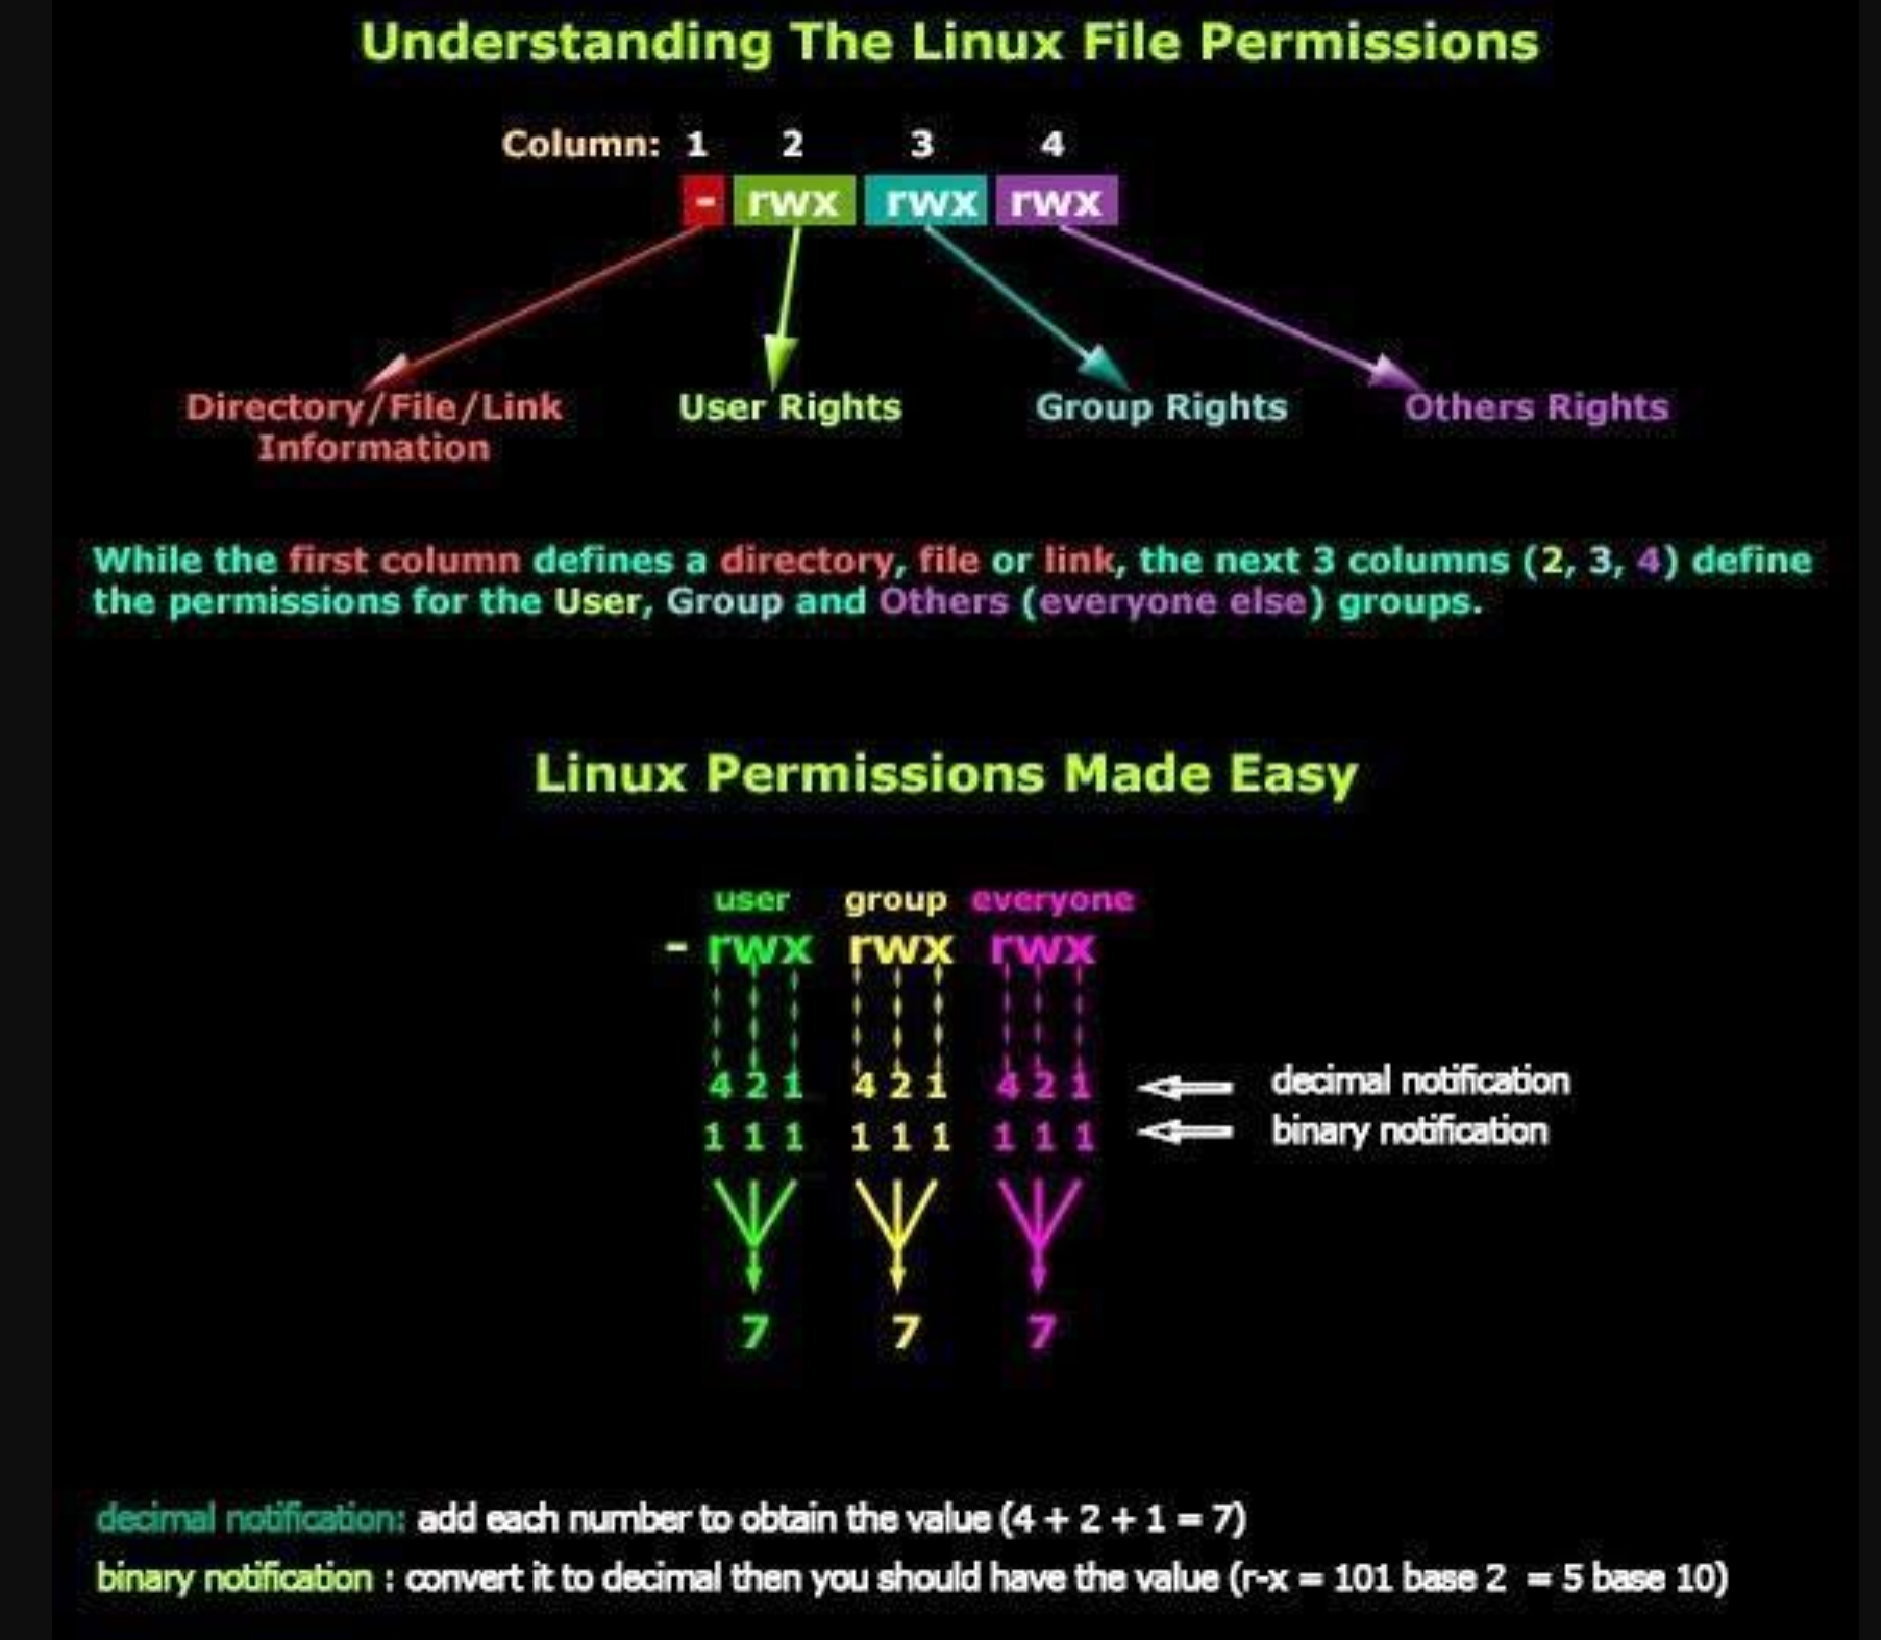
\includegraphics{figs/permissions.pdf}

Permissions can be changed with the \texttt{chmod} command. We will talk in class about
how to use it with the octal representation of permissions.

\hypertarget{editing-text-files-at-the-terminal}{%
\subsection{Editing text files at the terminal}\label{editing-text-files-at-the-terminal}}

Sometimes you might need to edit text files at the command line.

The easiest text editor to use on the command line is \texttt{nano}.
Try typing \texttt{nano\ a-file.txt} and type a few things. It is
pretty self explanatory.

\hypertarget{unix-env}{%
\section{Customizing your Environment}\label{unix-env}}

Previously we saw how to modify your command prompt to tell you what the current
working directory is (remember \texttt{PS1=\textquotesingle{}{[}\textbackslash{}W{]}-\/-\%\ \textquotesingle{}}). The limitation of giving that
command on the command line is that if you logout and then log back in again, or open
a new Terminal window, you will have to reissue that command in order to achieve
the desired look of your command prompt. Quite often a Unix user would like to make
a number of customization to the look, feel, and behavior of their Unix shell.
The bash shell allows these customization to be specified in two different files that
are read by the system so as to invoke the customization. The two files are hidden files
in the home directory: \texttt{\textasciitilde{}/.bashrc} and \texttt{\textasciitilde{}/.bash\_profile}. They are used by the Unix system
in two slightly different contexts, but for most purposes, you, the user, will not need or
even want to distinguish between the different contexts. Managing two separate files
of customization is unnecessary and requires duplication of your efforts, and can lead to inconsistent
and confusing results, so here is what we will do:

\begin{enumerate}
\def\labelenumi{\arabic{enumi}.}
\tightlist
\item
  Keep all of our customization in \texttt{\textasciitilde{}/.bashrc}.
\item
  Insert commands in \texttt{\textasciitilde{}/.bash\_profile} that say, "Hey computer! If you are looking
  for customization in here, don't bother, just get them straight out of \texttt{\textasciitilde{}/.bashrc}.
\end{enumerate}

We take care of \#2, by creating the file \texttt{\textasciitilde{}/.bash\_profile} to have the following
lines in it:

\begin{Shaded}
\begin{Highlighting}[]

\KeywordTok{if}\BuiltInTok{ [} \OtherTok{-f}\NormalTok{ ~/.bashrc}\BuiltInTok{ ]}\NormalTok{; }\KeywordTok{then}
    \BuiltInTok{source}\NormalTok{ ~/.bashrc}
\KeywordTok{fi}
\end{Highlighting}
\end{Shaded}

Taking care of \#1 is now just a matter of writing commands into \texttt{\textasciitilde{}/.bashrc}. In the following
are some recommended customization.

\hypertarget{appearances-matter}{%
\subsection{Appearances matter}\label{appearances-matter}}

Some customization just change the way your shell looks or what type of output
is given from different commands. Here are some lines to add to your \texttt{\textasciitilde{}/.bashrc}
along with some discussion of each.

\begin{Shaded}
\begin{Highlighting}[]
\BuiltInTok{export} \VariableTok{PS1=}\StringTok{'[\textbackslash{}W]--% '}
\end{Highlighting}
\end{Shaded}

This gives a tidier and more informative command prompt. The \texttt{export} command before
it tells the system to pass the value of this \emph{environment variable}, \texttt{PS1}, along
to any other shells that get spawned by the current one.

\begin{Shaded}
\begin{Highlighting}[]
\BuiltInTok{alias}\NormalTok{ ls=}\StringTok{'ls -GFh'}
\end{Highlighting}
\end{Shaded}

This makes it so that each time you invoke the \texttt{ls} command, you do so with the
options \texttt{-G}, \texttt{-F}, and \texttt{-h}. To find out on your own what those options do, you can
type \texttt{man\ ls} at the command line and read the output, but briefly: \texttt{-G} causes directories and
different file types to be printed in different colors, \texttt{-F} causes a \texttt{/} to be printed after
directory names, and other characters to be printed at the end of the names of different
file types, and \texttt{-h} causes file sizes to be printed in an easily human-readable form when
using the \texttt{-l} option.

\hypertarget{where-are-my-programscommands-at}{%
\subsection{Where are my programs/commands at?!}\label{where-are-my-programscommands-at}}

We saw in Section \ref{anatomy-command} that bash searches the directories listed in the
\texttt{PATH} variable to find commands and executables. You can modify the PATH variable to include
directories where you have installed different programs. In doing so, you want to make sure
that you don't lose any of the other directories in \texttt{PATH}, so there is a certain way to
go about redefining \texttt{PATH}. If you want to add the path \texttt{/a-new/program/directory} to your
PATH variable you do it like this:

\begin{Shaded}
\begin{Highlighting}[]
\VariableTok{PATH=$PATH}\NormalTok{:/a-new/program/directory}
\end{Highlighting}
\end{Shaded}

\hypertarget{a-few-more-important-keystrokes}{%
\section{A Few More Important Keystrokes}\label{a-few-more-important-keystrokes}}

If a command ``gets stuck'' or is running longer than it should be, you can usually
kill/quit it by doing \texttt{cntrl-c}.

Once you have given a command, it gets stored in your bash history. You can use the
up-arrow key to cycle backward through different commands in your history. This is particularly
useful if you are building up complex pipelines on the command line piece by piece, looking at
the output of each to make sure it is correct. Rather than re-typing what you did for the last
command line, you just up-arrow it.

Once you have done an up-arrow or two, you can cycle back down through your history with
a down-arrow.

Finally, you can search through your bash history by typing \texttt{cntrl-r} and then typing
the word/command you are looking for. For example, if, 100 command lines back, you
used a command that involved the program \texttt{awk}, you can search for that by typing
\texttt{cntrl-r} and then typing \texttt{awk}.

One last big thing to note: the \texttt{\#} is considered a \emph{comment character} in bash.
This means that any text following a \texttt{\#} (unless it is backslash-escaped or inside quotation marks),
until the next line ending,
will be ignored by the shell.

\hypertarget{a-short-list-of-additional-useful-commands.}{%
\section{A short list of additional useful commands.}\label{a-short-list-of-additional-useful-commands.}}

Everyone should be familiar with the following commands, and the
options that follow them on each line below. One might even think of
scanning the manual page for each of these:

\begin{itemize}
\tightlist
\item
  \texttt{echo}
\item
  \texttt{cat}
\item
  \texttt{head}, \texttt{-n,\ -c}
\item
  \texttt{tail}, \texttt{-n}
\item
  \texttt{less}
\item
  \texttt{sort}, \texttt{-n\ -b\ -k}
\item
  \texttt{paste}
\item
  \texttt{cut}, \texttt{-d}
\item
  \texttt{tar}, \texttt{-cvf,\ -xvf}
\item
  \texttt{gzip}, \texttt{-c}
\item
  \texttt{du}, \texttt{-h\ -C},
\item
  \texttt{wc}
\item
  \texttt{date}
\item
  \texttt{uniq}
\item
  \texttt{chmod}, \texttt{u+x}, \texttt{ug+x}
\item
  \texttt{grep}
\end{itemize}

\hypertarget{two-important-computing-concepts}{%
\section{Two important computing concepts}\label{two-important-computing-concepts}}

\hypertarget{compression}{%
\subsection{Compression}\label{compression}}

Most file storage types (like text files) are a bit wasteful in terms of
file space: every character in a text file takes the same number of bytes to
store, whether it is a character that is used a lot, like \texttt{s} or \texttt{e}, or whether
it is a character that is seldom seen in many text files, like \texttt{\^{}}. \emph{Compression}
is the art of creating a code for different types of data that uses fewer bits to
encode ``letters'' (or ``chunks'' of data) that occur frequently and it reserves codewords of
more bits to encode less frequently occurring chunks in the data. The result is that the
total file size is smaller than the uncompressed version. However, in order to read it,
the file must be decompressed.

In bioinformatics, many of the files you deal with will be compressed, because that
can save many terabytes of disk space. Most often, files will be compressed using the
\texttt{gzip} utility, and they can be uncompressed with the \texttt{gunzip} command. Sometimes
you might want to just look at the fist part of a compressed file. If the file is compressed
with \texttt{gzip}, you can decompress to \emph{stdout} by using \texttt{gzcat} and then pipe it to \texttt{head}, for example.

A central form of compression in bioinformatics is called \texttt{bgzip} compression
which compresses files into a series of blocks of the same size, situated in such a way that
it is possible to \emph{index} the contents of the file so that certain parts of the file can be
accessed without decompressing the whole thing. We will encounter indexed compressed files a
lot when we start dealing with BAM and vcf.gz files.

\hypertarget{hashing}{%
\subsection{Hashing}\label{hashing}}

The final topic we will cover here is the topic of hashing, an in particular
the idea of ``fingerprinting'' files on ones computer. This process is central
to how the git version control system works, and it is well worth knowing about.

Any file on your computer can be thought of as a series of bits, 0's and 1's, as,
fundamentally, that is what the file is. A \emph{hashing algorithm} is an algorithm
that maps a series of bits (or arbitrary length) to a short sequence of bits. The
SHA1 hashing algorithm maps arbitrary sequences of bits to a sequence of 160 bits.

There are \(2^{160} \approx 1.46 \times 10^{48}\) possible bit sequences of length 160.
That is a vast number. If your hashing algorithm is well randomized, so that bit sequences
are hashed into 160 bits in a roughly uniform distribution, then it is exceedingly unlikely
that any two bit sequences (i.e.~files on your filesystem) will have the same hash (``fingerprint'')
unless they are perfectly identical. As hashing algorithms are often quite fast to compute,
this provides an exceptionally good way to verify that two files are identical.

The SHA1 algorithm is implemented with the \texttt{shasum} command. In the following,
as a demonstration, I store the recursive listing of my \texttt{git-repos} directory into
a file and I hash it. Then I add just a single line ending to the end
of the file, and hash that, to note that the two hashes are not at all similar
even though the two files differ by only one character:

\begin{Shaded}
\begin{Highlighting}[]
\NormalTok{[}\ExtensionTok{~}\NormalTok{]}\ExtensionTok{--%}\NormalTok{ ls -R Documents/git-repos/* }\OperatorTok{>}\NormalTok{ /tmp/gr-list.txt }
\NormalTok{[}\ExtensionTok{~}\NormalTok{]}\ExtensionTok{--%} \CommentTok{# how many lines is that?}
\NormalTok{[}\ExtensionTok{~}\NormalTok{]}\ExtensionTok{--%}\NormalTok{ wc /tmp/gr-list.txt }
   \ExtensionTok{93096}\NormalTok{   88177 2310967 /tmp/gr-list.txt}
\NormalTok{[}\ExtensionTok{~}\NormalTok{]}\ExtensionTok{--%}\NormalTok{ shasum /tmp/gr-list.txt }
\ExtensionTok{1396f2fec4eebdee079830e1eff9e3a64ba5588c}\NormalTok{  /tmp/gr-list.txt}
\NormalTok{[}\ExtensionTok{~}\NormalTok{]}\ExtensionTok{--%} \CommentTok{# now add a line ending to the end}
\NormalTok{[}\ExtensionTok{~}\NormalTok{]}\ExtensionTok{--%}\NormalTok{ (cat /tmp/gr-list.txt}\KeywordTok{;} \BuiltInTok{echo}\NormalTok{) }\OperatorTok{>} \ExtensionTok{/tmp/gr-list2.txt} 
\NormalTok{[}\ExtensionTok{~}\NormalTok{]}\ExtensionTok{--%} \CommentTok{# hash both and compare}
\NormalTok{[}\ExtensionTok{~}\NormalTok{]}\ExtensionTok{--%}\NormalTok{ shasum /tmp/gr-list.txt /tmp/gr-list2.txt }
\ExtensionTok{1396f2fec4eebdee079830e1eff9e3a64ba5588c}\NormalTok{  /tmp/gr-list.txt}
\ExtensionTok{23bff8776ff86e5ebbe39e11cc2f5e31c286ae91}\NormalTok{  /tmp/gr-list2.txt}
\NormalTok{[}\ExtensionTok{~}\NormalTok{]}\ExtensionTok{--%} \CommentTok{# whoa! cool.}
\end{Highlighting}
\end{Shaded}

\hypertarget{unix-quick-study-guide}{%
\section{Unix: Quick Study Guide}\label{unix-quick-study-guide}}

This is just a table with quick topics/commands/words in it. You should
understand each and be able to tell a friend a lot about each one. Cite it
as \ref{tab:unix-chap-review}

\begin{longtable}[]{@{}lll@{}}
\caption{\label{tab:unix-chap-review} Terms/ideas/etc. to know forward and backward}\tabularnewline
\toprule
\endhead
\begin{minipage}[t]{0.34\columnwidth}\raggedright
bash\strut
\end{minipage} & \begin{minipage}[t]{0.35\columnwidth}\raggedright
absolute path\strut
\end{minipage} & \begin{minipage}[t]{0.22\columnwidth}\raggedright
relative path\strut
\end{minipage}\tabularnewline
\begin{minipage}[t]{0.34\columnwidth}\raggedright
\texttt{/} at beginning of path\strut
\end{minipage} & \begin{minipage}[t]{0.35\columnwidth}\raggedright
\texttt{/} between directories\strut
\end{minipage} & \begin{minipage}[t]{0.22\columnwidth}\raggedright
home directory\strut
\end{minipage}\tabularnewline
\begin{minipage}[t]{0.34\columnwidth}\raggedright
\texttt{\textasciitilde{}}\strut
\end{minipage} & \begin{minipage}[t]{0.35\columnwidth}\raggedright
current working directory\strut
\end{minipage} & \begin{minipage}[t]{0.22\columnwidth}\raggedright
\texttt{pwd}\strut
\end{minipage}\tabularnewline
\begin{minipage}[t]{0.34\columnwidth}\raggedright
\texttt{cd}\strut
\end{minipage} & \begin{minipage}[t]{0.35\columnwidth}\raggedright
\texttt{.}\strut
\end{minipage} & \begin{minipage}[t]{0.22\columnwidth}\raggedright
\texttt{..}\strut
\end{minipage}\tabularnewline
\begin{minipage}[t]{0.34\columnwidth}\raggedright
\texttt{cd\ -}\strut
\end{minipage} & \begin{minipage}[t]{0.35\columnwidth}\raggedright
basename\strut
\end{minipage} & \begin{minipage}[t]{0.22\columnwidth}\raggedright
PS1\strut
\end{minipage}\tabularnewline
\begin{minipage}[t]{0.34\columnwidth}\raggedright
TAB-completion\strut
\end{minipage} & \begin{minipage}[t]{0.35\columnwidth}\raggedright
\texttt{ls} (\texttt{-a}, \texttt{-d}, \texttt{-R})\strut
\end{minipage} & \begin{minipage}[t]{0.22\columnwidth}\raggedright
globbing\strut
\end{minipage}\tabularnewline
\begin{minipage}[t]{0.34\columnwidth}\raggedright
*\strut
\end{minipage} & \begin{minipage}[t]{0.35\columnwidth}\raggedright
?\strut
\end{minipage} & \begin{minipage}[t]{0.22\columnwidth}\raggedright
{[}0-9{]}\strut
\end{minipage}\tabularnewline
\begin{minipage}[t]{0.34\columnwidth}\raggedright
{[}a-z{]}\strut
\end{minipage} & \begin{minipage}[t]{0.35\columnwidth}\raggedright
{[}\^{}CDcd{]}\strut
\end{minipage} & \begin{minipage}[t]{0.22\columnwidth}\raggedright
\{png,jpg,pdf\}\strut
\end{minipage}\tabularnewline
\begin{minipage}[t]{0.34\columnwidth}\raggedright
\texttt{echo}\strut
\end{minipage} & \begin{minipage}[t]{0.35\columnwidth}\raggedright
\texttt{man} \emph{command}\strut
\end{minipage} & \begin{minipage}[t]{0.22\columnwidth}\raggedright
\texttt{mkdir}\strut
\end{minipage}\tabularnewline
\begin{minipage}[t]{0.34\columnwidth}\raggedright
\texttt{mv}\strut
\end{minipage} & \begin{minipage}[t]{0.35\columnwidth}\raggedright
\texttt{cp}\strut
\end{minipage} & \begin{minipage}[t]{0.22\columnwidth}\raggedright
\texttt{rm}\strut
\end{minipage}\tabularnewline
\begin{minipage}[t]{0.34\columnwidth}\raggedright
\texttt{cat}\strut
\end{minipage} & \begin{minipage}[t]{0.35\columnwidth}\raggedright
\texttt{head}\strut
\end{minipage} & \begin{minipage}[t]{0.22\columnwidth}\raggedright
\texttt{less}\strut
\end{minipage}\tabularnewline
\begin{minipage}[t]{0.34\columnwidth}\raggedright
\emph{stdout}\strut
\end{minipage} & \begin{minipage}[t]{0.35\columnwidth}\raggedright
\emph{stdin}\strut
\end{minipage} & \begin{minipage}[t]{0.22\columnwidth}\raggedright
\emph{stderr}\strut
\end{minipage}\tabularnewline
\begin{minipage}[t]{0.34\columnwidth}\raggedright
\texttt{\textgreater{}}\strut
\end{minipage} & \begin{minipage}[t]{0.35\columnwidth}\raggedright
\texttt{\textless{}}\strut
\end{minipage} & \begin{minipage}[t]{0.22\columnwidth}\raggedright
\texttt{\textbar{}}\strut
\end{minipage}\tabularnewline
\begin{minipage}[t]{0.34\columnwidth}\raggedright
\texttt{ln\ -s}\strut
\end{minipage} & \begin{minipage}[t]{0.35\columnwidth}\raggedright
symbolic link\strut
\end{minipage} & \begin{minipage}[t]{0.22\columnwidth}\raggedright
PATH\strut
\end{minipage}\tabularnewline
\begin{minipage}[t]{0.34\columnwidth}\raggedright
\texttt{-rw-r-\/-r-\/-}\strut
\end{minipage} & \begin{minipage}[t]{0.35\columnwidth}\raggedright
.bashrc\strut
\end{minipage} & \begin{minipage}[t]{0.22\columnwidth}\raggedright
.bash\_profile\strut
\end{minipage}\tabularnewline
\begin{minipage}[t]{0.34\columnwidth}\raggedright
\texttt{sort}, \texttt{-n\ -b\ -k}\strut
\end{minipage} & \begin{minipage}[t]{0.35\columnwidth}\raggedright
\texttt{paste}\strut
\end{minipage} & \begin{minipage}[t]{0.22\columnwidth}\raggedright
\texttt{cut}, \texttt{-d}\strut
\end{minipage}\tabularnewline
\begin{minipage}[t]{0.34\columnwidth}\raggedright
\texttt{tar}, \texttt{-cvf,\ -xvf}\strut
\end{minipage} & \begin{minipage}[t]{0.35\columnwidth}\raggedright
\texttt{gzip}\strut
\end{minipage} & \begin{minipage}[t]{0.22\columnwidth}\raggedright
\texttt{du}, \texttt{-h\ -C},\strut
\end{minipage}\tabularnewline
\begin{minipage}[t]{0.34\columnwidth}\raggedright
\texttt{wc}\strut
\end{minipage} & \begin{minipage}[t]{0.35\columnwidth}\raggedright
\texttt{date}\strut
\end{minipage} & \begin{minipage}[t]{0.22\columnwidth}\raggedright
\texttt{uniq}\strut
\end{minipage}\tabularnewline
\begin{minipage}[t]{0.34\columnwidth}\raggedright
cntrl-c\strut
\end{minipage} & \begin{minipage}[t]{0.35\columnwidth}\raggedright
cntrl-r\strut
\end{minipage} & \begin{minipage}[t]{0.22\columnwidth}\raggedright
\texttt{\#}\strut
\end{minipage}\tabularnewline
\begin{minipage}[t]{0.34\columnwidth}\raggedright
up-arrow/down-arrow\strut
\end{minipage} & \begin{minipage}[t]{0.35\columnwidth}\raggedright
\texttt{chmod}, \texttt{ug+x}, \texttt{664}\strut
\end{minipage} & \begin{minipage}[t]{0.22\columnwidth}\raggedright
\texttt{grep}\strut
\end{minipage}\tabularnewline
\bottomrule
\end{longtable}

\hypertarget{shell-programming}{%
\chapter{Shell programming}\label{shell-programming}}

Discuss the programming interface, and also maybe discuss \& and ;
and how to put things into scripts.

In here, let's also talk about compression with gzip (and using \texttt{stuff\ \textbar{}\ gzip\ -c\ \textgreater{}\ this.gz} to gzip and send to stdout.)

\hypertarget{advanced-repitition}{%
\section{Advanced repitition}\label{advanced-repitition}}

I want to get constructs like \texttt{\{1..20\}} and \texttt{\{csv,pdf,jpg\}} in here too.

\hypertarget{variables}{%
\section{Variables}\label{variables}}

\hypertarget{looping}{%
\section{looping}\label{looping}}

\hypertarget{further-reading}{%
\section{Further reading}\label{further-reading}}

An excellent chapter on the development of Unix \citep{RaymondArtUNIXProgramming2003}

\hypertarget{reading-files-line-by-line}{%
\section{reading files line by line}\label{reading-files-line-by-line}}

This is handy. Note the line can be broken into a shell array:

\begin{Shaded}
\begin{Highlighting}[]
\FunctionTok{cat}\NormalTok{ bwa-run-list.txt straggler-bwa-run-list.txt }\KeywordTok{|} \KeywordTok{while} \BuiltInTok{read}\NormalTok{ -r }\VariableTok{line}\NormalTok{; }\KeywordTok{do} 
  \VariableTok{A=($line)}\NormalTok{; }
  \VariableTok{file=$\{A[1]\}}\NormalTok{; }
  \VariableTok{num=$\{A[2]\}}\NormalTok{; }
  \FunctionTok{du}\NormalTok{ -h bam-slices/}\VariableTok{$file}\NormalTok{/}\VariableTok{$\{num\}}\NormalTok{-sorted.bam}\KeywordTok{;}  
\KeywordTok{done}

\ExtensionTok{2.3G}\NormalTok{    bam-slices/chinook_Battle.Creek.Sacramento.River_Schluter_GBC_001_CH1-2011_Male/0001-sorted.bam}
\ExtensionTok{2.2G}\NormalTok{    bam-slices/chinook_Battle.Creek.Sacramento.River_Schluter_GBC_001_CH1-2011_Male/0002-sorted.bam}
\ExtensionTok{2.2G}\NormalTok{    bam-slices/chinook_Battle.Creek.Sacramento.River_Schluter_GBC_001_CH1-2011_Male/0003-sorted.bam}
\ExtensionTok{2.3G}\NormalTok{    bam-slices/chinook_Battle.Creek.Sacramento.River_Schluter_GBC_001_CH1-2011_Male/0004-sorted.bam}
\ExtensionTok{2.2G}\NormalTok{    bam-slices/chinook_Battle.Creek.Sacramento.River_Schluter_GBC_001_CH1-2011_Male/0005-sorted.bam}
\ExtensionTok{2.2G}\NormalTok{    bam-slices/chinook_Battle.Creek.Sacramento.River_Schluter_GBC_001_CH1-2011_Male/0006-sorted.bam}
\end{Highlighting}
\end{Shaded}

Note that this is not how you want to rip through files, typically, because it is slow and awk is a much
better bet. But, if you want to do a system call for each line, it ends up being a decent way forward.

\hypertarget{difference-between-double-and-single-quotes}{%
\section{Difference between double and single quotes}\label{difference-between-double-and-single-quotes}}

This becomes important when writing awk scripts and using bcftools expressions.

\hypertarget{sed-awk-and-regular-expressions}{%
\chapter{Sed, awk, and regular expressions}\label{sed-awk-and-regular-expressions}}

In the course of doing bioinformatics, you will be dealing with myriad different
\emph{text} files. As we noted in the previous chapters, Unix, with its file I/O model,
piping capabilities, and numerous utilities, is well-suited to handling
large text files. Two utilities found on every Unix installation---\texttt{awk} and \texttt{sed}---merit
special attention in this context. \texttt{awk} is a lightweight scripting language that lets
you write succinct programs to operate line-by-by line on the contents of text files. It is
particularly useful for handling text files that have columns of data separated by white spaces
or tabs. \texttt{sed} on the other hand, is particularly useful for automating
``find-and-replace'' operations on text files. Each of them is optimized to
handle large files without storing a lot of information in memory, so they can be
useful for quick operations on large bioinformatic data sets. Neither is a fully-featured
programming language that you would want to write large, complex programs in; however they do share many of the
useful text-manipulation capabilities of such languages, such as Perl and Python. Additionally,
\texttt{awk} and \texttt{sed} are deployed in a consistent fashion across most Unix operating systems, and they
don't require much time to learn to use effectively for common text-processing tasks.
As a consequence \texttt{awk} and \texttt{sed} are a useful addition to the bioinformatician's tookbox.

Both \texttt{awk} and \texttt{sed} rely heavily on \emph{regular expressions} to describe \emph{patterns}
in text upon which some operation should be performed. You can think of
regular expressions as providing a succinct language for performing very advanced ``find'' operations
in a text file.

\hypertarget{high-performance-computing-hpc-environments}{%
\chapter{High Performance Computing (HPC) Environments}\label{high-performance-computing-hpc-environments}}

Hey Eric! You might consider breaking this into two separate chatpers: 1 = working on remote computers
and 2 = high-performance computing. The first could include all the stuff about scp, globus, rclone,
and google drive.

This is going to be a chapter on using High Performance Computing clusters.

There is a lot to convey here about using queues and things.

I know SGE pretty well at this point, but others might use slurm.

Here is a good page with a comparison: \url{https://confluence.csiro.au/display/SC/Reference+Guide\%3A+Migrating+from+SGE+to+SLURM}

And here is a good primer on SGE stuff: \url{https://confluence.si.edu/display/HPC/Monitoring+your+Jobs}

I guess I'll have to see what the CSU students have access to.

\hypertarget{accessing-remote-computers}{%
\section{Accessing remote computers}\label{accessing-remote-computers}}

Start off with some stuff about ssh and scp.

Maybe have a section on public and private keys so you don't have to put
your password in every time (I would like to get better with that,
as well).

Here is the deal on that. On a mac, you can use

\begin{verbatim}
ssh-keygen -t rsa -b 4096
\end{verbatim}

and be sure to give it a password, so that your private key is not unencrypted.
For, if it is, then there is a chance (I do believe) that if someone were to
obtain that file, they could gain access to all the computers you are authorized on.

Note that a lot of tutorials on the web have you generating a private key without
any encryption. That is lame.

Then copy the .ssh/id\_rsa.pub key to the .ssh/authorized\_keys file on the server
(creating it if it needs to be there). Then ssh to the server and your Mac will pop
up a window asking for a password or will prompt on the command line for one (note that the password stays local!). You put in
the password that you used when you created the private key. That
can be saved in the Mac keychain (on old version of OSX you might
get asked if you want to save it in the Mac keychain). Voila!
Now you have access to the server with no need to type a password in there.

Note, since Sierra, you need to add this to a \texttt{.ssh/config} file to get the password
stored in the keychain:

\begin{verbatim}
Host *
   AddKeysToAgent yes
   UseKeychain yes     
\end{verbatim}

And, it turns out that you also need to make sure the permissions on that
file are set appropriately:

\begin{Shaded}
\begin{Highlighting}[]
\FunctionTok{chmod}\NormalTok{ 600 ~/.ssh/config}
\end{Highlighting}
\end{Shaded}

It is actually pretty darn simple\ldots{}

Note, to have access from another computer to the server, you probably just create
a keypair for that computer, and add the public key to the authorized\_keys.

Then add something like this to your .bashrc:

\begin{Shaded}
\begin{Highlighting}[]
\CommentTok{# for quick ssh to hoffman}
\BuiltInTok{alias}\NormalTok{ hoffy=}\StringTok{'ssh eriq@hoffman2.idre.ucla.edu'}

\CommentTok{# to be used in scp.  like scp file $hoff:~/}
\VariableTok{hoff=}\NormalTok{eriq}\ExtensionTok{@hoffman2.idre.ucla.edu}
\end{Highlighting}
\end{Shaded}

Note that this should only be done on a private computer account, not on a shared account on a computer.
Otherwise, everyone using that account will have access.

Also, an interesting thing to investigate might be SSHF/FUSE which just might
let one mount the HPC filesystem on a local directory, so you can work with
files there using RStudio, etc, get them all debugged, and then run them.

Check out some information about that here:
\url{https://www.digitalocean.com/community/tutorials/how-to-use-sshfs-to-mount-remote-file-systems-over-ssh}.

I went to \url{https://osxfuse.github.io/} and I downloaded SSHFS 2.5.0 and FUSE for Mac OS X. Then I installed them,
doing a simple default install for each.

Then, you make a mountpoint, which you can do in your home directory if you want:

\begin{Shaded}
\begin{Highlighting}[]
\FunctionTok{mkdir}\NormalTok{ ~/hoffman  # this is the mountpoint}
\ExtensionTok{sshfs}\NormalTok{ -o allow_other,defer_permissions,IdentityFile=~/.ssh/id_rsa eriq@hoffman2.idre.ucla.edu:/u/home/e/eriq/  ~/hoffman}

\CommentTok{# close it out:}
\FunctionTok{umount}\NormalTok{ ~/hoffman/}
\end{Highlighting}
\end{Shaded}

Note that the absolute path to my home folder there seemed to be important.

Also, I can't get to \texttt{/u/nobackup/kruegg/eriq} from here by going through the symlink in my home directory
on hoffman, since that is essentially a different volume. But I should
be able to do this:

\begin{Shaded}
\begin{Highlighting}[]
\ExtensionTok{sshfs}\NormalTok{ -o allow_other,defer_permissions,IdentityFile=~/.ssh/id_rsa eriq@hoffman2.idre.ucla.edu:/u/nobackup/kruegg/eriq  ~/hoffman}
\end{Highlighting}
\end{Shaded}

Yep! that works. And I can open all those files from within RStudio. Cool.

Note, I will have to have a separate mount point for \$SCRATCH as well.

Shoot! That works really seamlessly!

I can also add to my .bashrc:

\begin{Shaded}
\begin{Highlighting}[]
\BuiltInTok{alias}\NormalTok{ hoffuse=}\StringTok{'sshfs -o allow_other,defer_permissions,IdentityFile=~/.ssh/id_rsa eriq@hoffman2.idre.ucla.edu:/u/nobackup/kruegg/eriq  ~/hoffman'}
\end{Highlighting}
\end{Shaded}

Now, the bad news: you can open an Rstudio project from that remote, mounted volume, but it
doesn't seem to really work. It is incredibly slow, and then fails to quit properly, etc.

After force-quitting it, I am unable to unmount the hoffuse volume. What a mess. OK, I probably
won't try (running the rstudio project over FUSE). But it might be useful still for editing
small things.

\hypertarget{transferring-files-to-remote-computers}{%
\section{Transferring files to remote computers}\label{transferring-files-to-remote-computers}}

\hypertarget{scp}{%
\subsection{scp}\label{scp}}

\hypertarget{globus}{%
\subsection{Globus}\label{globus}}

\hypertarget{interfacing-with-the-cloud}{%
\subsection{Interfacing with ``The Cloud''}\label{interfacing-with-the-cloud}}

Increasingly, data scientists and tech companies alike are keeping their
data ``in the cloud.'' This means that they
pay a large tech firm like Amazon, Dropbox, or Google to store their data for them in
a place that can be accessed via the internet. There are many advantages to this
model. For one thing, the company that serves the data often will create multiple copies
of the data for backup and redundancy: a fire in a single data center is not a calamity
because the data are also stored elsewhere, and can often be accessed seamlessly from those
other locations with no apparent disruption of service. For another, companies that are
in the business of storing and serving
data to multiple clients have data centers that are well-networked, so that getting
data onto and off of their storage systems can be done very quickly over the internet
by an end-user with a good internet connection.

Five years ago, the idea of storing next generation sequencing data might have
sounded a little
crazy---it always seemed a laborious task getting the data off of the remote server at the
sequencing center, so why not just keep the data in-house once you have it?
To be sure, keeping a copy of your
data in-house still can make sense for long-term data archiving needs, but, today, cloud
storage for your sequencing data can make a lot of sense. A few reasons are:

\begin{enumerate}
\def\labelenumi{\arabic{enumi}.}
\tightlist
\item
  Transferring your data from the cloud to the remote HPC system
  that you use to process the data can be very fast.
\item
  As above, your data can be redundantly backed up.
\item
  If your institution (university, agency, etc.) has an agreement with a cloud storage
  service that provides you with unlimited storage and free network access, then storing
  your sequencing data in the cloud will cost considerably less than buying a dedicated
  large system of hard drives for data backup. (One must wonder if service
  agreements might not be at risk of renegotiation if many researchers start using their
  unlimited institutional cloud storage space to store and/or archive their
  next generation sequencing data sets. My own agency's contract with Google runs
  through 2021\ldots{}but I have to think that these services are making plenty of money, even
  if a handful of researchers store big sequence data in the cloud. Nonetheless, you
  should be careful not to put multiple copies of data sets, or intermediate files that
  are easily regenerated, up in the cloud.)
\item
  If you are a PI with many lab members wishing to access the same data set, or even if
  you are just a regular Joe/Joanna researcher but you wish to share your data, it is
  possible to effect that using your cloud service's sharing settings. We will discuss
  how to do this with Google Drive.
\end{enumerate}

There are clearly advantages to using the cloud, but one small hurdle remains. Most
of the time, working in an HPC environment, we are using Unix, which provides a consistent
set of tools for interfacing with other computers using SSH-based protocols (like \texttt{scp}
for copying files from one remote computer to another). Unfortunately, many common
cloud storage services do not offer an SSH based interface. Rather, they typically process
requests from clients using an HTTPS protocol. This protocol, which effectively runs the
world-wide web, is a natural choice for cloud services that most people will access
using a web browser; however, Unix does not traditionally come with a utility or command
to easily process the types of HTTPS transactions needed to network with
cloud storage. Furthermore, there must be some security when it comes to accessing
your cloud-based storage---you don't want everyone to be able to access your files, so
your cloud service needs to have some way of authenticating people
(you and your labmates for example) that are authorized to access your data.

These problems have been overcome by a utility called \texttt{rclone}, the product of a
comprehensive open-source software project that brings the functionality of the
\texttt{rsync} utility (a common Unix tool used to synchronize and mirror file systems)
to cloud-based storage. (Note: \texttt{rclone} has nothing to do with the R programming
language, despite its name that looks like an R package.)
Currently \texttt{rclone} provides a consistent interface for accessing
files from over 35 different cloud storage providers, including Box, Dropbox, Google Drive,
and Microsoft OneDrive. Binaries for \texttt{rclone} can be downloaded for your desktop
machine from \url{https://rclone.org/downloads/}. We will
talk about how to install it on your HPC system later.

Once \texttt{rclone} is installed and in your \texttt{PATH}, you invoke it in your terminal
with the command \texttt{rclone}. Before we get into the details of the various \texttt{rclone} subcommands,
it will be helpful to take a glance at the information \texttt{rclone} records when it
configures itself to talk to your cloud service. To do so, it creates a file called \texttt{\textasciitilde{}/.config/rclone/rclone.conf}, where it stores information about all the different
connections to cloud services you have set up. For example, that
file on my system looks like this:

\begin{verbatim}
[gdrive-rclone]
type = drive
scope = drive
root_folder_id = 1I2EDV465N5732Tx1FFAiLWOqZRJcAzUd
token = {"access_token":"bs43.94cUFOe6SjjkofZ","token_type":"Bearer","refresh_token":"1/MrtfsRoXhgc","expiry":"2019-04-29T22:51:58.148286-06:00"}
client_id = 2934793-oldk97lhld88dlkh301hd.apps.googleusercontent.com
client_secret = MMq3jdsjdjgKTGH4rNV_y-NbbG
\end{verbatim}

In this configuration:

\begin{itemize}
\tightlist
\item
  \texttt{gdrive-rclone} is the name by which rclone refers to this cloud storage location
\item
  \texttt{root\_folder\_id} is the ID of the Google Drive folder that can be thought of as the root directory of \texttt{gdrive-rclone}. This ID is not the simple name of that directory on
  your Google Drive, rather it is the unique name given by Google Drive to that directory.
  You can see it by navigating in your browser to the directory you want and finding it
  after the last slash in the URL. For example, in the above case, the URL is:
  \texttt{https://drive.google.com/drive/u/1/folders/1I2EDV465N5732Tx1FFAiLWOqZRJcAzUd}
\item
  \texttt{client\_id} and \texttt{client\_secret} are like a username and a shared secret that \texttt{rclone} uses
  to authenticate the user to Google Drive as who they say they are.
\item
  \texttt{token} are the credentials used by \texttt{rclone} to make requests of Google Drive on the basis
  of the user.
\end{itemize}

Note: the above does not include my
real credentials, as then anyone could use them to access my Google Drive!

To set up your own configuration file to use Google Drive, you will use the \texttt{rclone\ config}
command, but before you do that, you will want to wrangle a client\_id from Google. Follow
the directions at \url{https://rclone.org/drive/\#making-your-own-client-id}. Things are a little different from in their step
by step, but you can muddle through to get to a screen with a client\_ID and a client
secret that you can copy onto your clipboard.

Once you have done that, then run \texttt{rclone\ config} and follow the prompts. A
typical session of \texttt{rclone\ config} for Google Drive access is given
\href{https://rclone.org/drive/}{here}. Don't choose to do the advanced setup; however
do use ``auto config,'' which will bounce up a web page and let you authenticate rclone
to your Google account.

\hypertarget{basic-maneuvers}{%
\subsubsection{Basic Maneuvers}\label{basic-maneuvers}}

The syntax for use is:

\begin{Shaded}
\begin{Highlighting}[]
\ExtensionTok{rclone}\NormalTok{ [options] subcommand  parameter1 [parameter 2...]}
\end{Highlighting}
\end{Shaded}

The ``subcommand'' part tells \texttt{rclone} what you want to do, like \texttt{copy} or \texttt{sync}, and
the ``parameter'' part of the above syntax is typically a path
specification to a directory or a file. In using rclone to access the
cloud there is not a root directory, like \texttt{/} in Unix. Instead, each remote
cloud access point is treated as the root directory, and you refer to it
by the name of the configuration followed by a colon. In our example,
\texttt{gdrive-rclone:} is the root, and we don't need to add a \texttt{/} after it to
start a path with it. Thus \texttt{gdrive-rclone:this\_dir/that\_dir} is a
valid path for \texttt{rclone} to a location on my Google Drive.

Very often when moving, copying, or syncing files, the parameters
consist of:

\begin{Shaded}
\begin{Highlighting}[]
\NormalTok{source-directory  destination-directory}
\end{Highlighting}
\end{Shaded}

One very important point is that, unlike the Unix commands \texttt{cp} and \texttt{mv}, rclone
likes to operate on directories, not on multiple named files.

A few key subcommands:

\begin{itemize}
\tightlist
\item
  \texttt{ls}, \texttt{lsd}, and \texttt{lsl} are like \texttt{ls}, \texttt{ls\ -d} and \texttt{ls\ -l}
\end{itemize}

\begin{Shaded}
\begin{Highlighting}[]
\ExtensionTok{rclone}\NormalTok{  lsd gdrive-rclone:}
\ExtensionTok{rclone}\NormalTok{  lsd gdrive-rclone:NOFU}
\end{Highlighting}
\end{Shaded}

\begin{itemize}
\tightlist
\item
  \texttt{copy}: copy the \emph{contents} of a source \emph{directory} to a destination \emph{directory}. One super cool
  thing about this is that \texttt{rclone} won't re-copy files that are already on the destination and which
  are identical to those in the source directory.
\end{itemize}

\begin{Shaded}
\begin{Highlighting}[]
\ExtensionTok{rclone}\NormalTok{ copy bams gdrive-rclone:NOFU/bams}
\end{Highlighting}
\end{Shaded}

Note that the destination directory will be created if it does not already exist.\\
- \texttt{sync}: make the contents of the destination directory look just like the
contents of the source directory. \emph{WARNING} This will delete files in the destination
directory that do not appear in the source directory.

A few key options:

\begin{itemize}
\tightlist
\item
  \texttt{-\/-dry-run}: don't actually copy, sync, or move anything. Just tell me what you would have done.
\item
  \texttt{-P}, \texttt{-v}, \texttt{-vv}: give me progress information, verbose output, or super-verbose output, respectively.
\item
  \texttt{-\/-tpslimit\ 10}: don't make any more than 10 transactions a second with Google Drive (should always be used when transferring files)
\item
  \texttt{-\/-\/-fast-list}: combine multiple transactions together. Should always be used with Google Drive,
  especially when handling lots of files.
\item
  \texttt{-\/-drive-shared-with-me}: make the ``root'' directory a directory that shows all
  of the Google Drive folders that people have shared with you. This is key for accessing
  folders that have been shared with you.
\end{itemize}

For example, try something like:

\begin{Shaded}
\begin{Highlighting}[]
\ExtensionTok{rclone}\NormalTok{ --drive-shared-with-me lsd gdrive-rclone:}
\end{Highlighting}
\end{Shaded}

\hypertarget{rclone-filter}{%
\subsubsection{filtering: Be particular about the files you transfer}\label{rclone-filter}}

\texttt{rclone} works a little differently than the Unix utility \texttt{cp}. In particular,
\texttt{rclone} is not set up very well to copy individual files. While there is a
an \texttt{rclone} command known as \texttt{copyto} that will allow you copy a single file,
you cannot (apparently) specify multiple, individual files that you wish to copy.

In other words, you can't do:

\begin{Shaded}
\begin{Highlighting}[]
\ExtensionTok{rclone}\NormalTok{ copyto this_file.txt that_file.txt another_file.bam gdrive-rclone:dest_dir}
\end{Highlighting}
\end{Shaded}

In general, you will be better off using \texttt{rclone} to copy the \emph{contents} of a directory
to the inside of the destination directory. However, there are options in \texttt{rclone} that
can keep you from being totally indiscriminate about the files you transfer. In other words,
you can \emph{filter} the files that get transferred. You can read about that at
\url{https://rclone.org/filtering/}.

For a quick example, imagine that you have a directory called \texttt{Data} on you Google Drive
that contains both VCF and BAM files. You want to get only the VCF files (ending with \texttt{.vcf.gz}, say)
onto the current working directory on your cluster. Then something like this works:

\begin{Shaded}
\begin{Highlighting}[]
\ExtensionTok{rclone}\NormalTok{ copy --include *.vcf.gz gdrive-rclone:Data ./}
\end{Highlighting}
\end{Shaded}

Note that, if you are issuing this command on a Unix system in a directory
where the pattern \texttt{*.vcf.gz} will expand (by globbing) to multiple files, you will
get an error. In that case, wrap the pattern in a pair of single quotes to keep
the shell from expanding it, like this:

\begin{Shaded}
\begin{Highlighting}[]
\ExtensionTok{rclone}\NormalTok{ copy --include }\StringTok{'*.vcf.gz'}\NormalTok{ gdrive-rclone:Data ./}
\end{Highlighting}
\end{Shaded}

\hypertarget{feel-free-to-make-lots-of-configurations}{%
\subsubsection{Feel free to make lots of configurations}\label{feel-free-to-make-lots-of-configurations}}

You might want to configure a remote for each directory-specific project.
You can do that by just editing the configuration file. For example,
if I had a directory deep within my Google Drive, inside a chain of folders that
looked like, say, \texttt{Projects/NGS/Species/Salmon/Chinook/CentralValley/WinterRun}
where I was keeping
all my data on a project concerning winter-run Chinook salmon, then it would be
quite inconvenient to type \texttt{Projects/NGS/Species/Salmon/Chinook/CentralValley/WinterRun}
every time I wanted to copy or sync something within that directory. Instead,
I could add the following
lines to my configuration file, essentially copying the existing configuration and
then modifying the configuration name and the \texttt{root\_folder\_id} to be the
Google Drive identifier for the folder \texttt{Projects/NGS/Species/Salmon/Chinook/CentralValley/WinterRun} (which
one can find by navigating to that folder in a web browser and pulling the ID from the
end of the URL.) The updated configuration could look like:

\begin{verbatim}
[gdrive-winter-run]
type = drive
scope = drive
root_folder_id = 1MjOrclmP1udhxOTvLWDHFBVET1dF6CIn
token = {"access_token":"bs43.94cUFOe6SjjkofZ","token_type":"Bearer","refresh_token":"1/MrtfsRoXhgc","expiry":"2019-04-29T22:51:58.148286-06:00"}
client_id = 2934793-oldk97lhld88dlkh301hd.apps.googleusercontent.com
client_secret = MMq3jdsjdjgKTGH4rNV_y-NbbG
\end{verbatim}

As long as the directory is still within the same Google Drive account, you can re-use
all the authorization information, and just change the \texttt{{[}name{]}} part and the \texttt{root\_folder\_id}.
Now this:

\begin{Shaded}
\begin{Highlighting}[]
\ExtensionTok{rclone}\NormalTok{ copy src_dir gdrive-winter-run: }
\end{Highlighting}
\end{Shaded}

puts items into \texttt{Projects/NGS/Species/Salmon/Chinook/CentralValley/WinterRun} on the Google Drive
without having to type that God-awful long path name.

\hypertarget{installing-rclone-on-a-remote-machine-without-sudo-access}{%
\subsubsection{Installing rclone on a remote machine without sudo access}\label{installing-rclone-on-a-remote-machine-without-sudo-access}}

The instructions on the website require root access. You don't have to have root
access to install rclone locally in your home directory somewhere.
Copy the download link from \url{https://rclone.org/downloads/} for
the type of operating system your remote machine uses (most likely Linux if it is a cluster).
Then transfer that with \texttt{wget}, unzip it and put the binary in your PATH. It will look
something like this:

\begin{verbatim}
wget https://downloads.rclone.org/rclone-current-linux-amd64.zip
unzip rclone-current-linux-amd64.zip
cp rclone-current-linux-amd64/rclone ~/bin
\end{verbatim}

You won't get manual pages on your system, but you can always find the docs on the web.

\hypertarget{setting-up-configurations-on-the-remote-machine}{%
\subsubsection{Setting up configurations on the remote machine\ldots{}}\label{setting-up-configurations-on-the-remote-machine}}

Is as easy as copying your config file to where it should go, which
is easy to find using the command:

\begin{Shaded}
\begin{Highlighting}[]
\ExtensionTok{rclone}\NormalTok{ config file}
\end{Highlighting}
\end{Shaded}

\hypertarget{encrypting-your-config-file}{%
\subsubsection{Encrypting your config file}\label{encrypting-your-config-file}}

This makes sense, and it easy: with \texttt{rclone\ config} encryption is one of
the options. When it is encrypted, use \texttt{rclone\ config\ show} to see what
it looks like in clear text.

\hypertarget{some-other-usage-tips}{%
\subsubsection{Some other usage tips}\label{some-other-usage-tips}}

Following an email exchange with Ren, I should mention how to do an md5
checksum on the remote server to make sure that everything is correctly there.

\hypertarget{getting-files-from-a-sequencing-center}{%
\subsection{Getting files from a sequencing center}\label{getting-files-from-a-sequencing-center}}

Very often sequencing centers will post all the data from a single
run of a machine at a secured (or unsecured) http address. You will
need to download those files to operate on them on your cluster or
local machine. However some of the files available on the server
will likely belong to other researchers and you don't want to waste time
downloading them.

Let's take an example. Suppose you are sent an email from the sequencing
center that says something like:

\begin{quote}
Your samples are AW\_F1 (female) and AW\_M1 (male).
You should be able to access the data from this link provided by YCGA:
\url{http://sysg1.cs.yale.edu:3010/5lnO9bs3zfa8LOhESfsYfq3Dc/061719/}
\end{quote}

You can easily access this web address using \texttt{rclone}. You could set up a new
remote in your rclone config to point to \texttt{http://sysg1.cs.yale.edu},
but, since you will only be using this once, to get your data, it makes
more sense to just specify the remote on the command line. This can be
done by passing \texttt{rclone} the URL address via the \texttt{-\/-http-url} option, and
then, after that, telling it what protocol to use by adding \texttt{:http:} to
the command. Here is what you would use to list the directories available
at the sequencing center URL:

\begin{Shaded}
\begin{Highlighting}[]
\CommentTok{# here is the command}
\ExtensionTok{%}\NormalTok{ rclone lsd --http-url http://sysg1.cs.yale.edu:3010/5lnO9bs3zfa8LOhESfsYfq3Dc/061719/ :http:}

\CommentTok{# and here is the output}
          \ExtensionTok{-1}\NormalTok{ 1969-12-31 16:00:00        -1 sjg73_fqs}
          \ExtensionTok{-1}\NormalTok{ 1969-12-31 16:00:00        -1 sjg73_supernova_fqs}
\end{Highlighting}
\end{Shaded}

Aha! There are two directories that might hold our sequencing data.
I wonder what is in those diretories? The \texttt{rclone\ tree} command is the
perfect way to drill down into those diretories and look at their contents:

\begin{Shaded}
\begin{Highlighting}[]
\ExtensionTok{%}\NormalTok{ rclone tree --http-url http://sysg1.cs.yale.edu:3010/5lnO9bs3zfa8LOhESfsYfq3Dc/061719/ :http:}
\ExtensionTok{/}
\NormalTok{├── }\ExtensionTok{sjg73_fqs}
\NormalTok{│   ├── }\ExtensionTok{AW_F1}
\NormalTok{│   │   ├── }\ExtensionTok{AW_F1_S2_L001_I1_001.fastq.gz}
\NormalTok{│   │   ├── }\ExtensionTok{AW_F1_S2_L001_R1_001.fastq.gz}
\NormalTok{│   │   └── }\ExtensionTok{AW_F1_S2_L001_R2_001.fastq.gz}
\NormalTok{│   ├── }\ExtensionTok{AW_M1}
\NormalTok{│   │   ├── }\ExtensionTok{AW_M1_S3_L001_I1_001.fastq.gz}
\NormalTok{│   │   ├── }\ExtensionTok{AW_M1_S3_L001_R1_001.fastq.gz}
\NormalTok{│   │   └── }\ExtensionTok{AW_M1_S3_L001_R2_001.fastq.gz}
\NormalTok{│   └── }\ExtensionTok{ESP_A1}
\NormalTok{│       ├── }\ExtensionTok{ESP_A1_S1_L001_I1_001.fastq.gz}
\NormalTok{│       ├── }\ExtensionTok{ESP_A1_S1_L001_R1_001.fastq.gz}
\NormalTok{│       └── }\ExtensionTok{ESP_A1_S1_L001_R2_001.fastq.gz}
\NormalTok{└── }\ExtensionTok{sjg73_supernova_fqs}
\NormalTok{    ├── }\ExtensionTok{AW_F1}
\NormalTok{    │   ├── }\ExtensionTok{AW_F1_S2_L001_I1_001.fastq.gz}
\NormalTok{    │   ├── }\ExtensionTok{AW_F1_S2_L001_R1_001.fastq.gz}
\NormalTok{    │   └── }\ExtensionTok{AW_F1_S2_L001_R2_001.fastq.gz}
\NormalTok{    ├── }\ExtensionTok{AW_M1}
\NormalTok{    │   ├── }\ExtensionTok{AW_M1_S3_L001_I1_001.fastq.gz}
\NormalTok{    │   ├── }\ExtensionTok{AW_M1_S3_L001_R1_001.fastq.gz}
\NormalTok{    │   └── }\ExtensionTok{AW_M1_S3_L001_R2_001.fastq.gz}
\NormalTok{    └── }\ExtensionTok{ESP_A1}
\NormalTok{        ├── }\ExtensionTok{ESP_A1_S1_L001_I1_001.fastq.gz}
\NormalTok{        ├── }\ExtensionTok{ESP_A1_S1_L001_R1_001.fastq.gz}
\NormalTok{        └── }\ExtensionTok{ESP_A1_S1_L001_R2_001.fastq.gz}

\ExtensionTok{8}\NormalTok{ directories, 18 files}
\end{Highlighting}
\end{Shaded}

Whoa! That is pretty cool!. From this output we see that there are
subdirectories named \texttt{AW\_F1} and \texttt{AW\_M1} that hold the files that
we want. And, of course, the \texttt{ESP\_A1} samples must belong to someone
else. It would be great if we could just download the files we wanted,
excluding the ones in the \texttt{ESP\_A1} directories. It turns out that there is!
\texttt{rclone} has an \texttt{-\/-exclude} option to exclude paths that match certain
patterns (see Section \ref{rclone-filter}, above). We can
experiment by giving \texttt{rclone\ copy} the \texttt{-\/-dry-run} command to see which
files will be transferred. If we don't do any filtering, we see this
when we try to dry-run copy the directories to our local directory \texttt{Alewife/fastqs}:

\begin{Shaded}
\begin{Highlighting}[]
\ExtensionTok{%}\NormalTok{ rclone copy --dry-run --http-url http://sysg1.cs.yale.edu:3010/5lnO9bs3zfa8LOhESfsYfq3Dc/061719/ :http: Alewife/fastqs/}
\ExtensionTok{2019/07/11}\NormalTok{ 10:33:43 NOTICE: sjg73_fqs/ESP_A1/ESP_A1_S1_L001_I1_001.fastq.gz: Not copying as --dry-run}
\ExtensionTok{2019/07/11}\NormalTok{ 10:33:43 NOTICE: sjg73_fqs/ESP_A1/ESP_A1_S1_L001_R1_001.fastq.gz: Not copying as --dry-run}
\ExtensionTok{2019/07/11}\NormalTok{ 10:33:43 NOTICE: sjg73_fqs/ESP_A1/ESP_A1_S1_L001_R2_001.fastq.gz: Not copying as --dry-run}
\ExtensionTok{2019/07/11}\NormalTok{ 10:33:43 NOTICE: sjg73_supernova_fqs/AW_M1/AW_M1_S3_L001_I1_001.fastq.gz: Not copying as --dry-run}
\ExtensionTok{2019/07/11}\NormalTok{ 10:33:43 NOTICE: sjg73_supernova_fqs/AW_M1/AW_M1_S3_L001_R1_001.fastq.gz: Not copying as --dry-run}
\ExtensionTok{2019/07/11}\NormalTok{ 10:33:43 NOTICE: sjg73_supernova_fqs/AW_M1/AW_M1_S3_L001_R2_001.fastq.gz: Not copying as --dry-run}
\ExtensionTok{2019/07/11}\NormalTok{ 10:33:43 NOTICE: sjg73_supernova_fqs/AW_F1/AW_F1_S2_L001_I1_001.fastq.gz: Not copying as --dry-run}
\ExtensionTok{2019/07/11}\NormalTok{ 10:33:43 NOTICE: sjg73_supernova_fqs/AW_F1/AW_F1_S2_L001_R1_001.fastq.gz: Not copying as --dry-run}
\ExtensionTok{2019/07/11}\NormalTok{ 10:33:43 NOTICE: sjg73_supernova_fqs/AW_F1/AW_F1_S2_L001_R2_001.fastq.gz: Not copying as --dry-run}
\ExtensionTok{2019/07/11}\NormalTok{ 10:33:43 NOTICE: sjg73_supernova_fqs/ESP_A1/ESP_A1_S1_L001_I1_001.fastq.gz: Not copying as --dry-run}
\ExtensionTok{2019/07/11}\NormalTok{ 10:33:43 NOTICE: sjg73_supernova_fqs/ESP_A1/ESP_A1_S1_L001_R1_001.fastq.gz: Not copying as --dry-run}
\ExtensionTok{2019/07/11}\NormalTok{ 10:33:43 NOTICE: sjg73_supernova_fqs/ESP_A1/ESP_A1_S1_L001_R2_001.fastq.gz: Not copying as --dry-run}
\ExtensionTok{2019/07/11}\NormalTok{ 10:33:43 NOTICE: sjg73_fqs/AW_F1/AW_F1_S2_L001_I1_001.fastq.gz: Not copying as --dry-run}
\ExtensionTok{2019/07/11}\NormalTok{ 10:33:43 NOTICE: sjg73_fqs/AW_F1/AW_F1_S2_L001_R1_001.fastq.gz: Not copying as --dry-run}
\ExtensionTok{2019/07/11}\NormalTok{ 10:33:43 NOTICE: sjg73_fqs/AW_F1/AW_F1_S2_L001_R2_001.fastq.gz: Not copying as --dry-run}
\ExtensionTok{2019/07/11}\NormalTok{ 10:33:43 NOTICE: sjg73_fqs/AW_M1/AW_M1_S3_L001_I1_001.fastq.gz: Not copying as --dry-run}
\ExtensionTok{2019/07/11}\NormalTok{ 10:33:43 NOTICE: sjg73_fqs/AW_M1/AW_M1_S3_L001_R1_001.fastq.gz: Not copying as --dry-run}
\ExtensionTok{2019/07/11}\NormalTok{ 10:33:43 NOTICE: sjg73_fqs/AW_M1/AW_M1_S3_L001_R2_001.fastq.gz: Not copying as --dry-run}
\end{Highlighting}
\end{Shaded}

Since we do not want to copy the \texttt{ESP\_A1} files we see if we can exclude
them:

\begin{Shaded}
\begin{Highlighting}[]
\ExtensionTok{%}\NormalTok{ rclone copy --exclude */ESP_A1/* --dry-run --http-url http://sysg1.cs.yale.edu:3010/5lnO9bs3zfa8LOhESfsYfq3Dc/061719/ :http: Alewife/fastqs/}
\ExtensionTok{2019/07/11}\NormalTok{ 10:37:22 NOTICE: sjg73_fqs/AW_F1/AW_F1_S2_L001_I1_001.fastq.gz: Not copying as --dry-run}
\ExtensionTok{2019/07/11}\NormalTok{ 10:37:22 NOTICE: sjg73_fqs/AW_F1/AW_F1_S2_L001_R2_001.fastq.gz: Not copying as --dry-run}
\ExtensionTok{2019/07/11}\NormalTok{ 10:37:22 NOTICE: sjg73_fqs/AW_F1/AW_F1_S2_L001_R1_001.fastq.gz: Not copying as --dry-run}
\ExtensionTok{2019/07/11}\NormalTok{ 10:37:22 NOTICE: sjg73_fqs/AW_M1/AW_M1_S3_L001_I1_001.fastq.gz: Not copying as --dry-run}
\ExtensionTok{2019/07/11}\NormalTok{ 10:37:22 NOTICE: sjg73_fqs/AW_M1/AW_M1_S3_L001_R2_001.fastq.gz: Not copying as --dry-run}
\ExtensionTok{2019/07/11}\NormalTok{ 10:37:22 NOTICE: sjg73_fqs/AW_M1/AW_M1_S3_L001_R1_001.fastq.gz: Not copying as --dry-run}
\ExtensionTok{2019/07/11}\NormalTok{ 10:37:22 NOTICE: sjg73_supernova_fqs/AW_F1/AW_F1_S2_L001_I1_001.fastq.gz: Not copying as --dry-run}
\ExtensionTok{2019/07/11}\NormalTok{ 10:37:22 NOTICE: sjg73_supernova_fqs/AW_F1/AW_F1_S2_L001_R2_001.fastq.gz: Not copying as --dry-run}
\ExtensionTok{2019/07/11}\NormalTok{ 10:37:22 NOTICE: sjg73_supernova_fqs/AW_F1/AW_F1_S2_L001_R1_001.fastq.gz: Not copying as --dry-run}
\ExtensionTok{2019/07/11}\NormalTok{ 10:37:22 NOTICE: sjg73_supernova_fqs/AW_M1/AW_M1_S3_L001_I1_001.fastq.gz: Not copying as --dry-run}
\ExtensionTok{2019/07/11}\NormalTok{ 10:37:22 NOTICE: sjg73_supernova_fqs/AW_M1/AW_M1_S3_L001_R1_001.fastq.gz: Not copying as --dry-run}
\ExtensionTok{2019/07/11}\NormalTok{ 10:37:22 NOTICE: sjg73_supernova_fqs/AW_M1/AW_M1_S3_L001_R2_001.fastq.gz: Not copying as --dry-run}
\end{Highlighting}
\end{Shaded}

Booyah! That gets us just what we want. So, then we remove the \texttt{-\/-dry-run} option,
and maybe add \texttt{-v\ -P} to give us verbose output and progress information, and copy all of our files:

\begin{Shaded}
\begin{Highlighting}[]
\ExtensionTok{%}\NormalTok{ rclone copy --exclude */ESP_A1/* -v -P  --http-url http://sysg1.cs.yale.edu:3010/5lnO9bs3zfa8LOhESfsYfq3Dc/061719/ :http: Alewife/fastqs/}
\end{Highlighting}
\end{Shaded}

\hypertarget{activatinginstalling-software}{%
\section{Activating/Installing software}\label{activatinginstalling-software}}

\hypertarget{modules}{%
\subsection{Modules}\label{modules}}

This is if your sys admin has made it easy.

\hypertarget{miniconda}{%
\subsection{Miniconda}\label{miniconda}}

This is how one will probably want to do it

\hypertarget{testing-this-on-summit}{%
\subsubsection{Testing this on Summit}\label{testing-this-on-summit}}

I just want to quickly try this:

\begin{Shaded}
\begin{Highlighting}[]
\FunctionTok{ssh}\NormalTok{ eriq@colostate.edu@login.rc.colorado.edu}

\CommentTok{# get on compile nodes}
\FunctionTok{ssh}\NormalTok{ scompile}

\CommentTok{# I checked modules and found no samtools, bcftools, etc.}

\CommentTok{# Now install miniconda}
\FunctionTok{mkdir}\NormalTok{ conda_install}
\BuiltInTok{cd}\NormalTok{ conda_install/}
\FunctionTok{wget}\NormalTok{ https://repo.anaconda.com/miniconda/Miniconda3-latest-Linux-x86_64.sh}
\FunctionTok{chmod}\NormalTok{ u+x Miniconda3-latest-Linux-x86_64.sh }
\ExtensionTok{./Miniconda3-latest-Linux-x86_64.sh} 

\CommentTok{# then you follow the prompts and agree to the license and the }
\CommentTok{# default install location.}

\CommentTok{## }\AlertTok{NOTE}\CommentTok{: Might want to install to a different location if there}
\CommentTok{## are serious caps on hard disk usage in home directory..}

\BuiltInTok{source}\NormalTok{ ~/.bashrc}

\CommentTok{# after that I have it!}
\KeywordTok{(}\ExtensionTok{base}\KeywordTok{)}\NormalTok{ [}\ExtensionTok{eriq@colostate.edu@shas0136}\NormalTok{ conda_install]$}
\end{Highlighting}
\end{Shaded}

Now, let's see if we can get samtools. Just google ``samtools conda'' to
get an idea of how to do it:

\begin{Shaded}
\begin{Highlighting}[]
\ExtensionTok{conda}\NormalTok{ install -c bioconda samtools}
\end{Highlighting}
\end{Shaded}

AFter that, it just works! Cool!

\begin{Shaded}
\begin{Highlighting}[]
\KeywordTok{(}\ExtensionTok{base}\KeywordTok{)}\NormalTok{ [}\ExtensionTok{eriq@colostate.edu@shas0136}\NormalTok{ ~]$ samtools}

\ExtensionTok{Program}\NormalTok{: samtools (Tools for alignments in the SAM format)}
\ExtensionTok{Version}\NormalTok{: 1.9 (using htslib 1.9)}

\ExtensionTok{Usage}\NormalTok{:   samtools }\OperatorTok{<}\NormalTok{command}\OperatorTok{>}\NormalTok{ [options]}

\ExtensionTok{Commands}\NormalTok{:}
  \ExtensionTok{--}\NormalTok{ Indexing}
     \ExtensionTok{dict}\NormalTok{           create a sequence dictionary file}
     \ExtensionTok{faidx}\NormalTok{          index/extract FASTA}
     \ExtensionTok{fqidx}\NormalTok{          index/extract FASTQ}
     \ExtensionTok{index}\NormalTok{          index alignment}

\ExtensionTok{...}
\end{Highlighting}
\end{Shaded}

All right! That is amazing. Next steps:

\begin{enumerate}
\def\labelenumi{\arabic{enumi}.}
\tightlist
\item
  Tell students about establishing different environments.
\item
  Learn about how to make a minimal environment for a project and how to
  record that and be able to distribute/propagate it.
\end{enumerate}

Along those lines, I want to see if, when I install samtools into a new environment,
it re-downloads it or not\ldots{}

\begin{Shaded}
\begin{Highlighting}[]
\ExtensionTok{conda}\NormalTok{ create --name quick-test}
\ExtensionTok{conda}\NormalTok{ activate quick-test}

\CommentTok{# i also made an environment in a specified directory (you}
\CommentTok{# could put these within a project directory)}
\ExtensionTok{conda}\NormalTok{ create --prefix ./test-envs-dir }
\ExtensionTok{conda}\NormalTok{ activate ./test-envs-dir}

\CommentTok{# now, let's install bcftools there}
\ExtensionTok{conda}\NormalTok{ install -c bioconda bcftools}

\CommentTok{# note that it doesn't re-download the dependencies, as far as I can tell.}
\ExtensionTok{conda}\NormalTok{ activate base}
\ExtensionTok{bcftools} \CommentTok{# not found in environment base}

\ExtensionTok{conda}\NormalTok{ activate ./test-envs-dir}
\ExtensionTok{bcftools}\NormalTok{  # it is found in this environment.  Cool.}

\ExtensionTok{conda}\NormalTok{ activate quick-test}
\ExtensionTok{bcftools}\NormalTok{  # it ain}\StringTok{'t here}
\end{Highlighting}
\end{Shaded}

Now, after that, bcftools is in ./test-envs-dir/bcftools

So, what if we install it into another environment. Does it symlink it?

\begin{Shaded}
\begin{Highlighting}[]
\ExtensionTok{conda}\NormalTok{ activate base}
\ExtensionTok{conda}\NormalTok{ install -c bioconda bcftools}
\ExtensionTok{bcftools}

\CommentTok{# whoa! That errored out!}
\ExtensionTok{bcftools}\NormalTok{: error while loading shared libraries: libcrypto.so.1.0.0: cannot open shared object file: No such file or directory}

\CommentTok{# that is a serious problem.  }

\CommentTok{# Can I get it in my other environment?}
\ExtensionTok{conda}\NormalTok{ activate quick-test}
\ExtensionTok{conda}\NormalTok{ install -c bioconda bcftools}
\ExtensionTok{bcftools}

\CommentTok{# that totally works, but it still doesn't in base...}

\CommentTok{# so, what if we add samtools to our other environments?}
\CommentTok{# that works fine.}
\end{Highlighting}
\end{Shaded}

But, samtools/bcftools dependency issues are a known problem: \url{https://github.com/sunbeam-labs/sunbeam/issues/181}
Basically they rely on different versions of some ssh libs.

Note that installing bcftools first things work. But what if we make another environment
and install samtools first again?

\begin{Shaded}
\begin{Highlighting}[]
\ExtensionTok{conda}\NormalTok{ create --name samtools-first}
\ExtensionTok{conda}\NormalTok{ activate samtools-first}
\ExtensionTok{conda}\NormalTok{ install -c bioconda samtools  # this didn}\StringTok{'t download anything new}
\StringTok{conda install -c bioconda bcftools}

\StringTok{# BOOM! THIS CREATES A FAIL.  SO, YOU GOTTA INSTALL BCFTOOLS}
\StringTok{# FIRST.  FAR OUT.}
\end{Highlighting}
\end{Shaded}

\hypertarget{exporting-environments}\NormalTok{ conda env export }\OperatorTok{>}\NormalTok{ quick-test-env.yml}

\KeywordTok{(}\ExtensionTok{quick-test}\KeywordTok{)}\NormalTok{ [}\ExtensionTok{~}\NormalTok{]}\ExtensionTok{--%}\NormalTok{ cat quick-test-env.yml }
\ExtensionTok{name}\NormalTok{: quick-test}
\ExtensionTok{channels}\NormalTok{:}
  \ExtensionTok{-}\NormalTok{ bioconda}
  \ExtensionTok{-}\NormalTok{ defaults}
\ExtensionTok{dependencies}\NormalTok{:}
  \ExtensionTok{-}\NormalTok{ _libgcc_mutex=0.1=main}
  \ExtensionTok{-}\NormalTok{ bcftools=1.9=ha228f0b_4}
  \ExtensionTok{-}\NormalTok{ bzip2=1.0.8=h7b6447c_0}
  \ExtensionTok{-}\NormalTok{ ca-certificates=2019.5.15=1}
  \ExtensionTok{-}\NormalTok{ curl=7.65.3=hbc83047_0}
  \ExtensionTok{-}\NormalTok{ htslib=1.9=ha228f0b_7}
  \ExtensionTok{-}\NormalTok{ krb5=1.16.1=h173b8e3_7}
  \ExtensionTok{-}\NormalTok{ libcurl=7.65.3=h20c2e04_0}
  \ExtensionTok{-}\NormalTok{ libdeflate=1.0=h14c3975_1}
  \ExtensionTok{-}\NormalTok{ libedit=3.1.20181209=hc058e9b_0}
  \ExtensionTok{-}\NormalTok{ libgcc-ng=9.1.0=hdf63c60_0}
  \ExtensionTok{-}\NormalTok{ libssh2=1.8.2=h1ba5d50_0}
  \ExtensionTok{-}\NormalTok{ libstdcxx-ng=9.1.0=hdf63c60_0}
  \ExtensionTok{-}\NormalTok{ ncurses=6.1=he6710b0_1}
  \ExtensionTok{-}\NormalTok{ openssl=1.1.1c=h7b6447c_1}
  \ExtensionTok{-}\NormalTok{ samtools=1.9=h10a08f8_12}
  \ExtensionTok{-}\NormalTok{ tk=8.6.8=hbc83047_0}
  \ExtensionTok{-}\NormalTok{ xz=5.2.4=h14c3975_4}
  \ExtensionTok{-}\NormalTok{ zlib=1.2.11=h7b6447c_3}
\ExtensionTok{prefix}\NormalTok{: /home/eriq@colostate.edu/miniconda3/envs/quick-test}


\CommentTok{# OK, that is cool.  Now, if we wanted to email that to someone,}
\CommentTok{# we could, and then they could do this:}
\ExtensionTok{conda}\NormalTok{ env create --name dupie-quick -f quick-test-env.yml }

\CommentTok{# that environment then has samtools and bcftools}

\CommentTok{# note that it probably would try to name it quick-test if we didn't}
\CommentTok{# pass in the name there...}
\end{Highlighting}
\end{Shaded}

\hypertarget{boneyard}{%
\section{Boneyard}\label{boneyard}}

This is a variant of rsync that let's you sync stuff up to google drive. It might be a better
solution than rcp for getting stuff onto and off of google drive. Here is a link:
\url{https://rclone.org/}. I need to evaluate it. It might also be a good way
to backup some of my workstuff on my laptop to Google Drive (and maybe also for other people to create replicas and have a decent backup if they have unlimited Google Drive storage).

I got this working. It is important to set your own OAuth client ID:
\url{https://forum.rclone.org/t/very-slow-sync-to-google-drive/6903}

After that I did like this:

\begin{verbatim}
rclone sync -vv --tpslimit 10 --fast-list Otsh_v1.0_genomic.fna  gdrive-rclone:spoogee-spoogee
\end{verbatim}

which did 2 Gb of fasta into the spoogee-spoogee directory pretty quickly.

But, with something that has lots of files, it took longer:

\begin{verbatim}
# this is only about 100 Mb but took a long time
rclone copy -P --tpslimit 10 --fast-list  rubias  gdrive-rclone:rubias
\end{verbatim}

However, once that is done, you can sync it and it finds that parts that have changed pretty quickly.

it appears to do that by file modification times:

\begin{Shaded}
\begin{Highlighting}[]
\ExtensionTok{2019-04-19}\NormalTok{ 23:21 /Otsh_v1.0/--% rclone sync -vv --tpslimit 10 --fast-list Otsh_v1.0_genomic.fna  gdrive-rclone:spoogee-spoogee}
\ExtensionTok{2019/04/19}\NormalTok{ 23:21:36 DEBUG : rclone: Version }\StringTok{"v1.47.0"}\NormalTok{ starting with parameters [}\StringTok{"rclone"} \StringTok{"sync"} \StringTok{"-vv"} \StringTok{"--tpslimit"} \StringTok{"10"} \StringTok{"--fast-list"} \StringTok{"Otsh_v1.0_genomic.fna"} \StringTok{"gdrive-rclone:spoogee-spoogee"}\NormalTok{]}
\ExtensionTok{2019/04/19}\NormalTok{ 23:21:36 DEBUG : Using config file from }\StringTok{"/Users/eriq/.config/rclone/rclone.conf"}
\ExtensionTok{2019/04/19}\NormalTok{ 23:21:36 INFO  : Starting HTTP transaction limiter: max 10 transactions/s with burst 1}
\ExtensionTok{2019/04/19}\NormalTok{ 23:21:37 DEBUG : GCF_002872995.1_Otsh_v1.0_genomic.gff.gz: Excluded}
\ExtensionTok{2019/04/19}\NormalTok{ 23:21:37 DEBUG : Otsh_v1.0_genomic.dict: Excluded}
\ExtensionTok{2019/04/19}\NormalTok{ 23:21:37 DEBUG : Otsh_v1.0_genomic.fna.amb: Excluded}
\ExtensionTok{2019/04/19}\NormalTok{ 23:21:37 DEBUG : Otsh_v1.0_genomic.fna.ann: Excluded}
\ExtensionTok{2019/04/19}\NormalTok{ 23:21:37 DEBUG : Otsh_v1.0_genomic.fna.bwt: Excluded}
\ExtensionTok{2019/04/19}\NormalTok{ 23:21:37 DEBUG : Otsh_v1.0_genomic.fna.fai: Excluded}
\ExtensionTok{2019/04/19}\NormalTok{ 23:21:37 DEBUG : Otsh_v1.0_genomic.fna.pac: Excluded}
\ExtensionTok{2019/04/19}\NormalTok{ 23:21:37 DEBUG : Otsh_v1.0_genomic.fna.sa: Excluded}
\ExtensionTok{2019/04/19}\NormalTok{ 23:21:37 INFO  : Google drive root }\StringTok{'spoogee-spoogee'}\NormalTok{: Waiting for checks to finish}
\ExtensionTok{2019/04/19}\NormalTok{ 23:21:37 DEBUG : Otsh_v1.0_genomic.fna: Size and modification time the same (differ by 0s, within tolerance 1s)}
\ExtensionTok{2019/04/19}\NormalTok{ 23:21:37 DEBUG : Otsh_v1.0_genomic.fna: Unchanged skipping}
\ExtensionTok{2019/04/19}\NormalTok{ 23:21:37 INFO  : Google drive root }\StringTok{'spoogee-spoogee'}\NormalTok{: Waiting for transfers to finish}
\ExtensionTok{2019/04/19}\NormalTok{ 23:21:37 INFO  : Waiting for deletions to finish}
\ExtensionTok{2019/04/19}\NormalTok{ 23:21:37 INFO  : }
\ExtensionTok{Transferred}\NormalTok{:             0 / 0 Bytes, -, 0 Bytes/s, ETA -}
\ExtensionTok{Errors}\NormalTok{:                 0}
\ExtensionTok{Checks}\NormalTok{:                 1 / 1, 100%}
\ExtensionTok{Transferred}\NormalTok{:            0 / 0, -}
\ExtensionTok{Elapsed}\NormalTok{ time:        1.3s}

\ExtensionTok{2019/04/19}\NormalTok{ 23:21:37 DEBUG : 5 go routines active}
\ExtensionTok{2019/04/19}\NormalTok{ 23:21:37 DEBUG : rclone: Version }\StringTok{"v1.47.0"}\NormalTok{ finishing with parameters [}\StringTok{"rclone"} \StringTok{"sync"} \StringTok{"-vv"} \StringTok{"--tpslimit"} \StringTok{"10"} \StringTok{"--fast-list"} \StringTok{"Otsh_v1.0_genomic.fna"} \StringTok{"gdrive-rclone:spoogee-spoogee"}\NormalTok{]}
\ExtensionTok{2}
\end{Highlighting}
\end{Shaded}

So, for moving big files around that might be a good way forward. I will have to do a test with some big files.

And I need to test it with team drives so that multiple individuals can pull stuff off of the Bird Genoscape drive for example.

It would be nice to have safeguards so people don't trash stuff accidentally\ldots{}.

\hypertarget{rclone-on-hoffman}{%
\subsubsection{rclone on Hoffman}\label{rclone-on-hoffman}}

Their default install script expects sudo access to put it in /usr/local
but I don't on hoffman, obviously, so I just downloaded the the install script and edited
the section for Linux to look like this at the relevant part

\begin{Shaded}
\begin{Highlighting}[]
\KeywordTok{case} \VariableTok{$OS}\KeywordTok{ in}
  \StringTok{'linux'}\KeywordTok{)}
    \CommentTok{#binary}
    \FunctionTok{cp}\NormalTok{ rclone ~/bin/rclone.new}
    \FunctionTok{chmod}\NormalTok{ 755 ~/bin/rclone.new}
    \CommentTok{#chown root:root /usr/bin/rclone.new}
    \FunctionTok{mv}\NormalTok{ ~/bin/rclone.new ~/bin/rclone}
    \CommentTok{#manuals}
    \CommentTok{#mkdir -p /usr/local/share/man/man1}
    \CommentTok{#cp rclone.1 /usr/local/share/man/man1/}
    \CommentTok{#mandb}
    \KeywordTok{;;}
\end{Highlighting}
\end{Shaded}

I don't get man pages, but I get it in \textasciitilde{}/bin no problem.

To set up the configuration, check where it belongs:

\begin{Shaded}
\begin{Highlighting}[]
\ExtensionTok{%}\NormalTok{ rclone config file}
\ExtensionTok{Configuration}\NormalTok{ file doesn}\StringTok{'t exist, but rclone will use this path:}
\StringTok{/u/home/e/eriq/.config/rclone/rclone.conf}
\end{Highlighting}
\end{Shaded}

And then I just put my config file from my laptop on there. I just pasted the stuff
in whilst emacsing it. Holy cow! That is super easy.

Note that the config file is where you can also set default options like tpslimit and fast-list I think.

So, the OAuth stuff is all stored in that config file. And if you can set it up on one machine you can
go put it on any others that you want. That is awesome.

When it was done, I tested it:

\begin{Shaded}
\begin{Highlighting}[]
\ExtensionTok{%}\NormalTok{ rclone sync -vv  --drive-shared-with-me  gdrive-rclone:BaselinePaper  BaselinePaper_here}
\ExtensionTok{2019/04/29}\NormalTok{ 14:49:24 DEBUG : rclone: Version }\StringTok{"v1.47.0"}\NormalTok{ starting with parameters [}\StringTok{"rclone"} \StringTok{"sync"} \StringTok{"-vv"} \StringTok{"--drive-shared-with-me"} \StringTok{"gdrive-rclone:BaselinePaper"} \StringTok{"BaselinePaper_here"}\NormalTok{]}
\ExtensionTok{2019/04/29}\NormalTok{ 14:49:24 DEBUG : Using config file from }\StringTok{"/u/home/e/eriq/.config/rclone/rclone.conf"}
\ExtensionTok{2019/04/29}\NormalTok{ 14:49:25 INFO  : Local file system at /u/home/e/eriq/BaselinePaper_here: Waiting for checks to finish}
\ExtensionTok{2019/04/29}\NormalTok{ 14:49:25 INFO  : Local file system at /u/home/e/eriq/BaselinePaper_here: Waiting for transfers to finish}
\ExtensionTok{2019/04/29}\NormalTok{ 14:49:26 DEBUG : Local file system at /u/home/e/eriq/BaselinePaper_here: File to upload is small (41922 bytes), }\ExtensionTok{uploading}\NormalTok{ instead of streaming}
\ExtensionTok{2019/04/29}\NormalTok{ 14:49:26 DEBUG : BaselinePaper_Body.docx: Failed to pre-allocate: operation not supported}
\ExtensionTok{2019/04/29}\NormalTok{ 14:49:26 INFO  : BaselinePaper_Body.docx: Copied (new)}
\ExtensionTok{2019/04/29}\NormalTok{ 14:49:26 DEBUG : BaselinePaper_Body.docx: Updating size of doc after download to 41922}
\ExtensionTok{2019/04/29}\NormalTok{ 14:49:26 INFO  : BaselinePaper_Body.docx: Copied (Rcat, new)}
\ExtensionTok{2019/04/29}\NormalTok{ 14:49:27 DEBUG : Local file system at /u/home/e/eriq/BaselinePaper_here: File to upload is small (57172 bytes), }\ExtensionTok{uploading}\NormalTok{ instead of streaming}
\ExtensionTok{2019/04/29}\NormalTok{ 14:49:27 DEBUG : ResponseToReviewers_eca.docx: Failed to pre-allocate: operation not supported}
\ExtensionTok{2019/04/29}\NormalTok{ 14:49:27 INFO  : ResponseToReviewers_eca.docx: Copied (new)}
\ExtensionTok{2019/04/29}\NormalTok{ 14:49:27 DEBUG : ResponseToReviewers_eca.docx: Updating size of doc after download to 57172}
\ExtensionTok{2019/04/29}\NormalTok{ 14:49:27 INFO  : ResponseToReviewers_eca.docx: Copied (Rcat, new)}
\ExtensionTok{2019/04/29}\NormalTok{ 14:49:27 INFO  : Waiting for deletions to finish}
\ExtensionTok{2019/04/29}\NormalTok{ 14:49:27 INFO  : }
\ExtensionTok{Transferred}\NormalTok{:      193.543k / 193.543 kBytes, 100%, 79.377 kBytes/s, ETA 0s}
\ExtensionTok{Errors}\NormalTok{:                 0}
\ExtensionTok{Checks}\NormalTok{:                 0 / 0, -}
\ExtensionTok{Transferred}\NormalTok{:            4 / 4, 100%}
\ExtensionTok{Elapsed}\NormalTok{ time:        2.4s}

\ExtensionTok{2019/04/29}\NormalTok{ 14:49:27 DEBUG : 6 go routines active}
\ExtensionTok{2019/04/29}\NormalTok{ 14:49:27 DEBUG : rclone: Version }\StringTok{"v1.47.0"}\NormalTok{ finishing with parameters [}\StringTok{"rclone"} \StringTok{"sync"} \StringTok{"-vv"} \StringTok{"--drive-shared-with-me"} \StringTok{"gdrive-rclone:BaselinePaper"} \StringTok{"BaselinePaper_here"}\NormalTok{]}
\end{Highlighting}
\end{Shaded}

That was fast and super solid.

\hypertarget{encrypt-the-config-file}{%
\subsubsection{Encrypt the config file}\label{encrypt-the-config-file}}

You can use \texttt{rclone\ config\ edit} to set a password for the config file. Then it
encrypts that so no one is able to run wild if they just get that file. You have to
provide your password to do any of the rclone commands. If you want to see the
config file use \texttt{rclone\ config\ show}. You could always copy that elsewhere, and then
re-encrypt it.

Here is some nice stuff for summarizing all the information from the different runs from the chinook-wgs project:

\begin{Shaded}
\begin{Highlighting}[]
\ExtensionTok{qacct}\NormalTok{ -o eriq -b 09271925 -j ml }\KeywordTok{|} \ExtensionTok{tidy-qacct}
\end{Highlighting}
\end{Shaded}

Explain scratch space and how clusters are configured with respect to storage, etc.

Strategies---break names up with consistent characters:

\begin{itemize}
\tightlist
\item
  dashes within population names
\item
  underscores for different groups of chromosomes
\item
  periods for catenating pairs of pops
\end{itemize}

etc. Basically, it just makes it much easier to split things up
when the time comes.

\hypertarget{the-queue-slurmsgeuge}{%
\section{The Queue (SLURM/SGE/UGE)}\label{the-queue-slurmsgeuge}}

\hypertarget{modules-package}{%
\section{Modules package}\label{modules-package}}

\hypertarget{compiling-programs-without-admin-privileges}{%
\section{Compiling programs without admin privileges}\label{compiling-programs-without-admin-privileges}}

Inevitably you will want to use a piece of software that is not available as
a module or is not otherwise installed on they system.

Typically these software programs have a frightful web of dependencies.

Unix/Linux distros typically maintain all these dependencies as libraries or packages
that can be installed using a \texttt{rpm} or \texttt{yum}. However, the simple ``plug-and-play'' approach
to using these programs requires have administrator privileges so that the software can
be installed in one of the (typically protected) paths in the root (like \texttt{/usr/bin}).

But, you can use these programs to install packages into your home directory. Once you have done
that, you need to let your system know where to look for these packages when it needs them
(i.e., when running a program or \emph{linking} to it whilst compiling up a program that uses it
as a dependency.

Hoffman2 runs CentOS. Turns out that CentOS uses \texttt{yum} as a package manager.

Let's see if we can install llvm using yum.

\begin{Shaded}
\begin{Highlighting}[]
\ExtensionTok{yum}\NormalTok{ search all llvm }\CommentTok{# <- this got me to devtoolset-7-all.x86_64 : Package shipping all available toolsets.}

\CommentTok{# a little web searching made it look like llvm-toolset-7-5.0.1-4.el7.x86_64.rpm or devtoolset-7-llvm-7.0-5.el7.x86_64.rpm}
\CommentTok{# might be what we want.  The first is a dependency of the second...}
\FunctionTok{mkdir}\NormalTok{ ~/centos}
\end{Highlighting}
\end{Shaded}

Was using instructions at \url{https://stackoverflow.com/questions/36651091/how-to-install-packages-in-linux-centos-without-root-user-with-automatic-depen}

Couldn't get yum downloader to download any packages. The whole thing looked like it was going to
be a mess, so I thought I would try with miniconda.

I installed miniconda (python 2.7 version) into \texttt{/u/nobackup/kruegg/eriq/programs/miniconda/} and then did this:

\begin{Shaded}
\begin{Highlighting}[]
\CommentTok{# probably could have listed them all at once, but wanted to watch them go }
\CommentTok{# one at a time...}
\ExtensionTok{conda}\NormalTok{ install numpy}
\ExtensionTok{conda}\NormalTok{ install scipy}
\ExtensionTok{conda}\NormalTok{ install pandas}
\ExtensionTok{conda}\NormalTok{ install numba}

\CommentTok{# those all ran great.}

\ExtensionTok{conda}\NormalTok{ install pysnptools}

\CommentTok{# that one didn't find a match, but I found on the web that I should try:}
\ExtensionTok{conda}\NormalTok{ install -c bioconda pysnptools }

\CommentTok{# that worked!}
\end{Highlighting}
\end{Shaded}

Also we want to touch briefly on LD\_PATH (linking failures---and note that libraries are often
named libxxx.a) and CPATH (for failure to find xxxx.h), etc.

\hypertarget{job-arrays}{%
\section{Job arrays}\label{job-arrays}}

Definitely mention the \texttt{eval} keyword in bash for when you want to print
command lines with redirects.

Show the routine for it, and develop a good approach to efficiently
orchestrating redos. If you know the taskIDs of the ones that failed
then it is pretty easy to write an awk script that picks out the
commands and puts them in a new file. Actually, it is probably
better to just cycle over the numbers and use the -t option
to launch each. Then there is now changing the job-ids file.

In fact, I am starting to think that the -t option is better than
putting it into the file.

Question: if you give something on the command line, does that override
the directive in the header of the file? If so, then you don't even
need to change the file. Note that using the qsub command line options
instead of the directives really opens up a lot of possibilities for
writing useful scripts that are flexible.

Also use short names for the jobs and have a system for naming the
redos (append numbers so you know which round it is, too)
possibly base the name on the ways things failed the first time. Like,
\texttt{fsttf1} = ``Fst run for things that failed due to time limits, 1''. Or
structure things so that redos can just be done by invoking it with -t
and the jobid.

\hypertarget{writing-stdout-and-stderr-to-files}{%
\section{Writing stdout and stderr to files}\label{writing-stdout-and-stderr-to-files}}

This is always good to do. Note that \texttt{stdbuf} is super useful here so that
things don't get buffered super long. (PCAngsd doesn't seem to write antyhing till
the end\ldots{})

\hypertarget{breaking-stuff-down}{%
\section{Breaking stuff down}\label{breaking-stuff-down}}

It is probably worth talking about how problems can be broken down into
smaller ones. Maybe give an example, and then say that we will be talking about
this for every step of the way in bioinformatic pipelines.

One thing to note---sometimes processes go awry for one reason or another.
When things are in smaller chunks it is not such a huge investment to
re-run it. (Unlike stuff that runs for two weeks before you realize that
it ain't working right).

\hypertarget{part-part-ii-reproducible-research-strategies}{%
\part{Part II: Reproducible Research Strategies}\label{part-part-ii-reproducible-research-strategies}}

\hypertarget{introduction-to-reproducible-research}{%
\chapter{Introduction to Reproducible Research}\label{introduction-to-reproducible-research}}

\citep{PritchardInferencePopulationStructure2000}

And let's again try to pitch it in there: \citep{PritchardInferencePopulationStructure2000}.

Let's try chucking it in without parens: \citet{PritchardInferencePopulationStructure2000}

\hypertarget{rstudio-and-project-centered-organization}{%
\chapter{Rstudio and Project-centered Organization}\label{rstudio-and-project-centered-organization}}

Somewhere talk about here::here(): \url{https://github.com/jennybc/here_here}

\hypertarget{organizing-big-projects}{%
\section{Organizing big projects}\label{organizing-big-projects}}

By ``big'' I mean something like the chinook project, or your typical thing this is
a chapter in a dissertation or a paper.

I think it is useful for number things in order on a three-digit system, and
at the top of each make directories \texttt{outputs} and \texttt{intermediates}, like this:

\begin{Shaded}
\begin{Highlighting}[]
\KeywordTok{dir.create}\NormalTok{(}\KeywordTok{file.path}\NormalTok{(}\KeywordTok{c}\NormalTok{(}\StringTok{"outputs"}\NormalTok{, }\StringTok{"intermediates"}\NormalTok{), }\StringTok{"203"}\NormalTok{), }\DataTypeTok{recursive =} \OtherTok{TRUE}\NormalTok{, }\DataTypeTok{showWarnings =} \OtherTok{FALSE}\NormalTok{)}
\end{Highlighting}
\end{Shaded}

I had previously used two variables \texttt{output\_dir} and \texttt{interm\_dir} to specify these in each
notebook, but now I think it would be better to just hardwire those, for a few reasons:

\begin{itemize}
\tightlist
\item
  Sometimes you are working on two notebooks at once in the same environment and you
  don't want to get confused about where things should get written.
\item
  You can't use those variables in shell blocks of code, where you will just have
  to write the paths out anyway.
\item
  Hard-wiring the paths forces you to think about the fact that once you establish
  the name for something, you should not change it, ever.
\item
  Hard-wiring the paths makes it easy to identify access to those different files. In particular
  you can write an R script that rips through all the lines of code in the Rmds (and R files) in your
  project and records all the instances of writing and reading of files from the outputs and intermediates
  directories. If you do this, you can make a pretty cool dependency graph so that you can visualize
  what you need to keep to clean things up for a final reproducible project. \emph{Note: I should
  write a little R package that can analyze such dependencies in a project. Unless there is
  already something like that. (Note that these are not package dependencies, but, rather, internal
  project dependencies. Note that if one is consistent with using readr functions it would be
  pretty easy to find all those instances of \texttt{read\_*} and \texttt{write\_*} and that makes it clear
  why standardized syntax like that is so useful.} Hey! Notice that this type of analysis
  would be made simple if we just focused on dependencies between different Rmds. That is
  probably the level we want to keep it at as well. Ideally you can make a graph of all files
  that are output from one Rmd and read into another. That would be a fun graph to make of the
  Chinook project.
\item
  Note. You should keep 900-999 as 100 slots for Rnotebooks for the final reproducible project
  to go with a publication. So, you can pare down all the previous notebooks and things.
\item
  Hey! Sometimes you are going to want to write or read files that have been auto-produced.
  For example, if you are cycling over chromosomes, you might have output files that start
  something like: \texttt{outputs/302/chromo\_output\_}. So, when generating those names,
  make sure that the full prefix is in there, and has a trailing underscore. Then
  you can still find it with a regex search, and also recognize it as a
  signifying a class of output files.
\end{itemize}

\hypertarget{version-control}{%
\chapter{Version control}\label{version-control}}

\hypertarget{why-use-version-control}{%
\section{Why use version control?}\label{why-use-version-control}}

\hypertarget{git-workings}{%
\section{How git works}\label{git-workings}}

\hypertarget{git-workflow-patterns}{%
\section{git workflow patterns}\label{git-workflow-patterns}}

\hypertarget{using-git-with-rstudio}{%
\section{using git with Rstudio}\label{using-git-with-rstudio}}

\hypertarget{git-on-the-command-line}{%
\section{git on the command line}\label{git-on-the-command-line}}

\hypertarget{a-fast-furious-overview-of-the-tidyverse}{%
\chapter{A fast, furious overview of the tidyverse}\label{a-fast-furious-overview-of-the-tidyverse}}

Basically want to highlight why it can be so useful for bioinformatic
data (and also some of the limitations with really large data sets).

(But, once you have whittled bams and vcfs down to things like GWAS results
and tables of theta values, they dplyr is totally up for the job.)

A really key concept here is going to be the relational data model
(e.g.~tidy data) and how it is so much better for handling data.

A superpowerful example of this is provided by \href{https://cran.r-project.org/web/packages/tidytree/vignettes/tidytree.html}{tidytree}
which allows one to convert from phylo objects to a tidy object: Shoot! that
is so much easier to look at! This is a great example of how a single approach
to manipulating data works so well for other things that have traditionally not been
manipulated that way (and as a conseqence have been completely opaque for
a long time to most people.)

Cool. I should definitely have a chapter on tidy trees and ggtree.

What I really want to stress is that the syntax of the tidyverse is such
that it makes programming a relaxing and enjoying experience.

\hypertarget{authoring-reproducibly-with-rmarkdown}{%
\chapter{Authoring reproducibly with Rmarkdown}\label{authoring-reproducibly-with-rmarkdown}}

\hypertarget{notebooks}{%
\section{Notebooks}\label{notebooks}}

Here is a pro-tip. First, number your notebooks and have outputs and intermediates directories
associated with them. And second, always save the R object that is a ggplot in the outputs so that if
you want to tweak it without re-generating all the underlying data, you can do that easily.

\hypertarget{references}{%
\section{References}\label{references}}

Science, as an enterprise, has proceeded with each new generation of researchers building
upon the discoveries and achievements of the previous. Scientific publication honors this
tradition with the stringent requirement of diligent citation of previous work. Not only
that, but it is incumbent upon every researcher to identify all current work by others that
is related to their own, and discuss its similarities and differences. As recently as the early
90s, literature searches involved using an annual index \emph{printed on paper!} And, if you found
a relevant paper you had to locate it in a bound volume in the library stacks and copy it page by page
at a Xerox machine (or send an undergraduate intern to do that\ldots{})

Today, of course, the Internet, search services like Google Scholar, and even Twitter,
have made it far easier to identify related work and to keep abreast of the latest
developments in your field. But, this profusion of new literature leads to new challenges
with managing all this information in a way that makes it easy for you to access, read, and
cite papers while writing your own publications. There are many reference management
systems available today, to help you with this task. Some of these are proprietary and paid
products like EndNote. Many institutions (like Colorado State University) have licenses that provide
their students a no-cost way to obtain EndNote, but the license will not extend to updates to
the program, once the student has graduated. (CHECK THIS!!!).

An alternative citation manager is Zotero. It is an open source project that has been funded
not by publishing companies (like its non-open-source competitors, Mendeley and ReadCube) but
by the non-profit Corporation for Digital Scholarship. As an open-source project, outside
contributors have been enabled to develop workflows for integrating Zotero with reproducible
research authoring modalities like Rmarkdown, including RStudio integration that lets you
drop citations from Zotero directly into your Rmarkdown document where they will be cited
and included in the references list in the format of just about any journal you might
want to choose from. Accordingly, I will describe how to use Zotero as a citation manager
while writing Rmarkdown documents.

\emph{Install Zotero and be sure to install the connector for Chrome, Firefox, or Safari}

\hypertarget{zotero-and-rmarkdown}{%
\subsection{Zotero and Rmarkdown}\label{zotero-and-rmarkdown}}

Zotero has to be customized slightly to integrate with Rmarkdown and Rstudio, you must
install the R package \texttt{citr}, and you should make some configurations:

\begin{enumerate}
\def\labelenumi{\arabic{enumi}.}
\item
  First, you have to get a Zotero add-on that can translate your Zotero
  library into a different format called BibTeX format (which is used with the
  TeX typesetting engine and the LaTeX document preparation system). Do this by
  following the directions at \url{https://retorque.re/zotero-better-bibtex/installation/}.
\item
  When you restart Zotero, you can choose all the default configurations
  in the BetterBibTeX start-up wizard.
\item
  Then, configure the BetterBibTex preferences by going to the Zotero preferences,
  choosing BetterBibTex, and then selecting ``Export'' button. That yields a page
  that gives you a place to omit certain reference fields. You life will be easier
  if you omit fields that are often long, or which are not needed for citation. I recommend
  filling that field with:

\begin{Shaded}
\begin{Highlighting}[]
\NormalTok{abstract,copyright,file,pmid}
\end{Highlighting}
\end{Shaded}

  And, you probably should restart Zotero after doing that.
\item
  Install the R package \texttt{citr}. It is on CRAN, but it is probably best
  to first try the latest development version. Install it from within R using:

\begin{Shaded}
\begin{Highlighting}[]
\NormalTok{devtools}\OperatorTok{::}\KeywordTok{install_github}\NormalTok{(}\StringTok{"crsh/citr"}\NormalTok{)}
\end{Highlighting}
\end{Shaded}

  For more information about this package check out \url{https://github.com/crsh/citr}.
\item
  Once that package is installed. Quit and re-open RStudio. Now, if you go to the
  ``Addins'' menu (right under the name panel at the top of the RStudio window) you will
  see the option to ``Insert citations.'' Choosing that brings up a dialog box. You can choose
  the Zotero libraries to connect to. It might take a while to load your Zotero library if it
  is large. Once it is loaded though, you just start typing the name of the author or part
  of an article title, and \emph{boom!} if that article is in your library it appears as an option.
  If you select it, you get a markdown citation in your text.
\item
  To avoid having to go to the ``Addins'' menu, you can set a keyboard shortcut for
  ``Insert citations'' by choosing the ``Code'' section of RStudio's preferences and, under the
  ``Editing'' tab, clicking the ``Modify Keyboard Shortcuts'' command, searching for
  ``Insert citations'' and then selecting the keyboard shortcut area of the row and
  keying in which keys you would like to give you the shortcut (for example,
  Shift-CMD-I).
\end{enumerate}

After those steps, you are set up to draw from your Zotero library or libraries
to insert citations into your R markdown document.

Pretty cool, but there are some things that are sort of painful---namely
the Title vs.~Sentence casing. Fortunately, citr just adds things to your references.bib, it doesn't re-overwrote references.bib each time,
so you can edit references.bib to put titles in sentence case. Probably want to export without braces protecting capitals. Then it should all work. See \href{https://forums.zotero.org/discussion/61715/prevent-extra-braces-in-bibtex-export}{this discussion}. Just be sure to version control references.bib and commit it often. Though, you might want to go back and edit stuff in your Zotero library.

\citep{BarsonSexdependentdominancesingle2015}

\hypertarget{bookdown}{%
\section{Bookdown}\label{bookdown}}

Whoa! Bookdown has figured out how to do references to sections and tables and things in a reasonable
way that just isn't there for the vanilla Rmarkdown. But you can use the bookdown syntax for a non-book
too. Just put something like this in the YAML:

\begin{Shaded}
\begin{Highlighting}[]
\FunctionTok{output:}
  \FunctionTok{bookdown:}\AttributeTok{:word_document2: default}
  \FunctionTok{bookdown:}\AttributeTok{:pdf_document2:}
    \FunctionTok{number_sections:}\AttributeTok{ yes}
  \FunctionTok{bookdown:}\AttributeTok{:html_document2:}
    \FunctionTok{df_print:}\AttributeTok{ paged}
\end{Highlighting}
\end{Shaded}

\hypertarget{google-docs}{%
\section{Google Docs}\label{google-docs}}

This ain't reproducible research, but I really like the integration with Zotero. Perhaps
I need a chapter which is separate from this chapter that is about disseminating results and
submitting stuff, etc.

\hypertarget{using-python}{%
\chapter{Using python}\label{using-python}}

Many people live and breathe python. Most conservation geneticists and most
biologists in general are probably more familiar and comfortable with R. Nonetheless,
there are some pieces of software that are available in python and it behooves us
to know at least enough to crack those open and start using them.

Happily, the makers of RStudio have made it very easy to use python within the
RStudio IDE. This makes the transition considerably easier.

Topics:

\begin{itemize}
\tightlist
\item
  conda and installing and setting up python environments. (What are they under
  the hood?)
\item
  the reticulate package
\item
  step-by-step instructions.
\item
  An example: 2Dsfs and the moments package.
\end{itemize}

\hypertarget{part-part-iii-bioinformatic-analyses}{%
\part{Part III: Bioinformatic Analyses}\label{part-part-iii-bioinformatic-analyses}}

\hypertarget{overview-of-bioinformatic-analyses}{%
\chapter{Overview of Bioinformatic Analyses}\label{overview-of-bioinformatic-analyses}}

This is going to be sequence based stuff and getting
to variants.

Part IV will be ``bioinformaticky'' analyses that you might encounter once
you have your variants.

I think now that I will insert QC relevant to each step in that section.

Hey Eric! Find a place to put a section about bedtools in there. It is pretty
cool what you can do with it, even on VCF files, like coverage of a VCF file in
windows to get a sliding window of variant density.

\hypertarget{dna-sequences-and-sequencing}{%
\chapter{DNA Sequences and Sequencing}\label{dna-sequences-and-sequencing}}

To understand the fundamentals of alignment of DNA sequence to a reference
genome, and all the intricacies that such a process entails, it is important
to know a few important facts about DNA and how the sequence of a DNA molecule
can be determined. This section may be review for some, but it presents the minimal
set of knowledge needed to understand how DNA sequencing works, today.

\hypertarget{dna-stuff}{%
\section{DNA Stuff}\label{dna-stuff}}

In bioinformatics, we are primarily going to be interested in representing DNA molecules
in text format as a series of nucleotide bases (A, C, G, T). For the most part, we don't want
to stray from that very simple representation; however, it is important to understand a
handful of things about \emph{DNA directionality} and the action of DNA polymerase during the
process of \emph{DNA replication} to understand next generation sequencing and DNA alignment
conventions.

DNA typically occurs as a double-helix of two \emph{complementary} strands. Each strand is composed of a
\emph{backbone} of phophates and deoxyribose molecules, to which DNA \emph{bases} are attached. Figure \ref{fig:dna-structure} shows this for a fragment of \emph{double-stranded} DNA of four nucleotides.

\begin{figure}

{\centering 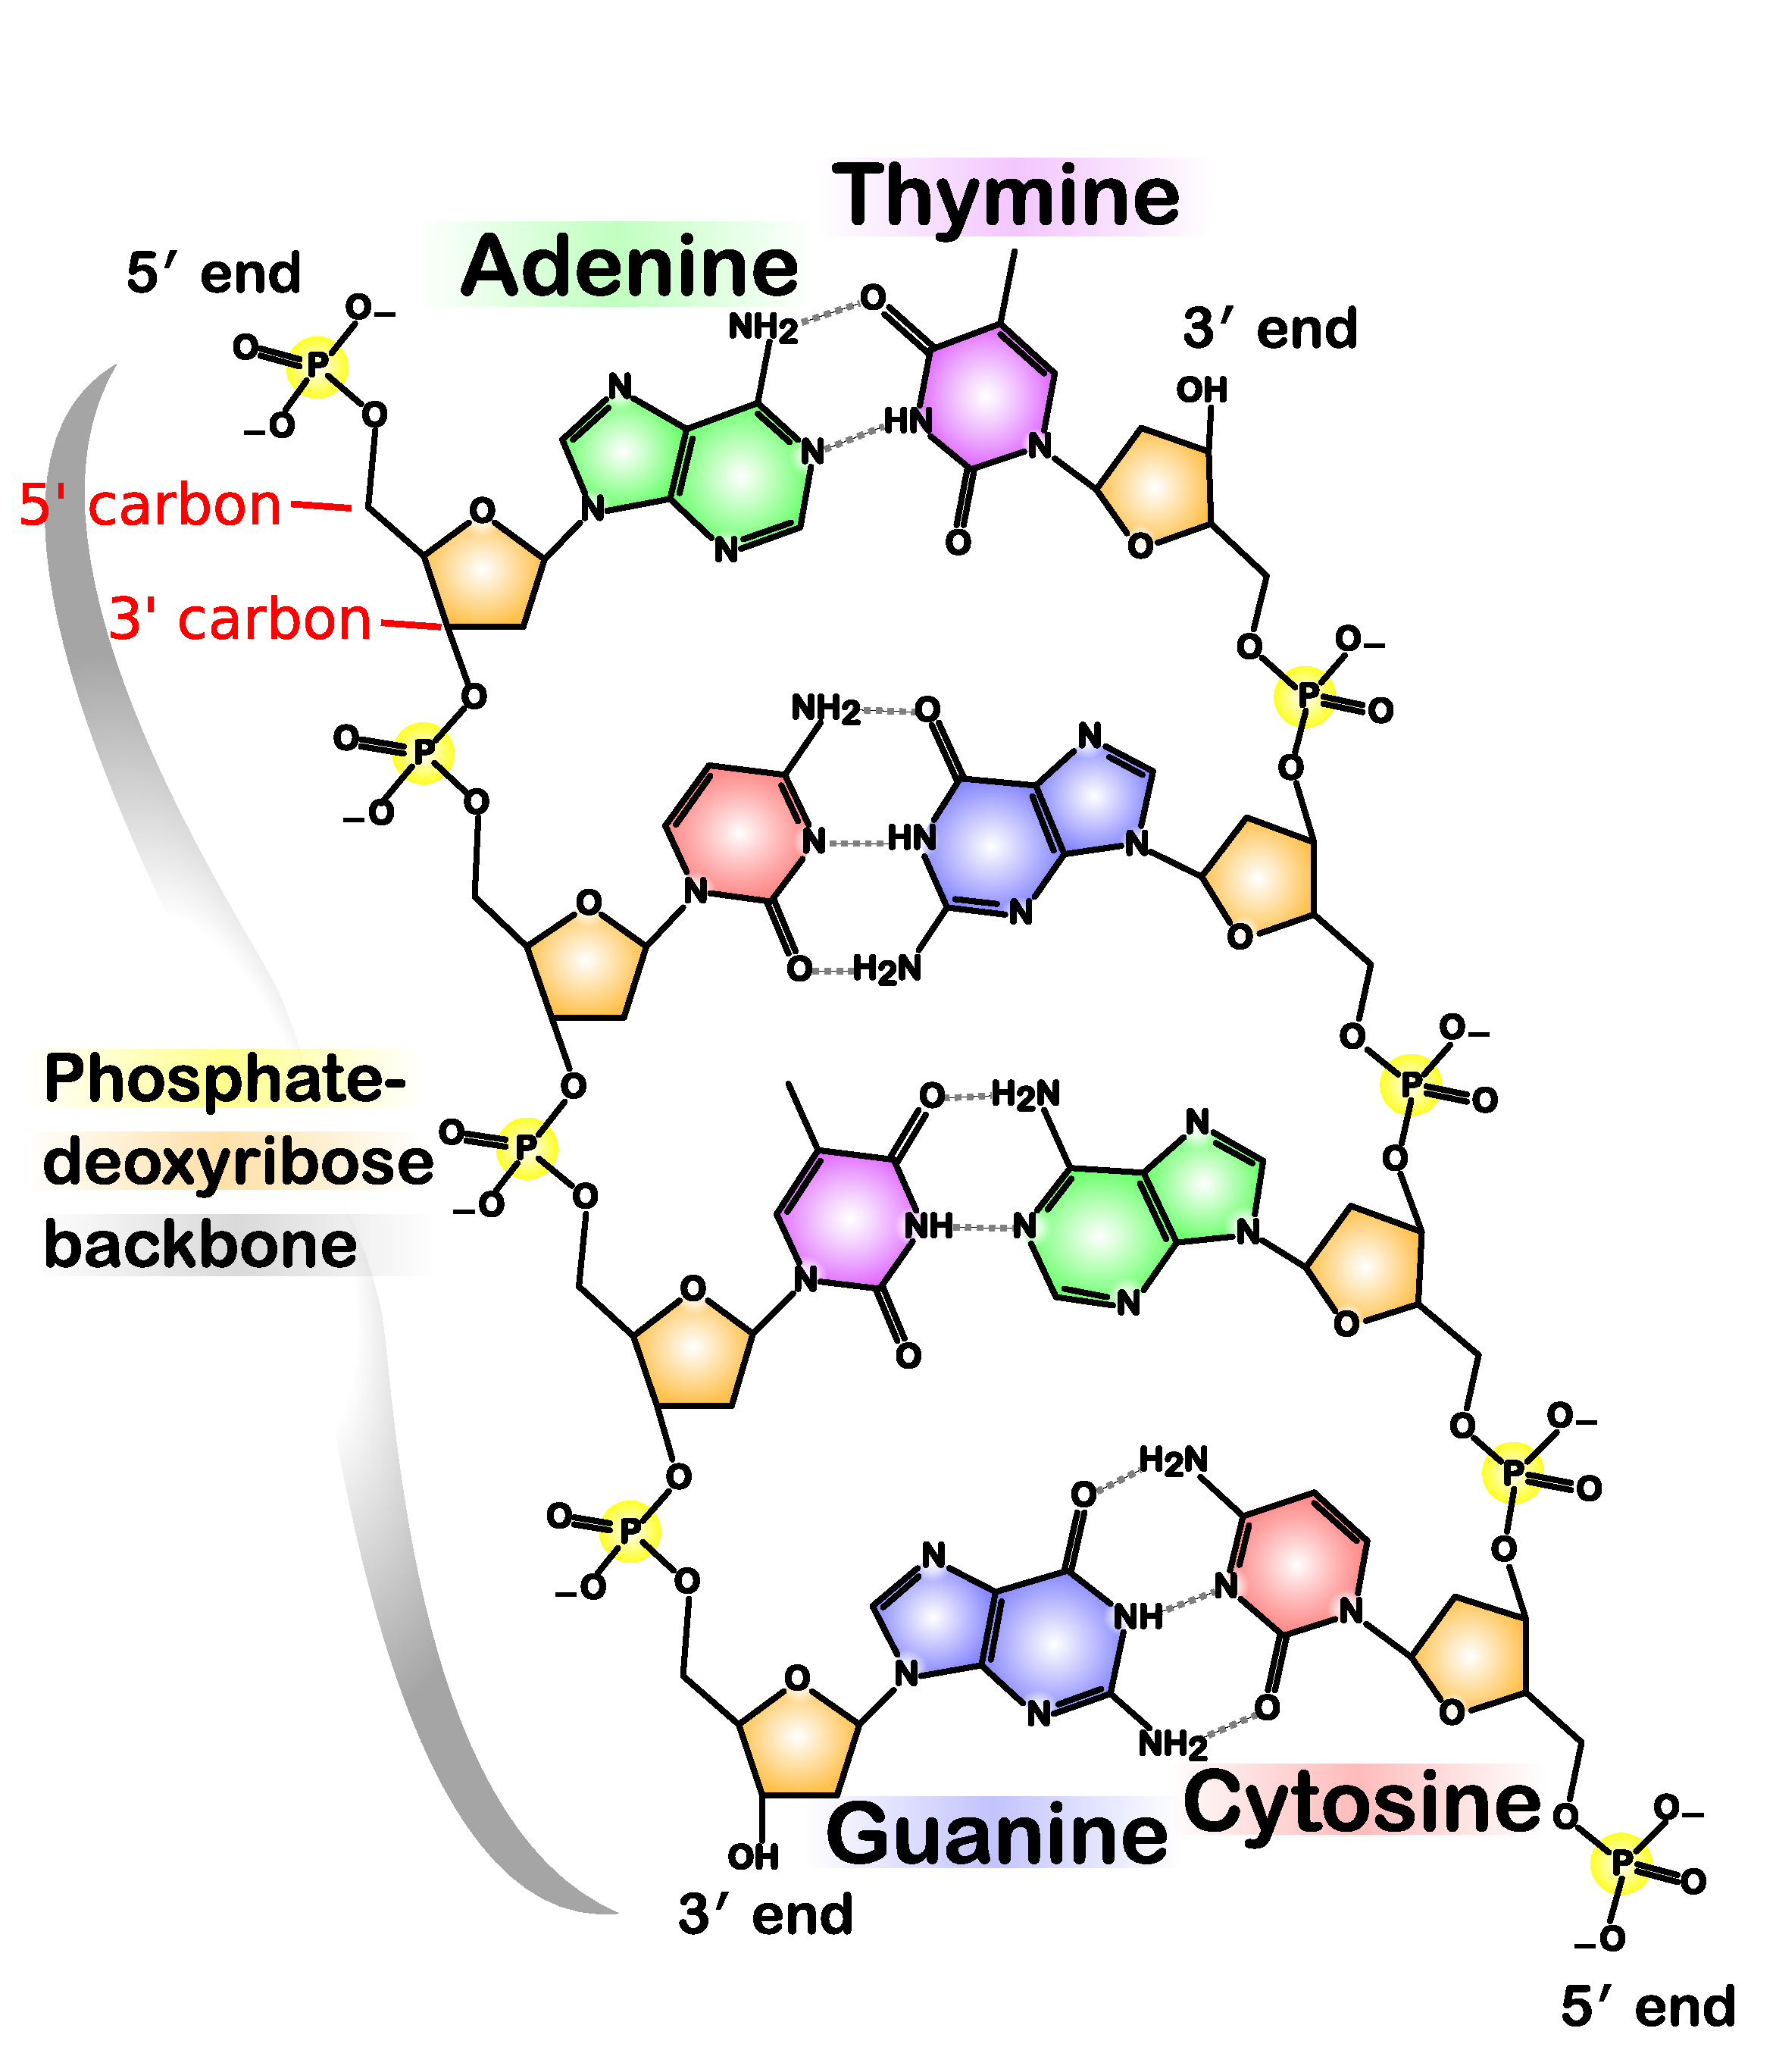
\includegraphics{figs/DNA_chemical_structure} 

}

\caption{Schematic of the structure of DNA. (Figure By Madprime (talk---contribs)  CC BY-SA 3.0, https://commons.wikimedia.org/w/index.php?curid=1848174)}\label{fig:dna-structure}
\end{figure}

The orange parts show the ribose molecules in the backbone, while the four remaining colors
denote the nucleotide bases of adenine (A), cytosine (C), guanine (G), and thymine (T). Each base
on one strand is associated with its \emph{complement} on the other strand. The hydrogen bonds between
complements is what holds the two strands of DNA together. A and T are complements, and
C and G are complements. (I remember this by noting that C and G and curvy and A and T are sharp and
angular, so the pairs go together\ldots{}).

Immediately this raises two challenges that must be resolved for making a simple,
text-based representation of DNA:

\begin{enumerate}
\def\labelenumi{\arabic{enumi}.}
\tightlist
\item
  When describing a sequence of DNA bases, which direction will we read it in?
\item
  Which strand will we read off of?
\end{enumerate}

We leave the second question until later. But note that the order in which DNA sequence
is read is, by convention, from the 5' to the 3' end of the molecule. The terms 3' and 5'
refer to different carbon atoms on the ribose backbone molecules. In the figure above,
each little ``kink'' in the ribose molecule ring (and in the attached lines) is a carbon molecule.
If you count clockwise from the oxygen in ribose, you see that the third carbon (the 3' carbon) is the
carbon atom that leads to a phosphate group, and through the phosphate, to an attachment with the
5' carbon atom of the next ribose. The 3' and 5' carbon atoms are labelled in red
on the top-left ribose molecule in Figure \ref{fig:dna-structure}.

Notice that when we speak of reading a DNA sequence, we are implicitly talking about
reading the sequence of one of the two strands of the double-stranded DNA molecule.
I'll say it again: a DNA sequence is always the sequence of one \emph{strand} of the molecule.
But, if that DNA were ``out living in the wild'' it would have been in double-stranded
form, and would have been paired with its complement sequence. For now, just note
that any DNA sequence always has a complement which is read in the reverse direction.
Thus, if we have a sequence like:

\begin{verbatim}
5'--ACTCGACCT--3'
\end{verbatim}

Then, paired with its complement it would look like:

\begin{verbatim}
5'--ACTCGACCT--3'
    |||||||||
3'--TGAGCTGGA--5'
\end{verbatim}

and, if you were to write its complement in standard 5' to 3' order,
you would have to reverse it like so:

\begin{verbatim}
5'--AGGTCGAGT--3'
\end{verbatim}

\hypertarget{dna-replication-with-dna-polymerase}{%
\subsection{DNA Replication with DNA Polymerase}\label{dna-replication-with-dna-polymerase}}

So, why do we read DNA sequence from 5' to 3'? Is it just because geneticists are wacky, backwards
folks and thought it would be fun to read in a direction that sounds, numerically, to be
backwards? No! It is because \(5'\longrightarrow 3'\) is the direction in
which a new strand of DNA is
synthesized during DNA replication.

When \citet{watsonMolecularStructureNucleic1953} published the first account of the double helical structure of DNA,
they noted that the double-helix (i.e., two-stranded) nature of the molecule immediately suggested
a copying mechanism (Figure \ref{fig:crickwat}).

\begin{figure}

{\centering 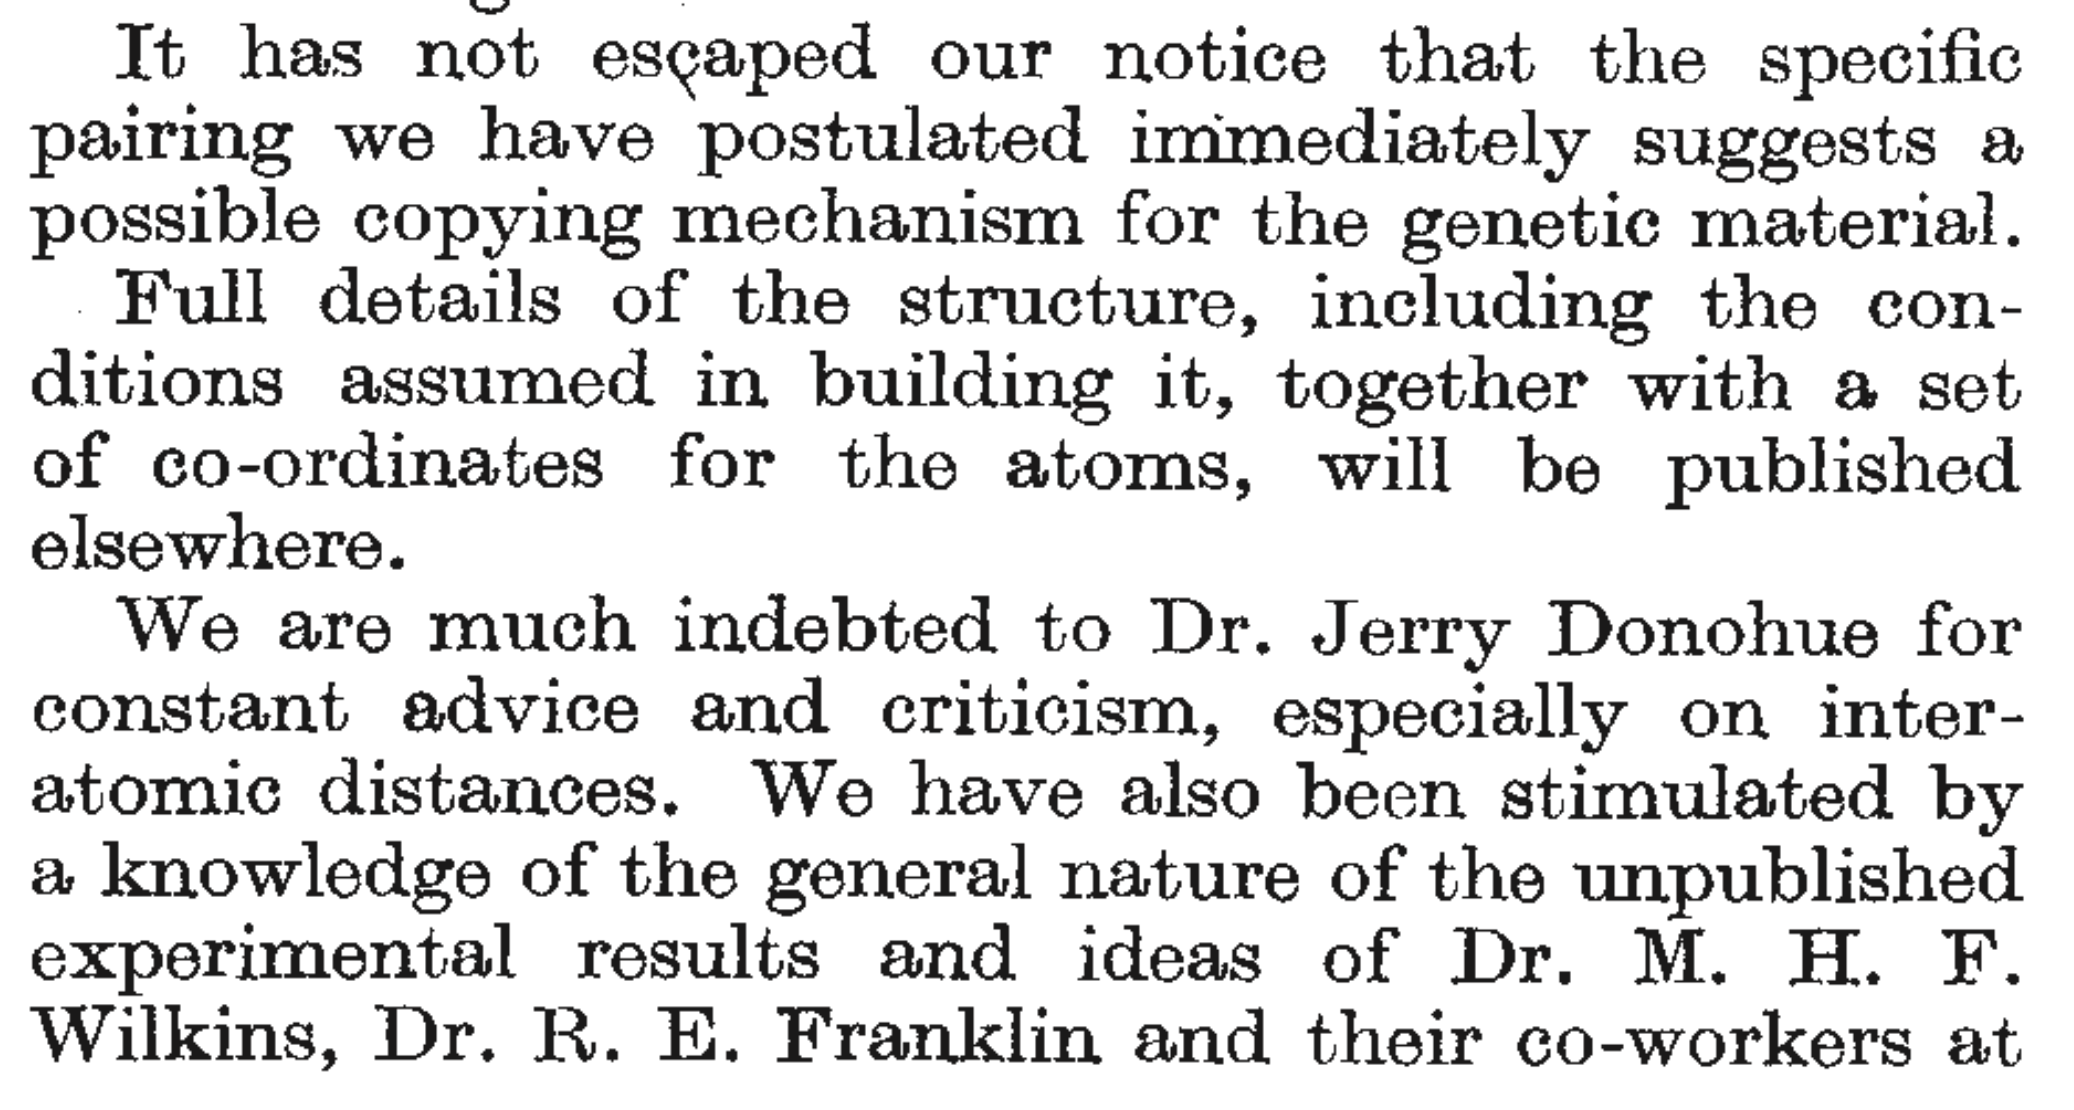
\includegraphics{figs/crick-and-watson} 

}

\caption{Excerpt from Crick and Watson (1953).}\label{fig:crickwat}
\end{figure}

(I've also included, in the excerpt, the inadequate acknowledgment
of the centrality of Rosalind Franklin's pioneering
X-ray crystallography results to Crick and Watson's conclusions---an issue in scientific history about
which much has been written, see, for example, this \href{https://www.theguardian.com/science/2015/jun/23/sexism-in-science-did-watson-and-crick-really-steal-rosalind-franklins-data}{article} in \emph{The Guardian}.)

Figure \ref{fig:dna-copying} shows a schematic of what DNA looks like during the replication process.

\begin{figure}

{\centering 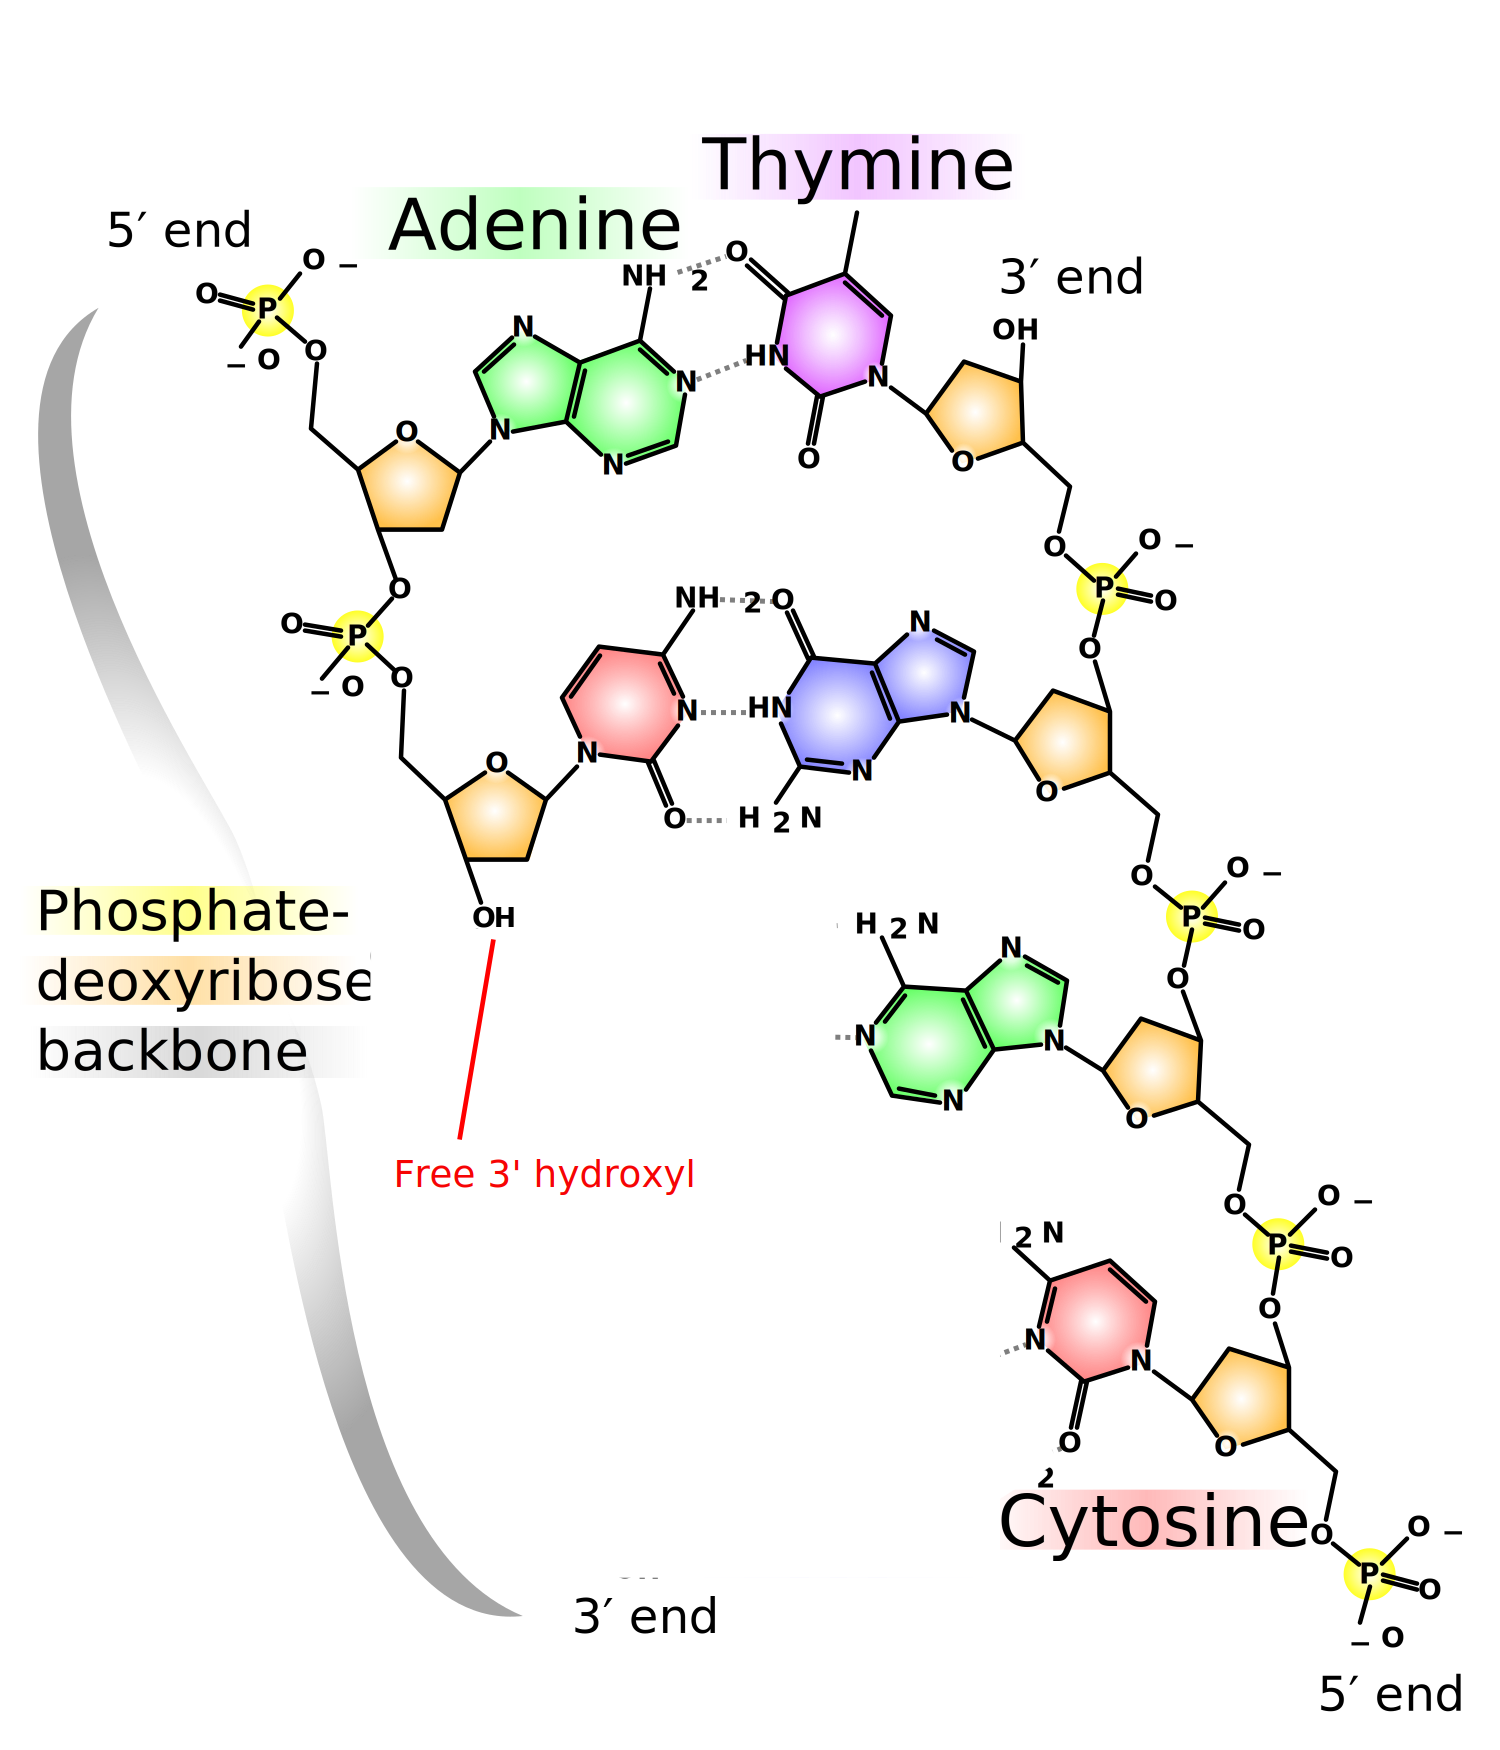
\includegraphics{figs/DNA_chemical_structure_2} 

}

\caption{DNA during replication. (Figure adapted from the one by Madprime (talk---contribs)  CC BY-SA 3.0, https://commons.wikimedia.org/w/index.php?curid=1848174)}\label{fig:dna-copying}
\end{figure}

Essentially, during DNA replication, a \emph{DNA polymerase} molecule finds nucleotide bases (attached
to three phoshpate groups) to build a new strand
that is complementary to the DNA \emph{template} strand, and it guides
those \emph{nucleotide triphosphates} to the appropriate
place in the complementary strand and helps them be incorporated into that growing,
complementary strand. The newly syntesized strand is a
\emph{reverse complement} of the template strand. However, DNA polymerase is not capable of
``setting up shop'' anywhere upon a template strand and simply stuffing complementary bases
in wherever it wants. In fact, DNA polymerase is only able to add new
bases to a growing strand if it can attach the new nucleotide triphosphate to a \emph{free 3' hydroxyl}
that is on the end of the growing strand (the 3' hydroxyl is just a hydroxyl
group attached to the 3' carbon). In Figure \ref{fig:dna-copying}, the template
strand is the strand on the right of the figure, and the growing complementary strand
is on the left side. There is a free 3' hydroxyl group on the ribose attached to the cytosine
base. That is what is needed for DNA polymerase to be able to place a
thymine triphosphate (complementary to adenine on
the template strand) in the currently vacant position. If that thymine comes with a free
3' hydroxyl group, then DNA polymerase will next place a guanine (complementary to the
cytosine on the template strand) on the growing chain. And so forth. Thus, we see
how the new strand of DNA is synthesized from the 5' to the 3' end \emph{of the growing chain}.

Of course, some people find it easier to think about a new strand of DNA being sythesized in
the 3' to 5' direction \emph{along the template strand}. This is equivalent. However, if you just remember
that ``free three'' rhymes, and that DNA polymerase needs a free 3' hydroxyl to add a new base
to the growing strand, you can always deduce that DNA must ``grow'' in a 5' to 3' direction.

\hypertarget{the-importance-of-the-3-hydroxyl}{%
\subsection{The importance of the 3' hydroxyl\ldots{}}\label{the-importance-of-the-3-hydroxyl}}

It would be hard to overstate the importance to molecular biology
of DNA polymerase's dependence upon
a free 3' hydroxyl group for new strand synthesis. This simple fact plays a central
role in:

\begin{enumerate}
\def\labelenumi{\arabic{enumi}.}
\tightlist
\item
  polymerase chain reaction (PCR)---the PCR primers are little oligonucleotides
  that attach to a template strand and provide a free 3' hydroxyl group for the initiation
  of synthesis.
\item
  a ddNTP is a nucleotide attached to a ribose molecule
  that lacks a hydroxyl group on its 3' carbon. Incorporation of
  such a ddNTP into a growing DNA strand terminates further DNA extension, and forms
  the basis for Sanger sequencing (we'll explore this below).
\item
  Some medications are designed to interfere with viral DNA replication. For example,
  AZT, or azino-thymine, is an anti-retroviral drug used to slow the progression of AIDS.
  It is a thymine nucleotide with an azino (\(\mathrm{N}_3\)) group (instead
  of a hydroxyl group) attached to the 3' carbon. Azino-thymine is used preferentially
  by reverse transcriptase when synthesizing DNA. Incorporation of it into a growing
  chain terminates DNA synthesis.
\end{enumerate}

The reversible inhibition of DNA extension also plays an important role in
sequencing by synthesis as used by Illumina platforms. We will discuss
this in a moment, but first we take a stroll down memory lane to refresh our
understanding of \emph{Sanger sequencing} so as to understand how radically different
\emph{next-generation sequencing} technologies are.

\hypertarget{sanger-sequencing}{%
\section{Sanger sequencing}\label{sanger-sequencing}}

It is hard to imagine that the first public human genome was sequenced almost
entirely by Sanger sequencing. We discuss the Sanger sequencing method
here so we can contrast it with what happens on, say, an Illumina machine
today.

To perform Sanger sequencing, first it was necessary to do PCR to
create numerous copies of a double stranded DNA fragment that was to be
sequenced. For example let's say that one wanted to sequence the
20-mer shown below, represented as double stranded DNA.

\begin{verbatim}
5'--AGGCTCAAGCTTCGACCGT--3'
3'--TCCGAGTTCGAAGCTGGCA--5'
\end{verbatim}

For Sanger sequencing, first, one would do PCR to create
bazillions of copies of that double-stranded DNA. Then four separate further PCR
reactions would be done, each one having been ``spiked'' with a little bit of
one of four different ddNTPs which, if incorporated into the
growing strand allow no further extension of it.

For example, if PCR were done as usual, but with the addition of ddATP,
then occasionally, when a ddATP (an A lacking a 3' hydroxyl group)
is incorporated into the growing strand that strand will grow no more.
Consequently, the products of that PCR (incorporating an appropriate
concentration of ddATPs), once filtered to retain only
the top strand from above, will include the fragments

\begin{verbatim}
## [1] "A*"               "AGGCTCA*"        
## [3] "AGGCTCAA*"        "AGGCTCAAGCTTCGA*"
\end{verbatim}

Where the \texttt{*} follows the sequence-terminating base.

Likewise, in a separate reaction, occasional incorporation of a ddCTP will yield products:

\begin{verbatim}
## [1] "AGGC*"              "AGGCTC*"           
## [3] "AGGCTCAAGC*"        "AGGCTCAAGCTTC*"    
## [5] "AGGCTCAAGCTTCGAC*"  "AGGCTCAAGCTTCGACC*"
\end{verbatim}

And in another reaction, occasional incorporation of ddGTP yields:

\begin{verbatim}
## [1] "AG*"                 "AGG*"               
## [3] "AGGCTCAAG*"          "AGGCTCAAGCTTCG*"    
## [5] "AGGCTCAAGCTTCGACCG*"
\end{verbatim}

And in a final, separate reaction, incorporation of ddTTP would give:

\begin{verbatim}
## [1] "AGGCT*"               "AGGCTCAAGCT*"        
## [3] "AGGCTCAAGCTT*"        "AGGCTCAAGCTTCGACCGT*"
\end{verbatim}

Each of these fragments is of a different length, so they can be
separated on an electrophoretic gel. The secret to Sanger sequencing is that
the products of all four separate reactions can be run side by side in
separate lanes of the gel (or, as was done later, in separate capillaries\ldots{}),
so that the gel, with small
fragments running faster than large fragments, from the top to the bottom
of the gel, would look like Figure \ref{fig:sanger}:
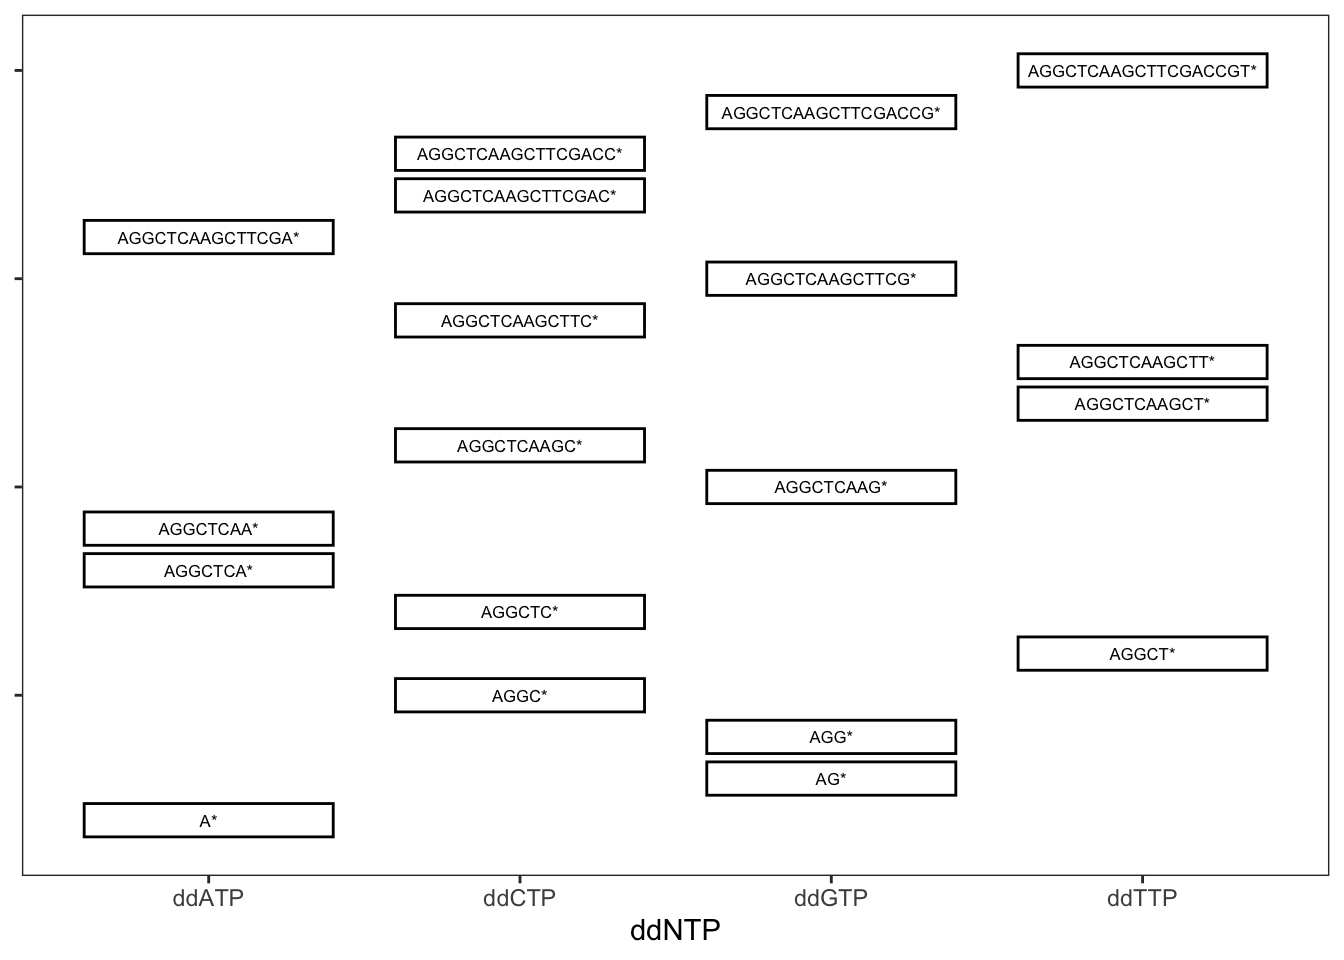
\includegraphics{eca-bioinf-handbook_files/figure-latex/sanger-1.pdf}

In reality, a gel like that in Figure \ref{fig:sanger}, won't bear the name of each
sequence fragment. In fact, it will look much more like what you see in Figure \ref{fig:sanger2}.
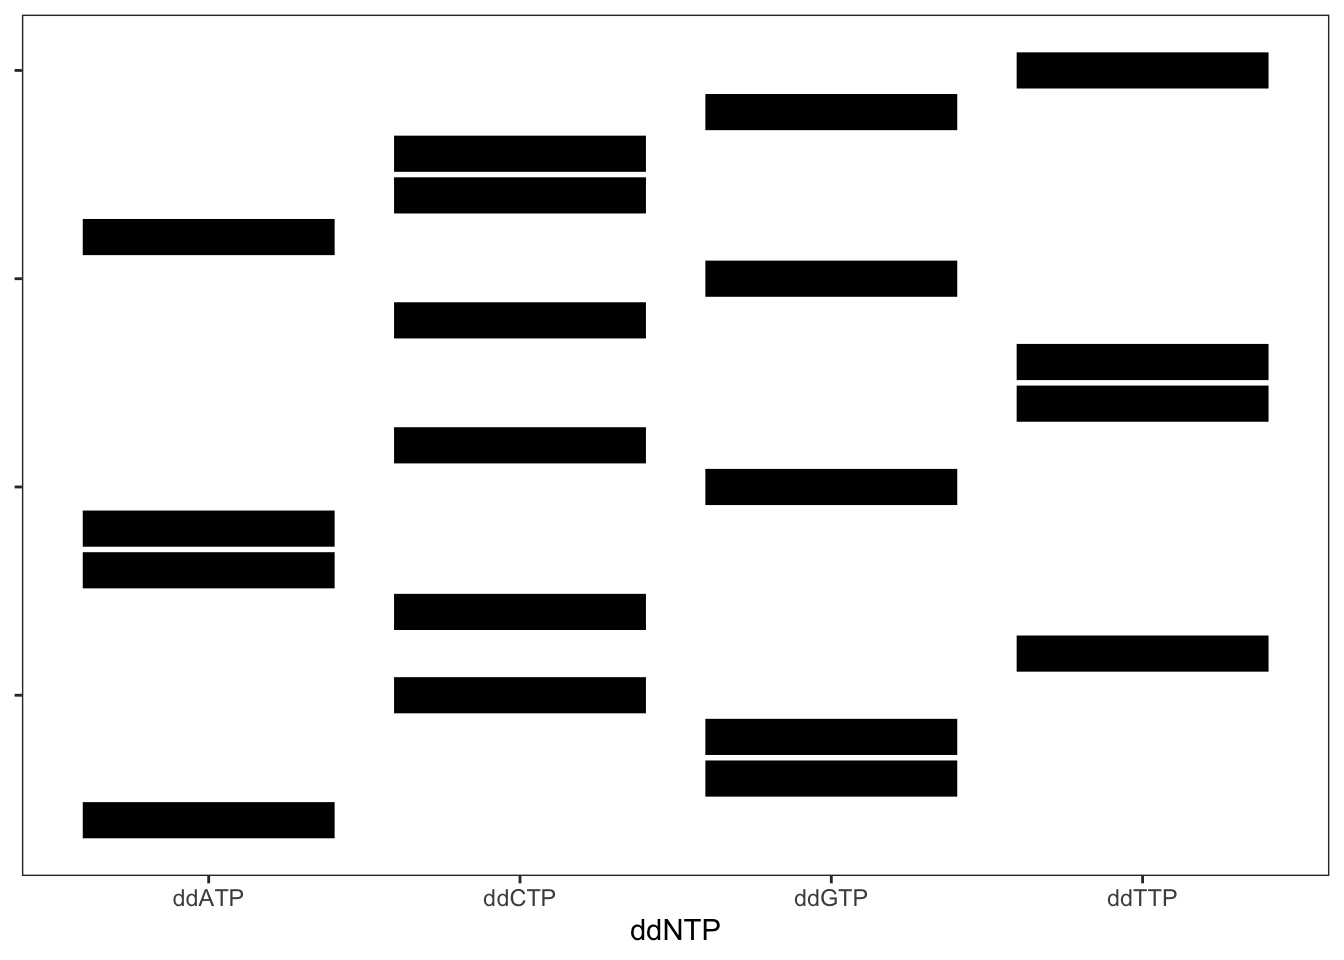
\includegraphics{eca-bioinf-handbook_files/figure-latex/sanger2-1.pdf}
However, even with the DNA fragemnt sequences obscured, their sequences can be
detemined by working from the bottom to the top and adding a different DNA base according to which column the band is in. Try it out.

Some very important points must be made about Sanger sequencing:

\begin{enumerate}
\def\labelenumi{\arabic{enumi}.}
\tightlist
\item
  The signal obtained from sequencing is, in a sense, a mixture of the starting templates. So, if you
  have DNA from an individual, you have two copies of each chromosome, and they might carry slightly
  different sequences. At heterozygous sites, it is impossible to tell which allele came from which
  chromosome.
\item
  To conduct this procedure, it was typical that specific PCR primers were used to sequence
  only a single fragment of interest. Extending the sequencing beyond that region often involved
  a laborious process of ``walking'' primers further out in either direction. Very tedious.
\item
  Each sequencing reaction was typically carried out for just a single individual at once.\\
\item
  Until a little over a decade ago, this is how sequencing was done in conservation genetics.
\end{enumerate}

\hypertarget{illumina-sequencing-by-synthesis}{%
\section{Illumina Sequencing by Synthesis}\label{illumina-sequencing-by-synthesis}}

Illumina paired-end sequencing is currently the leading technology in conservation
genomics.

They say that a picture is worth a thousand words, so a video may well be worth
ten thousand. Illumina has a very informative video about sequencing by synthesis.

I have used some code (I found on GitHub) to provide captions to the video. These captions
include comments, as well as questions that form part of this week's homework. (Yay!)\\
You can see the video at
\url{https://eriqande.github.io/erics-captioned-vids/vids/illumina-sbs/}

The main take-home messages I want everyone to get about Illumin sequencing is:

\begin{enumerate}
\def\labelenumi{\arabic{enumi}.}
\tightlist
\item
  The signal obtained from each cluster is the sequence of a single, \emph{single-stranded DNA fragment}
\item
  In paired-end sequencing, sequence from both ends of the fragment (but not necessarily
  the middle) is obtained.
\item
  The technique lends itself to sequencing millions of ``anonymous'' chunks of DNA.
\item
  The indexes, or ``barcodes'' allow DNA from multiple individuals to be sequenced in a single run.
\item
  This is how most high-throughput sequencing is done today.
\end{enumerate}

\hypertarget{library-prep-protocols}{%
\section{Library Prep Protocols}\label{library-prep-protocols}}

Gotta mention here about how barcodes work.

How you prepare your libraries dictates what type of data you get.

\hypertarget{wgs}{%
\subsection{WGS}\label{wgs}}

\hypertarget{rad-seq-methods}{%
\subsection{RAD-Seq methods}\label{rad-seq-methods}}

\hypertarget{amplicon-sequencing}{%
\subsection{Amplicon Sequencing}\label{amplicon-sequencing}}

\hypertarget{capture-arrays-rapture-etc.}{%
\subsection{Capture arrays, RAPTURE, etc.}\label{capture-arrays-rapture-etc.}}

\hypertarget{bioinformatic-file-formats-and-associated-tools}{%
\chapter{Bioinformatic file formats and associated tools}\label{bioinformatic-file-formats-and-associated-tools}}

Almost all the high-throughput sequencing data you will deal with should
arrive in just a few different formats. There are some specialized formats
(like those output by the program TASSEL, etc.) but we will largely ignore
those, focusing instead on the format used in production by the 1000 genomes
and 10K vertebrate genomes projects. In a sentence, the most important are:
FASTA, FASTQ, SAM, BAM, and VCF.

Plan: Go over these, and for each, pay special attention to compressed and indexed
forms and explain why that is so important. I think that we should probably
talk about the programs that are available for manipulating each of these, as well,
but I won't add that until we all have access to an HPC or other proper
Unix environment.

\hypertarget{sequences}{%
\section{Sequences}\label{sequences}}

\hypertarget{fasta}{%
\section{FASTA}\label{fasta}}

Come back to this when we talk about alignments.

\hypertarget{fastq}{%
\section{FASTQ}\label{fastq}}

The FASTQ format is the standard format for lightly-processed data
coming off an Illumina machine. If you are doing whole genome sequencing,
it is typical for the Illumina processing pipeline to have separated all
the reads with different barcodes into different, separate files. Typically
this means that all the reads from one library prep for one sample will
be in a single file. The barcodes and any associated additional adapter
sequence is typically also removed from the reads. If you are processing
RAD data, the reads may not be separated by barcode, because, due to the
vagaries of the RAD library prep, the barcodes might appear on different ends
of some reads than expected.

A typical file extension for FASTQ files is \texttt{.fq}.
Almost all FASTQ files you get from a sequencer should be gzipped to save space.
Thus, in order to view the file you will have to uncompress it. Since you would,
in most circumstances, want to visually inspect just a few lines, it is best
to do that with \texttt{gzcat} and pipe the output to \texttt{head}.

As we have seen, paired-end sequencing produces two separate reads of a DNA
fragment. Those two different reads are usually stored in two separate files named
in such a manner as to transparently denote whether it contains sequences obtained
from read 1 or read 2.
For example \texttt{bird\_08\_B03\_R1.fq.gz} and \texttt{bird\_08\_B03\_R2.fq.gz}. Read 1 and Read 2 from
a paired read must occupy the sames lines in their respective files, i.e., lines
10001-10004 in \texttt{bird\_08\_B03\_R1.fq.gz} and lines 10001-10004 in \texttt{bird\_08\_B03\_R2.fq.gz}
should both pertain to the same DNA fragment that was sequenced. That is what is
meant by ``paired-end'' sequencing: the sequences come in pairs from different
ends of the same fragment.

The FASTQ format is \emph{very} simple: information about each read occupies just four lines.
This means that the number of lines in a proper FASTQ file must always be a multiple of four.
Briefly, the four lines of information about each read are always in the same order as follows:

\begin{enumerate}
\def\labelenumi{\arabic{enumi}.}
\tightlist
\item
  An Identifier line
\item
  The DNA sequence as A's, C's, G's and T's.
\item
  A line that is almost always simply a \texttt{+} sign, but can optionally be followed
  by a repeat of the ID line.
\item
  An ASCII-encoded, Phred-scaled base quality score. This gives an estimated
  measure of certainty about each base call in the sequence.
\end{enumerate}

The code block below shows three reads worth (twelve lines) of
information from a FASTQ file.
Take a moment to identify the four different lines for each read.

\begin{verbatim}
@K00364:64:HTYYCBBXX:1:1108:4635:14133/1
TAGAATACGCCAGGTGTAAGAATAGTAGAATACGCCAGGTGTAAGAATAGTAGAACACGCCAGGTGTAAGAATAGTAGAA
+
AAAFFJJJJJFFJFJJJFJJFFJFJFJJJJJJJJFFJJJFJJJFJJAJJFJJFJJFJJJ7JJJF-<JAFJJ<F<AJAJJF
@K00364:64:HTYYCBBXX:1:1108:5081:25527/1
AAAACACCAAAAGAAAGATGCCCAGGGTCCCTGCTCATCTGCGTGAAAGTGACTTAGGCATGCTGCAAGGAGGCATGAGG
+
AAFFFJJJJJJJJJJJJJJJJJJJJJJJJJJJJJJJJJJJJJJJJJJJJJJJJJJJJJJJJJJJJJJJJJJJJJJJJJJJ
@K00364:64:HTYYCBBXX:1:1108:5852:47295/1
AGGTGGCTCTAGAAGGTTCTCGGACCGAGAAACAGCCTCGTACATTTGCAATGATTTCAATTCATTTTGACCATTACGAA
+
AAFFFJJJJJJJJJJJJJJJJJJJJJJJJJJJJJJJJJJJJJJJJJJJJJJJJJJJJJJJJJJJJJJJJJJJJJJJJJJJ
\end{verbatim}

Lines 2 and 3 are self-explanatory, but we will expound upon lines 1 and 4 below.

\hypertarget{line-1-illumina-identifier-lines}{%
\subsection{Line 1: Illumina identifier lines}\label{line-1-illumina-identifier-lines}}

The identifier line can be just about any string that starts with an \texttt{@}, but, from Illumina data, today,
you will typically see something like this:

\begin{verbatim}
@K00364:64:HTYYCBBXX:1:1108:4635:14133/1
\end{verbatim}

The colons (and the \texttt{/}) are field separators. The separate parts of the line
above are interpreted something along the lines as follows (keeping in mind that
Illumina occasionally changes the format and that there may be additional
optional fields):

\begin{verbatim}
@           : mandatory character that starts the ID line
K00364      : Unique sequencing machine ID 
64          : Run number on instrument
HTYYCBBXX   : Unique flow cell identifier
1           : Lane number
1108        : Tile number (section of the lane)
4635        : x-coordinate of the cluster within the tile
14133       : y-coordinate of the cluster within the tile
1           : Whether the sequence is from read 1 or read 2 
\end{verbatim}

Question: For paired reads, do you expect the x- and y-coordinates for read 1 and read 2 to
be the same?

\hypertarget{line-4-base-quality-scores}{%
\subsection{Line 4: Base quality scores}\label{line-4-base-quality-scores}}

The base quality scores give an estimate of the probability that the base call is incorrect.
This comes from data the sequencer collects on the brightness and compactness of the cluster
radiance, other factors, and Illumina's own models for base call accuracy. If we let \(p\)
be the probability that a base is called incorrectly, then \(Q\), the Phred-scaled base quality
score, is:

\[
Q = \lfloor-10\log_{10}p\rfloor,
\]
where \(\lfloor x \rfloor\) means "the largest integer smaller than \(x\).

To get the estimate of the probability that the base is called incorrectly from
the Phred scaled score, you invert the above equation:

\[
p = \frac{1}{10^{Q/10}}
\]
Base quality scores from Illumina range from 0 to 40.
The easiest values to use as guideposts are \(Q = 0, 10, 20, 30, 40\), which correspond to
error probabilites of 1, 1 in 10, 1 in 100, 1 in 1,000, and 1 in 10,000, respectively.

All this is fine and well, but when we look at the quality score line above we see
something like \texttt{7JJJF-\textless{}JAFJJ\textless{}F\textless{}AJAJJF}. What gives? Well, from a file storage and
parsing perspective, it makes sense to only use a single character to store the
quality score for every base. So, that is what has been done: each of those
single characters represents a quality score---a number between 0 and 40, inclusive.

The values that have been used are the \emph{decimal representations of ASCII text characters} minus 33.\\
The decimal representation or each character can be found in Figure \ref{fig:ascii}.

\begin{figure}

{\centering 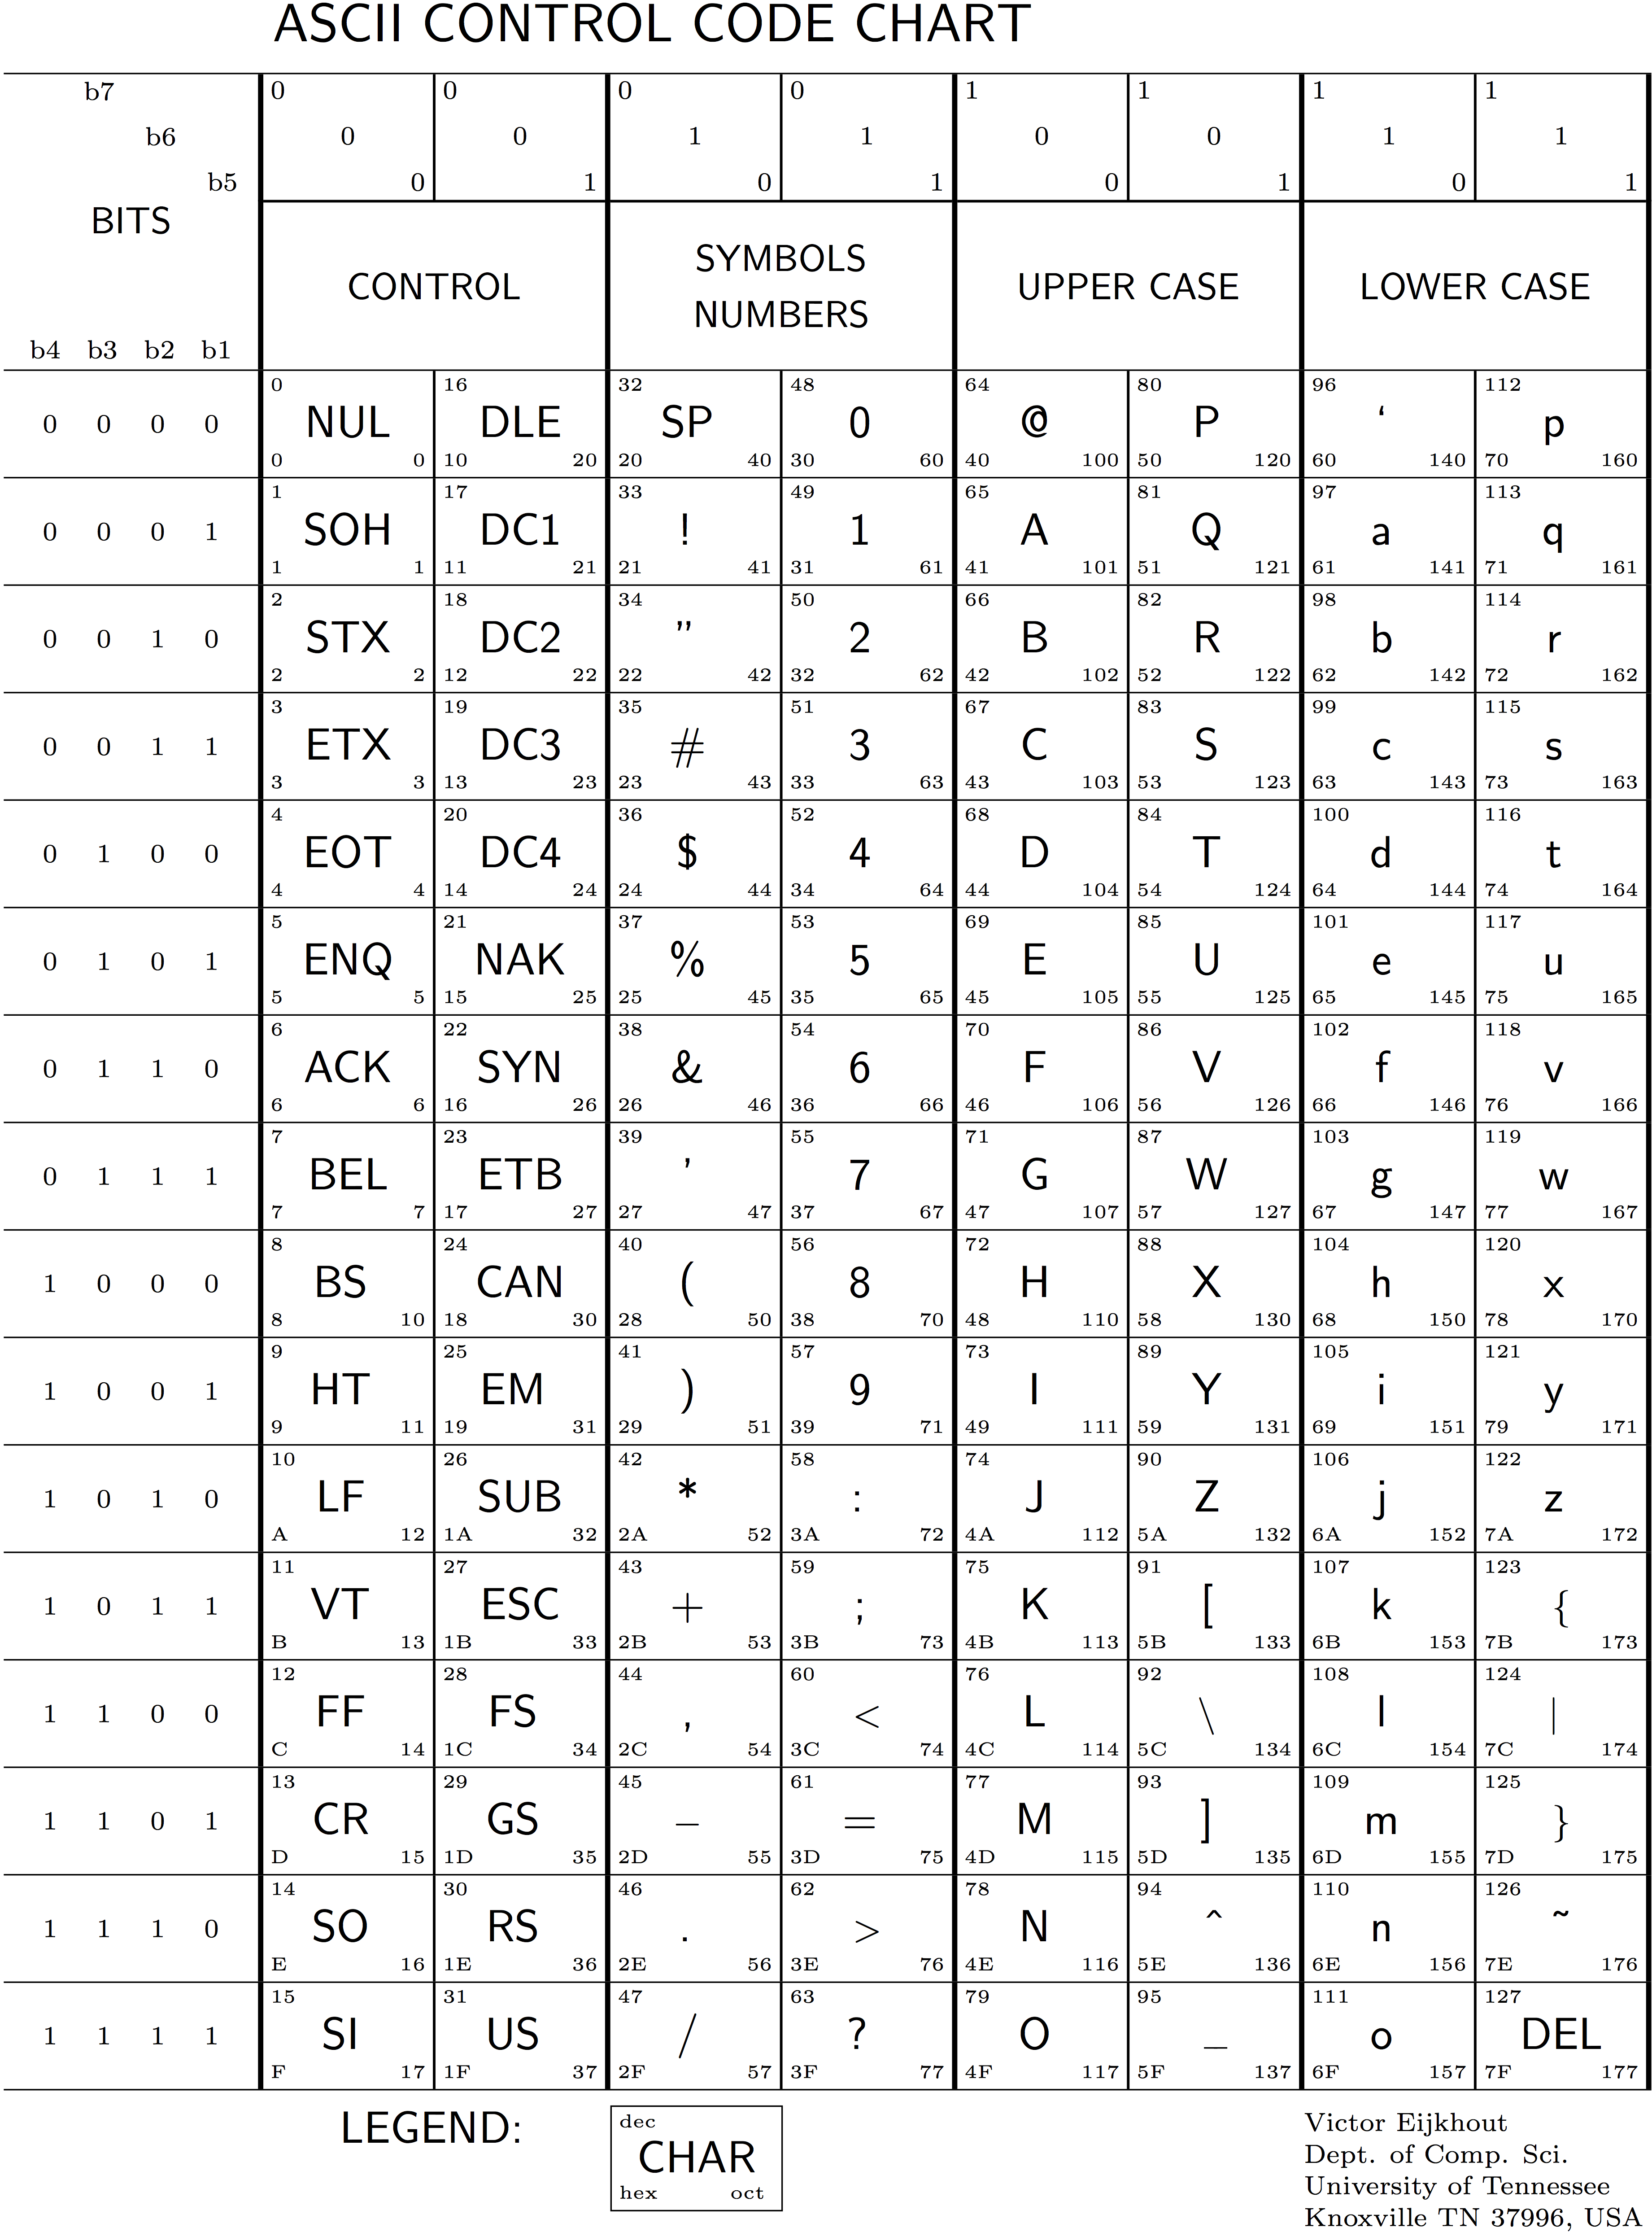
\includegraphics{figs/ascii-crop} 

}

\caption{This lovely ASCII table shows the binary, hexadecimal, octal and decimal representations of ASCII characters (in the corners of each square; see the legend rectangle at bottom.  Table produced from TeX code written and developed by Victor Eijkhout available at [https://ctan.math.illinois.edu/info/ascii-chart/ascii.tex](https://ctan.math.illinois.edu/info/ascii-chart/ascii.tex)}\label{fig:ascii}
\end{figure}

The decimal representation in in the upper left of each character's rectangle.

Find the characters corresponding to base quality scores of 0, 10, 20, 30, and 40. Remember that the
base quality score is the character's decimal representation \emph{minus 33}.

Here is another question: why do you think the scale starts with ASCII character 33?

\hypertarget{a-fastq-tidyverse-interlude}{%
\subsection{A FASTQ `tidyverse' Interlude}\label{a-fastq-tidyverse-interlude}}

Here we demonstrate some R code while exploring FASTQ files. First, in order to
do these exercises you will want to download and launch the RStudio project,
\texttt{big-fastq-play},
that has the data
in it. Please work within that RStudio project to do these exercises.
Here is a direct download link to it:
\url{https://docs.google.com/uc?export=download\&id=1iD8tz_KSOHDBpXvXssqo3noPZAm1Qsjp}

Note that this might stress out older laptops as it loads 100s of Mb of sequence
data into memory.

\hypertarget{reading-fastqs-with-read_lines}{%
\subsubsection{\texorpdfstring{Reading FASTQs with \texttt{read\_lines}}{Reading FASTQs with read\_lines}}\label{reading-fastqs-with-read_lines}}

Load packages:

\begin{Shaded}
\begin{Highlighting}[]
\KeywordTok{library}\NormalTok{(tidyverse)}

\CommentTok{# if you don't have this package, get it}
\CommentTok{# install.packages("viridis")}
\KeywordTok{library}\NormalTok{(viridis)}
\end{Highlighting}
\end{Shaded}

Read the FASTQ, make it a matrix, then make it a tibble

\begin{Shaded}
\begin{Highlighting}[]
\CommentTok{# use read_lines to read the R1 fastq file line by line;}
\CommentTok{# then make a 4 column matrix, filling by rows}
\CommentTok{# then drop column 3, which corresponds to the "+" line}
\NormalTok{R1 <-}\StringTok{ }\KeywordTok{read_lines}\NormalTok{(}\StringTok{"data/Battle_Creek_01_chinook_R1.fq.gz"}\NormalTok{) }\OperatorTok
\StringTok{  }\KeywordTok{matrix}\NormalTok{(}\DataTypeTok{ncol =} \DecValTok{4}\NormalTok{, }\DataTypeTok{byrow =} \OtherTok{TRUE}\NormalTok{) }\OperatorTok
\StringTok{  }\NormalTok{.[,}\OperatorTok{-}\DecValTok{3}\NormalTok{]}
  

\CommentTok{# add colnames}
\KeywordTok{colnames}\NormalTok{(R1) <-}\StringTok{ }\KeywordTok{c}\NormalTok{(}\StringTok{"ID"}\NormalTok{, }\StringTok{"seq"}\NormalTok{, }\StringTok{"qual"}\NormalTok{)}

\CommentTok{# now make a tibble out that.  We will assign}
\CommentTok{# it back to the variable R1, to note carry}
\CommentTok{# extra memory around}
\NormalTok{R1 <-}\StringTok{ }\KeywordTok{as_tibble}\NormalTok{(R1)}

\CommentTok{# Look at it:}
\NormalTok{R1}


\CommentTok{# OK, 1 million reads.}
\end{Highlighting}
\end{Shaded}

Look at the first ID line:

\begin{verbatim}
 @E00430:101:HKT7WCCXY:1:1101:6411:1204 1:N:0:NGATGT
\end{verbatim}

Aha! This is a slightly different format than the above. The part after the
space has colon-separated fields that are:

\begin{verbatim}
1        :  which read of the pair
N        :  has this been filtered (Y/N)
0        :  control number (always 0 on HiSeq and NextSeq)
NGATGT   :  barcode on the read
\end{verbatim}

OK, our mission is to actually look at the locations of these reads on different
tiles. To do that we will want to access the x and y coordinates and the
tiles, etc. In the tidyverse, this means giving each of those things its own
column.

\hypertarget{tidyrseparate}{%
\subsubsection{tidyr::separate()}\label{tidyrseparate}}

How do we break those colon-separated fields into columns? This is a job for
\texttt{tidyr::separate} which breaks a text string on user-defined separators into
columns in a tibble.

Here we can use it to break the ID into two parts split on the space, and then
break the first part of the ID into its constituent parts:

\begin{Shaded}
\begin{Highlighting}[]
\CommentTok{# first we break on the space,}
\CommentTok{# then we break the ID on the colons, but keep the original "id" for later}
\NormalTok{R1 }\OperatorTok
\StringTok{  }\KeywordTok{separate}\NormalTok{(ID, }\DataTypeTok{into =} \KeywordTok{c}\NormalTok{(}\StringTok{"id"}\NormalTok{, }\StringTok{"part2"}\NormalTok{), }\DataTypeTok{sep =} \StringTok{" "}\NormalTok{) }\OperatorTok
\StringTok{  }\KeywordTok{separate}\NormalTok{(}
\NormalTok{    id, }
    \DataTypeTok{into =} \KeywordTok{c}\NormalTok{(}\StringTok{"machine"}\NormalTok{, }\StringTok{"run"}\NormalTok{, }\StringTok{"flow_cell"}\NormalTok{, }\StringTok{"lane"}\NormalTok{, }\StringTok{"tile"}\NormalTok{, }\StringTok{"x"}\NormalTok{, }\StringTok{"y"}\NormalTok{), }
    \DataTypeTok{sep =} \StringTok{":"}\NormalTok{,}
    \DataTypeTok{remove =} \OtherTok{FALSE}
\NormalTok{    )}
\end{Highlighting}
\end{Shaded}

Wow! That was cool. Now, your mission is to pipe that (with \texttt{\%\textgreater{}\%})
into another \texttt{separate()} command that breaks part2 into
\texttt{read}, \texttt{filter}, \texttt{cnum}, and \texttt{barcode}, and save that into \texttt{R1\_sep}

Here is a starter:

\begin{Shaded}
\begin{Highlighting}[]
\NormalTok{R1_sep <-}\StringTok{ }\NormalTok{R1 }\OperatorTok
\StringTok{  }\KeywordTok{separate}\NormalTok{(ID, }\DataTypeTok{into =} \KeywordTok{c}\NormalTok{(}\StringTok{"id"}\NormalTok{, }\StringTok{"part2"}\NormalTok{), }\DataTypeTok{sep =} \StringTok{" "}\NormalTok{) }\OperatorTok
\StringTok{  }\KeywordTok{separate}\NormalTok{(}
\NormalTok{    id, }
    \DataTypeTok{into =} \KeywordTok{c}\NormalTok{(}\StringTok{"machine"}\NormalTok{, }\StringTok{"run"}\NormalTok{, }\StringTok{"flow_cell"}\NormalTok{, }\StringTok{"lane"}\NormalTok{, }\StringTok{"tile"}\NormalTok{, }\StringTok{"x"}\NormalTok{, }\StringTok{"y"}\NormalTok{), }
    \DataTypeTok{sep =} \StringTok{":"}\NormalTok{,}
    \DataTypeTok{remove =} \OtherTok{FALSE}
\NormalTok{    ) }\OperatorTok
\StringTok{    }\NormalTok{...your code here...}
    
\CommentTok{# when you are done with that, look at it}
\NormalTok{R1_sep}
    
\end{Highlighting}
\end{Shaded}

Doh! There is one thing to note. Look at the first few columns of that:

\begin{Shaded}
\begin{Highlighting}[]
\CommentTok{# A tibble: 1,000,000 x 11}
\NormalTok{   id          machine run   flow_cell lane  tile  x     y   }
   \OperatorTok{<}\NormalTok{chr}\OperatorTok{>}\StringTok{       }\ErrorTok{<}\NormalTok{chr}\OperatorTok{>}\StringTok{   }\ErrorTok{<}\NormalTok{chr}\OperatorTok{>}\StringTok{ }\ErrorTok{<}\NormalTok{chr}\OperatorTok{>}\StringTok{     }\ErrorTok{<}\NormalTok{chr}\OperatorTok{>}\StringTok{ }\ErrorTok{<}\NormalTok{chr}\OperatorTok{>}\StringTok{ }\ErrorTok{<}\NormalTok{chr}\OperatorTok{>}\StringTok{ }\ErrorTok{<}\NormalTok{chr}\OperatorTok{>}\StringTok{      }
\StringTok{ }\DecValTok{1} \OperatorTok{@}\NormalTok{E00430}\OperatorTok{:}\NormalTok{10… }\OperatorTok{@}\NormalTok{E00430 }\DecValTok{101}\NormalTok{   HKT7WCCXY }\DecValTok{1}     \DecValTok{1101}  \DecValTok{6411}  \DecValTok{1204}
 \DecValTok{2} \OperatorTok{@}\NormalTok{E00430}\OperatorTok{:}\NormalTok{10… }\OperatorTok{@}\NormalTok{E00430 }\DecValTok{101}\NormalTok{   HKT7WCCXY }\DecValTok{1}     \DecValTok{1101}  \DecValTok{7324}  \DecValTok{1204}
 \DecValTok{3} \OperatorTok{@}\NormalTok{E00430}\OperatorTok{:}\NormalTok{10… }\OperatorTok{@}\NormalTok{E00430 }\DecValTok{101}\NormalTok{   HKT7WCCXY }\DecValTok{1}     \DecValTok{1101}  \DecValTok{8582}  \DecValTok{1204}
 \DecValTok{4} \OperatorTok{@}\NormalTok{E00430}\OperatorTok{:}\NormalTok{10… }\OperatorTok{@}\NormalTok{E00430 }\DecValTok{101}\NormalTok{   HKT7WCCXY }\DecValTok{1}     \DecValTok{1101}  \DecValTok{9841}  \DecValTok{1204}
 \DecValTok{5} \OperatorTok{@}\NormalTok{E00430}\OperatorTok{:}\NormalTok{10… }\OperatorTok{@}\NormalTok{E00430 }\DecValTok{101}\NormalTok{   HKT7WCCXY }\DecValTok{1}     \DecValTok{1101}  \DecValTok{10186} \DecValTok{1204} 
\end{Highlighting}
\end{Shaded}

The x- and the y-coordinates are listed as characters (\texttt{\textless{}chr\textgreater{}}) but they should
be numeric. This shows the default behavior of \texttt{separate()}: it just breaks each
field into a column of strings. However, you can ask \texttt{separate()} to make a good-faith
guess of the type of each column and convert it to that. This works suitably in this
situation, so, let's repeat the last command, but convert types automatically:

\begin{Shaded}
\begin{Highlighting}[]
\NormalTok{R1_sep <-}\StringTok{ }\NormalTok{R1 }\OperatorTok
\StringTok{  }\KeywordTok{separate}\NormalTok{(ID, }\DataTypeTok{into =} \KeywordTok{c}\NormalTok{(}\StringTok{"id"}\NormalTok{, }\StringTok{"part2"}\NormalTok{), }\DataTypeTok{sep =} \StringTok{" "}\NormalTok{) }\OperatorTok
\StringTok{  }\KeywordTok{separate}\NormalTok{(}
\NormalTok{    id, }
    \DataTypeTok{into =} \KeywordTok{c}\NormalTok{(}\StringTok{"machine"}\NormalTok{, }\StringTok{"run"}\NormalTok{, }\StringTok{"flow_cell"}\NormalTok{, }\StringTok{"lane"}\NormalTok{, }\StringTok{"tile"}\NormalTok{, }\StringTok{"x"}\NormalTok{, }\StringTok{"y"}\NormalTok{), }
    \DataTypeTok{sep =} \StringTok{":"}\NormalTok{,}
    \DataTypeTok{remove =} \OtherTok{FALSE}\NormalTok{,}
    \DataTypeTok{convert =} \OtherTok{TRUE}
\NormalTok{  ) }\OperatorTok
\StringTok{  }\KeywordTok{separate}\NormalTok{(part2, }\DataTypeTok{into =} \KeywordTok{c}\NormalTok{(}\StringTok{"read"}\NormalTok{, }\StringTok{"filter"}\NormalTok{, }\StringTok{"cnum"}\NormalTok{, }\StringTok{"barcode"}\NormalTok{), }\DataTypeTok{sep =} \StringTok{":"}\NormalTok{, }\DataTypeTok{convert =} \OtherTok{TRUE}\NormalTok{)}
\end{Highlighting}
\end{Shaded}

\hypertarget{counting-tiles}{%
\subsubsection{Counting tiles}\label{counting-tiles}}

Let's see how many tiles these reads came from. Basically we just want to count the
number of rows with different values for tile. Read the documentation for
\texttt{dplyr::count} with

\begin{Shaded}
\begin{Highlighting}[]
\NormalTok{?count}
\end{Highlighting}
\end{Shaded}

and when you are done count up the number of reads in each tile:

\begin{Shaded}
\begin{Highlighting}[]
\NormalTok{R1_sep }\OperatorTok
\StringTok{  }\NormalTok{...your code here...}
\end{Highlighting}
\end{Shaded}

Turns out they are all from the same tile\ldots{}

\hypertarget{parsing-quality-scores}{%
\subsubsection{Parsing quality scores}\label{parsing-quality-scores}}

Now, we want to turn the quality-score ASCII-characters into Phred-scaled
qualities, ultimately taking the average over each sequence of those.

Check out this function:

\begin{Shaded}
\begin{Highlighting}[]
\KeywordTok{utf8ToInt}\NormalTok{(}\StringTok{"!*JGH"}\NormalTok{)}
\end{Highlighting}
\end{Shaded}

\begin{verbatim}
## [1] 33 42 74 71 72
\end{verbatim}

We can use that to get Phred-scaled values by subtracting 33 from the result. Let's check:

\begin{Shaded}
\begin{Highlighting}[]
\KeywordTok{utf8ToInt}\NormalTok{(}\StringTok{"!+5?IJ"}\NormalTok{) }\OperatorTok{-}\StringTok{ }\DecValTok{33}
\end{Highlighting}
\end{Shaded}

\begin{verbatim}
## [1]  0 10 20 30 40 41
\end{verbatim}

Note that \texttt{J} seems to be used for ``below 1 in 10,000'' as it is the highest I have ever seen.

So, what we want to do is make a new column called \texttt{mean\_qual} that gives the
mean of the Phred-scaled qualities. Any time you need to make a new column in a
tibble, where the result in each row depends only on the values in current columns
in that same row, that is a job for \texttt{mutate()}.

However, in this case, because the \texttt{utf8ToInt()} function doesn't take vector input,
computing the \texttt{mean\_qual} for every row requres using one of the \texttt{map()} family of functions.
It is a little beyond
what we want to delve into at the moment. But here is what it looks like:

\begin{Shaded}
\begin{Highlighting}[]
\NormalTok{R1_sepq <-}\StringTok{ }\NormalTok{R1_sep }\OperatorTok
\StringTok{  }\KeywordTok{mutate}\NormalTok{(}\DataTypeTok{mean_qual =} \KeywordTok{map_dbl}\NormalTok{(}\DataTypeTok{.x =}\NormalTok{ qual, }\DataTypeTok{.f =} \ControlFlowTok{function}\NormalTok{(x) }\KeywordTok{mean}\NormalTok{(}\KeywordTok{utf8ToInt}\NormalTok{(x) }\OperatorTok{-}\StringTok{ }\DecValTok{33}\NormalTok{))}
\end{Highlighting}
\end{Shaded}

Check out the distribution of those mean quality scores:

\begin{Shaded}
\begin{Highlighting}[]
\KeywordTok{ggplot}\NormalTok{(R1_sepq, }\KeywordTok{aes}\NormalTok{(}\DataTypeTok{x =}\NormalTok{ mean_qual)) }\OperatorTok{+}
\StringTok{  }\KeywordTok{geom_histogram}\NormalTok{(}\DataTypeTok{binwidth =} \DecValTok{1}\NormalTok{)}
\end{Highlighting}
\end{Shaded}

\hypertarget{investigating-the-spatial-distribution-of-reads-and-quality-scores}{%
\subsubsection{Investigating the spatial distribution of reads and quality scores}\label{investigating-the-spatial-distribution-of-reads-and-quality-scores}}

Now, use the above as a template to investigate the distribution of the
x-values:

\begin{Shaded}
\begin{Highlighting}[]
\KeywordTok{ggplot}\NormalTok{(R1_sepq, }\KeywordTok{aes}\NormalTok{(...your code here...)) }\OperatorTok{+}
\StringTok{  }\KeywordTok{geom_histogram}\NormalTok{(}\DataTypeTok{bins =} \DecValTok{500}\NormalTok{)}
\end{Highlighting}
\end{Shaded}

And, do the same for the y-values.

\begin{Shaded}
\begin{Highlighting}[]
\CommentTok{# Dsn of y}
\KeywordTok{ggplot}\NormalTok{(R1_sepq, }\KeywordTok{aes}\NormalTok{(}\DataTypeTok{x =}\NormalTok{ y)) }\OperatorTok{+}
\StringTok{  }\KeywordTok{geom_histogram}\NormalTok{(}\DataTypeTok{bins =} \DecValTok{500}\NormalTok{) }\OperatorTok{+}
\StringTok{  }\KeywordTok{coord_flip}\NormalTok{()}
\end{Highlighting}
\end{Shaded}

Hmm\ldots{} for fun, make a 2-D hex-bin plot

\begin{Shaded}
\begin{Highlighting}[]
\KeywordTok{ggplot}\NormalTok{(R1_sepq, }\KeywordTok{aes}\NormalTok{(}\DataTypeTok{x =}\NormalTok{ x, }\DataTypeTok{y =}\NormalTok{ y)) }\OperatorTok{+}
\StringTok{  }\KeywordTok{geom_hex}\NormalTok{(}\DataTypeTok{bins =} \DecValTok{100}\NormalTok{) }\OperatorTok{+}
\StringTok{  }\KeywordTok{scale_fill_viridis_c}\NormalTok{()}
\end{Highlighting}
\end{Shaded}

That is super interesting. It looks like the flowcell or camera must have a mild
issue where the smears are between y = 20,000 and 30,000.

It is natural to wonder if the quality scores of the reads that did actually get
recovered from those regions have lower quality scores. This makes a hexbin plot
of the mean quality scores:

\begin{Shaded}
\begin{Highlighting}[]
\CommentTok{# hexbin of the mean quality score}
\KeywordTok{ggplot}\NormalTok{(R1_sepq, }\KeywordTok{aes}\NormalTok{(}\DataTypeTok{x =}\NormalTok{ x, }\DataTypeTok{y =}\NormalTok{ y, }\DataTypeTok{z =}\NormalTok{ mean_qual)) }\OperatorTok{+}
\StringTok{  }\KeywordTok{stat_summary_hex}\NormalTok{(}\DataTypeTok{bins =} \DecValTok{100}\NormalTok{) }\OperatorTok{+}
\StringTok{  }\KeywordTok{scale_fill_viridis_c}\NormalTok{()}
\end{Highlighting}
\end{Shaded}

Cool.

\hypertarget{comparing-read-1-to-read-2}{%
\subsection{Comparing read 1 to read 2}\label{comparing-read-1-to-read-2}}

One question that came up in class is whether the quality of read 2 is typically lower
than that of read 1. We can totally answer that with the data we have. It would involve,

\begin{enumerate}
\def\labelenumi{\arabic{enumi}.}
\tightlist
\item
  reading in all the read 2 reads and separating columns.
\item
  computing the read 2 mean quality scores
\item
  joining (see \texttt{left\_join()}) on the \texttt{id} columns and then making a scatter plot.
\end{enumerate}

Go for it\ldots{}

\hypertarget{alignments}{%
\section{Alignments}\label{alignments}}

SAM/BAM. Talk about them being sorted or not. Note that the headers between these
and VCF are similar.

Have a discussion here about naming positions within the genome
and talk about 0-based vs 1-based coordinates.

\hypertarget{samtools}{%
\subsection{Samtools}\label{samtools}}

\hypertarget{variants}{%
\section{Variants}\label{variants}}

In terms of the format/standard, is going to be well worth explaining the early
part of section 5 of the standard so that people know how insertions and deletions
are coded. I hadn't really digested that until just today. Basically, the position
in the VCF file correponds to the first character in either the REF or the ALT field.\\
When you remember that, it all falls into place.

VCF. I've mostly used vcftools until now, but I've gotta admit that the interface
is awful with all the --recode BS. Also, it is viciously slow. So, let's just
skip it all together and learn how to use bcftools. One nice thing about
bcftools is that it works a whole lot like samtools, syntactically.

Note that for a lot of the commands you need to have an indexed vcf.gz.

\hypertarget{segments}{%
\section{Segments}\label{segments}}

BED

\hypertarget{conversionextractions-between-different-formats}{%
\section{Conversion/Extractions between different formats}\label{conversionextractions-between-different-formats}}

\begin{itemize}
\tightlist
\item
  vcflib's vcf2fasta takes a phased VCF file and a fasta file and spits out sequence.
\end{itemize}

\hypertarget{genome-assembly}{%
\chapter{Genome Assembly}\label{genome-assembly}}

This is going to be a pretty light coverage of how it works. Maybe I could get Rachael
Bay or CH to write it.

\hypertarget{alignment-of-sequence-data-to-a-reference-genome}{%
\chapter{Alignment of sequence data to a reference genome}\label{alignment-of-sequence-data-to-a-reference-genome}}

A light treatment of how bwa works. I think I will focus solely on bwa, unless
someone can convince me that there are cases where something like bowtie works better.

\hypertarget{preprocess}{%
\section{Preprocess ?}\label{preprocess}}

Will have a bit about sequence pre-processing (with WGS data it already
comes demultiplexed, so maybe we can hold off on this until we get to
RAD data). No, we need to talk about trimming and maybe slicing. Perhaps
put that in a separate chapter of ``preliminaries''

\hypertarget{read-groups}{%
\section{Read Groups}\label{read-groups}}

Gotta talk about this and make it relevant to conservation. i.e.~maybe one individual was sampled with blood and also with tissue and each of those were included in four different library preps, etc. Give an example that makes it
clear how it works.

\hypertarget{merging-bam-files}{%
\section{Merging BAM files}\label{merging-bam-files}}

There is a lot of discussion on biostars about how samtools does not reconstruct the
\texttt{@RG} dictionary. But I think that this must be a problem with an older version. The
newer version works just fine. That said, Picard's MergeSamFiles seems to be just about
as fast (in fact, faster. For a comparably sized file it took 25 minutes, and gives informative
output telling you where it is at). And samtools merge is at well over 30 and only about
3/4 of the way through. Ultimately it took 37 minutes. Might have been on a slower machine\ldots{}

However, if you have sliced your fastqs and mapped each separately, then
samtools let's you not alter duplicate read group IDs, and so you can merge
those all together faithfully, as I did in the impute project. Cool.

\hypertarget{divide-and-conquer-strategies}{%
\section{Divide and Conquer Strategies}\label{divide-and-conquer-strategies}}

At the end of each of these chapters, I think I will
have a special section talking about ways that things can be divided
up so that you can do it quickly, or at least, within time limits
on your cluster.

\hypertarget{variant-calling-with-gatk}{%
\chapter{Variant calling with GATK}\label{variant-calling-with-gatk}}

Standard stuff here.

Big focus on parallelizing.

\hypertarget{bioinformatics-for-rad-seq-data-with-and-without-a-reference-genome}{%
\chapter{Bioinformatics for RAD seq data with and without a reference genome}\label{bioinformatics-for-rad-seq-data-with-and-without-a-reference-genome}}

We've gotta get our hands dirty with RAD and STACKS.

For some applications (like massive salamander genomes) this is the only
way forward, at the moment. Can be useful, but is also
fraught with peril.

Discuss all the problems, and strategies for dealing with them.

Note that stacks2 is a lot better than things were before. And, you can use
a reference genome with them.

Amanda Stahlke gave a nice practical example at ConGen. Found all the materials
on box through the link that Brian Hand gave me (in my email.)

That will be worth running through closely and carefully. Note that stacks2's denovo\_map.pl script
now takes all the tsv output and puts it into a series of bams.

\hypertarget{processing-amplicon-sequencing-data}{%
\chapter{Processing amplicon sequencing data}\label{processing-amplicon-sequencing-data}}

Super high read depths can cause problems for some pipelines.

I am going to mostly focus on short amplicons that are less than the
number of sequencing cycles, and how we create microhaps out of those, and
the great methods we have for visualizing and curating those.

\hypertarget{genome-annotation}{%
\chapter{Genome Annotation}\label{genome-annotation}}

I don't intend this to be a treatise on how to actually annotate a genome.
Presumably, that is a task that involves feeding a genome and a lot of mRNA
transcripts into a pipeline that then makes gene models, etc. I guess I could
talk a little about that process, 'cuz it would be fun to learn more about it.

However, I will be more interested in understanding what annotation data look like
(i.e.~in a GFF file) and how to associate it with SNP data (i.e.~using snpEff).

The GFF format is a distinctly hierarchical format, but it is still tabular,
it is not in XML, thank god! 'cuz it is much easier to parse in tabular format.

You can fiddle it with bedtools.

Here is an idea for a fun thing for me to do: Take a big chunk of chinook GFF
(and maybe a few other species), and then figure out who the parents are of each of the
rows, and then make a graph (with dot) showing all the different links (i.e.~gene -\textgreater{} mRNA -\textgreater{} exon -\textgreater{} CDS)
etc, and count up the number of occurrences of each, in order to get a sense of what
sorts of hierarchies a typical GFF file contains.

\hypertarget{whole-genome-alignment-strategies}{%
\chapter{Whole genome alignment strategies}\label{whole-genome-alignment-strategies}}

Basically want to talk about situations

\hypertarget{mapping-of-scaffolds-to-a-closely-related-genome}{%
\section{Mapping of scaffolds to a closely related genome}\label{mapping-of-scaffolds-to-a-closely-related-genome}}

I basically want to get my head fully around how SatsumaSynteny works.

After that, we might as well talk about how to get in and modify a VCF file to reflect the new positions and such. (It seems we could even add something to the INFO field that listed its position in the old scaffold system. awk + vcftools sort seems like it might be the hot ticket.)

\hypertarget{obtaining-ancestral-states-from-an-outgroup-genome}{%
\section{Obtaining Ancestral States from an Outgroup Genome}\label{obtaining-ancestral-states-from-an-outgroup-genome}}

For many analyses it is helpful (or even necessary) to have a guess at the ancestral
state of each DNA base in a sequence. These ancestral states are often guessed to be the
state of a closely related (but outgroup) species. The idea there is that it is rare for
the same nucleotide to experience a substitution (or mutation) in each species, so the
base carried by the outgroup is assumed to be the ancestral sequence.

So, that is pretty straightforward conceptually, but there is plenty of hardship
along the way to do this. There are two main problems:

\begin{enumerate}
\def\labelenumi{\arabic{enumi}.}
\item
  Aligning the outgroup genome (as a query) to the target genome. This typically
  produces a multiple alignment format (MAF) file. So, we have to understand that
  file format. (read about it \href{http://genome.ucsc.edu/FAQ/FAQformat\#format5}{here}, on the
  UCSC genome browser site.) A decent program to do this alignment exercise appears to
  be \href{http://www.bx.psu.edu/miller_lab/dist/README.lastz-1.02.00/README.lastz-1.02.00a.html}{LASTZ}
\item
  Then, you might have to convert the MAF file to a fasta file to feed into something
  like ANGSD. It seems that Dent Earl has some tools that might to do this \href{https://github.com/dentearl/mafTools}{hhttps://github.com/dentearl/mafTools}. Also, the ANGSD github site has a \href{https://github.com/ANGSD/maf2fasta}{maf2fasta} program, though no
  documentation to speak of. Or you might just go ahead and write an awk script to do it.
  Galaxy has a website that will do it: \url{http://mendel.gene.cwru.edu:8080/tool_runner?tool_id=MAF_To_Fasta1}, and there is an alignment too called mugsy
  that has a perl script associated with it that will do it: \url{ftp://188.44.46.157/mugsy_x86-64-v1r2.3/maf2fasta.pl}
  Note that the fasta file for ancestral sequence used by ANGSD just seems to have Ns in the places that don't have alignments.
\end{enumerate}

It will be good to introduce people to those ``dotplots'' that show alignments.

Definitely some discussion of seeding and gap extensions, etc. The LASTZ web page has a
really nice explanation of these things.

The main take home from my explorations here is that there is no way to just toss two
genomes into the blender with default setting and expect that you are going to get
something reasonable out of that. There is a lot of experimentation, it seems to me, and
you really need to know what all the options are (this might be true of just about
everything in NGS analysis, but in many cases people just use the defaults\ldots{}.)

\hypertarget{using-lastz-to-align-coho-to-the-chinook-genome}{%
\subsection{Using LASTZ to align coho to the chinook genome}\label{using-lastz-to-align-coho-to-the-chinook-genome}}

First, compile it:

\begin{Shaded}
\begin{Highlighting}[]
\CommentTok{# in: /Users/eriq/Documents/others_code/lastz-1.04.00}
\FunctionTok{make}
\FunctionTok{make}\NormalTok{ install}

\CommentTok{# then I linked those (in bin) to myaliases}
\end{Highlighting}
\end{Shaded}

Refreshingly, this has almost no dependencies, and the compilation is super easy.

Now, let's find the coho chromomsome that corresponds to omy28 on NCBI. We can get this
with curl:

\begin{Shaded}
\begin{Highlighting}[]
\CommentTok{# in: /tmp}
\ExtensionTok{curl}\NormalTok{ ftp://ftp.ncbi.nlm.nih.gov/genomes/all/GCA/002/021/735/GCA_002021735.1_Okis_V1/GCA_002021735.1_Okis_V1_assembly_structure/Primary_Assembly/assembled_chromosomes/FASTA/chrLG28.fna.gz -o coho-28.fna.gz}
\FunctionTok{gunzip}\NormalTok{ coho-28.fna.gz}
\end{Highlighting}
\end{Shaded}

Then, let's also pull that chromosome out of the chinook genome we have:

\begin{Shaded}
\begin{Highlighting}[]
\CommentTok{# in /tmp}
\ExtensionTok{samtools}\NormalTok{ faidx  ~/Documents/UnsyncedData/Otsh_v1.0/Otsh_v1.0_genomic.fna NC_037124.1 }\OperatorTok{>}\NormalTok{ chinook-28.fna }
\end{Highlighting}
\end{Shaded}

Cool, now we should be able to run that:

\begin{Shaded}
\begin{Highlighting}[]
\BuiltInTok{time}\NormalTok{ lastz chinook-28.fna coho-28.fna --notransition --step=20 --nogapped --ambiguous=iupac --format=maf }\OperatorTok{>}\NormalTok{ chin28_vs_coho28.maf}

\ExtensionTok{real}\NormalTok{    0m14.449s}
\ExtensionTok{user}\NormalTok{    0m14.198s}
\ExtensionTok{sys}\NormalTok{ 0m0.193s}
\end{Highlighting}
\end{Shaded}

OK, that is ridiculously fast. How about we make a file that we can plot in R?

\begin{Shaded}
\begin{Highlighting}[]
\BuiltInTok{time}\NormalTok{ lastz chinook-28.fna coho-28.fna --notransition --step=20 --nogapped --ambiguous=iupac --format=rdotplot }\OperatorTok{>}\NormalTok{ chin28_vs_coho28.rdp}
\end{Highlighting}
\end{Shaded}

I copied that to \texttt{inputs} so we can plot it:

\begin{Shaded}
\begin{Highlighting}[]
\NormalTok{dots <-}\StringTok{ }\NormalTok{readr}\OperatorTok{::}\KeywordTok{read_tsv}\NormalTok{(}\StringTok{"inputs/chin28_vs_coho28.rdp.gz"}\NormalTok{)}
\end{Highlighting}
\end{Shaded}

\begin{verbatim}
## Parsed with column specification:
## cols(
##   NC_037124.1 = col_double(),
##   CM007745.1 = col_double()
## )
\end{verbatim}

\begin{Shaded}
\begin{Highlighting}[]
\KeywordTok{plot}\NormalTok{(dots,}\DataTypeTok{type=}\StringTok{"l"}\NormalTok{)}
\end{Highlighting}
\end{Shaded}

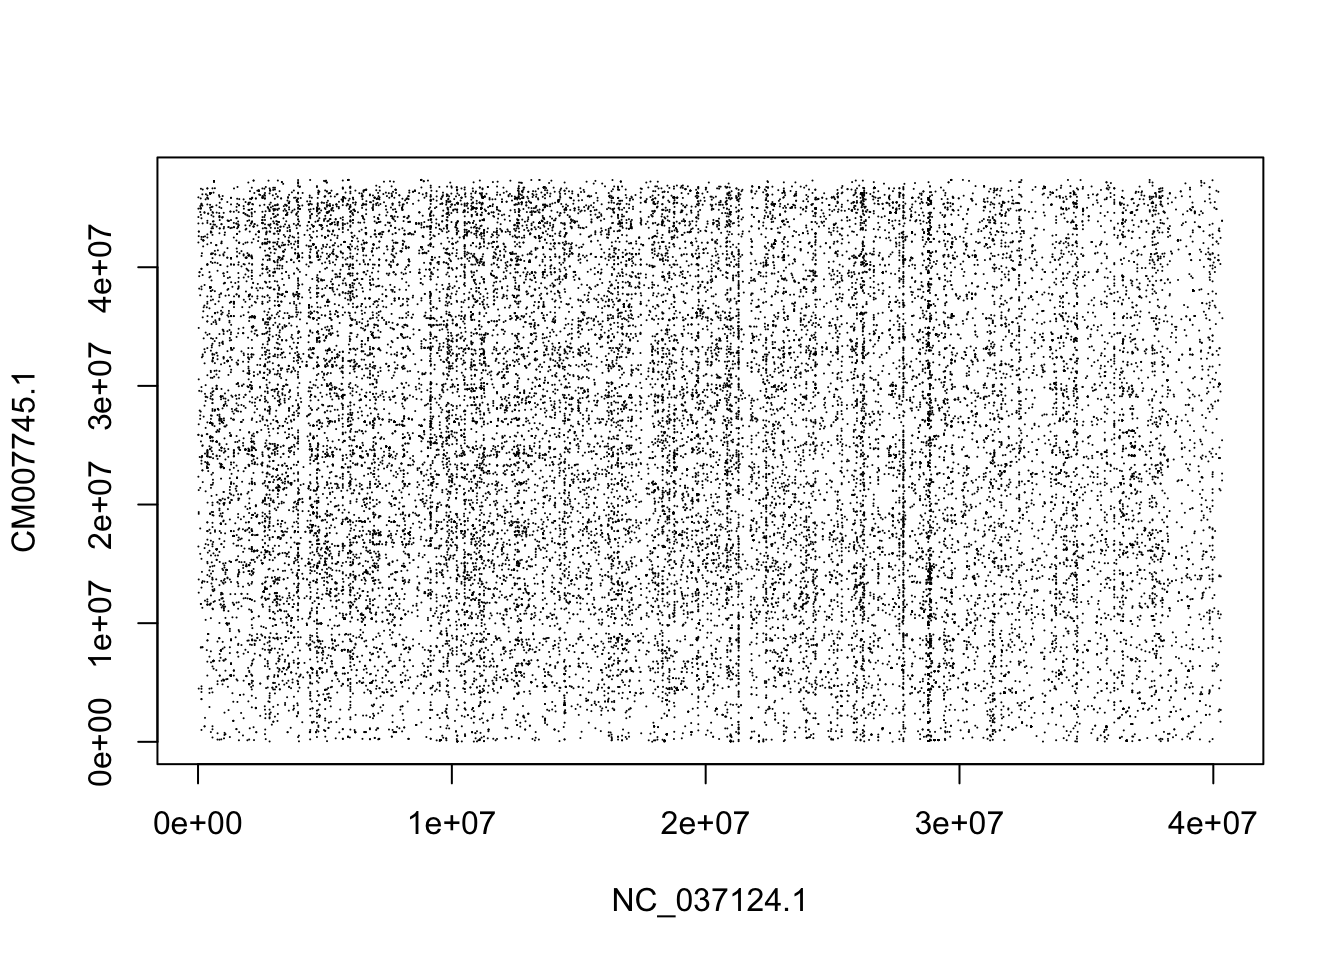
\includegraphics{eca-bioinf-handbook_files/figure-latex/unnamed-chunk-19-1.pdf}

OK, clearly what we have there is just a bunch of repetitive bits. I think we must not have the same chromosomes in the two species.

So, let's put LG28 in coho against the whole chinook genome. Note the use of the
bracketed ``multiple'' in there to let it know that there are multiple sequences in there
that should get catenated together.

\begin{Shaded}
\begin{Highlighting}[]
\BuiltInTok{time}\NormalTok{ lastz ~/Documents/UnsyncedData/Otsh_v1.0/Otsh_v1.0_genomic.fna[multiple]  coho-28.fna --notransition --step=20 --nogapped --ambiguous=iupac --format=maf }\OperatorTok{>}\NormalTok{ chin_vs_coho28.maf}

\ExtensionTok{FAILURE}\NormalTok{: in load_fasta_sequence for /Users/eriq/Documents/UnsyncedData/Otsh_v1.0/Otsh_v1.0_genomic.fna, sequence length 2,147,437,804+64,310 exceeds maximum (2,147,483,637)}
\end{Highlighting}
\end{Shaded}

No love there. But that chinook genome has a lot of short scaffolds in there too, I think.

Maybe we could just try LG1. Nope. How about we toss every coho LG against LG1 from chinook\ldots{}

\begin{Shaded}
\begin{Highlighting}[]
\CommentTok{# let's get the first 10 linkage groups from coho:}
\KeywordTok{for} \ExtensionTok{i}\NormalTok{ in }\DataTypeTok{\{1..10\}}\KeywordTok{;} \KeywordTok{do} \ExtensionTok{curl}\NormalTok{ ftp://ftp.ncbi.nlm.nih.gov/genomes/all/GCA/002/021/735/GCA_002021735.1_Okis_V1/GCA_002021735.1_Okis_V1_assembly_structure/Primary_Assembly/assembled_chromosomes/FASTA/chrLG}\VariableTok{$\{i\}}\NormalTok{.fna.gz -o coho-}\VariableTok{$\{i\}}\NormalTok{.fna.gz}\KeywordTok{;} \FunctionTok{gunzip}\NormalTok{ coho-}\VariableTok{$\{i\}}\NormalTok{.fna.gz}\KeywordTok{;} \BuiltInTok{echo} \VariableTok{$i}\KeywordTok{;} \KeywordTok{done} 

\CommentTok{# now lets try aligning those to the chinook}
\KeywordTok{for} \ExtensionTok{i}\NormalTok{ in }\DataTypeTok{\{1..10\}}\KeywordTok{;} \KeywordTok{do} \BuiltInTok{time}\NormalTok{ lastz chinook-1.fna coho-}\VariableTok{$\{i\}}\NormalTok{.fna --notransition --step=20 --nogapped --ambiguous=iupac --format=rdotplot }\OperatorTok{>}\NormalTok{ chinook1_vs_coho}\VariableTok{$\{i\}}\NormalTok{.rdp}\KeywordTok{;} \BuiltInTok{echo} \StringTok{"Done with }\VariableTok{$i}\StringTok{"}\KeywordTok{;} \KeywordTok{done}
\end{Highlighting}
\end{Shaded}

Nothing looked good until I got to coho LG10:

\begin{Shaded}
\begin{Highlighting}[]
\NormalTok{dots <-}\StringTok{ }\NormalTok{readr}\OperatorTok{::}\KeywordTok{read_tsv}\NormalTok{(}\StringTok{"inputs/chinook1_vs_coho10.rdp.gz"}\NormalTok{)}

\KeywordTok{plot}\NormalTok{(dots,}\DataTypeTok{type=}\StringTok{"l"}\NormalTok{)}
\end{Highlighting}
\end{Shaded}

There is clearly a big section that aligns there. But, we clearly are going to need to
clean up all the repetive crap, etc on these alignments.

\hypertarget{try-on-the-chinook-chromosomes}{%
\subsection{Try on the chinook chromosomes}\label{try-on-the-chinook-chromosomes}}

So, it crapped out on the full Chinook fasta. Note that I could modify the code (or compile it with a \texttt{-D}): check this out in sequences.h:

\begin{Shaded}
\begin{Highlighting}[]
\CommentTok{//  Sequence lengths are normally assumed to be small enough to fit into a}
\CommentTok{//  31-bit integer.  This gives a maximum length of about 2.1 billion bp, which}
\CommentTok{//  is half the length of a (hypothetical) monoploid human genome.  The}
\CommentTok{//  programmer can override this at compile time by defining max_sequence_index}
\CommentTok{//  as 32 or 63.}
\end{Highlighting}
\end{Shaded}

But, for now, I think I will just go for the assembled chromosomes only:

\begin{Shaded}
\begin{Highlighting}[]
\CommentTok{# just get the well assembled chromosomes (about 1.7 Gb)}
\CommentTok{# in /tmp}
\ExtensionTok{samtools}\NormalTok{ faidx ~/Documents/UnsyncedData/Otsh_v1.0/Otsh_v1.0_genomic.fna }\VariableTok{$(}\FunctionTok{awk} \StringTok{'/^NC/ \{printf("%s ", $1)\}'}\NormalTok{  ~/Documents/UnsyncedData/Otsh_v1.0/Otsh_v1.0_genomic.fna.fai}\VariableTok{)} \OperatorTok{>}\NormalTok{ chinook_nc_chroms.fna}

\CommentTok{# then try tossing coho 1 against that:}
\BuiltInTok{time}\NormalTok{ lastz chinook_nc_chroms.fna[multiple]  coho-1.fna --notransition --step=20 --nogapped --ambiguous=iupac --format=rdotplot }\OperatorTok{>}\NormalTok{ chin_nc_vs_coho1.rdp}

\CommentTok{# that took about 7 minutes}
\ExtensionTok{real}\NormalTok{    6m33.411s}
\ExtensionTok{user}\NormalTok{    6m28.391s}
\ExtensionTok{sys}\NormalTok{ 0m4.121s}
\end{Highlighting}
\end{Shaded}

Here is what the figure looks like. It is clear that the bulk of Chromosome 1
in coho aligns for long distances to two different chromosomes in Chinoook (likely
paralogs?). This is complex!

\begin{figure}
\centering
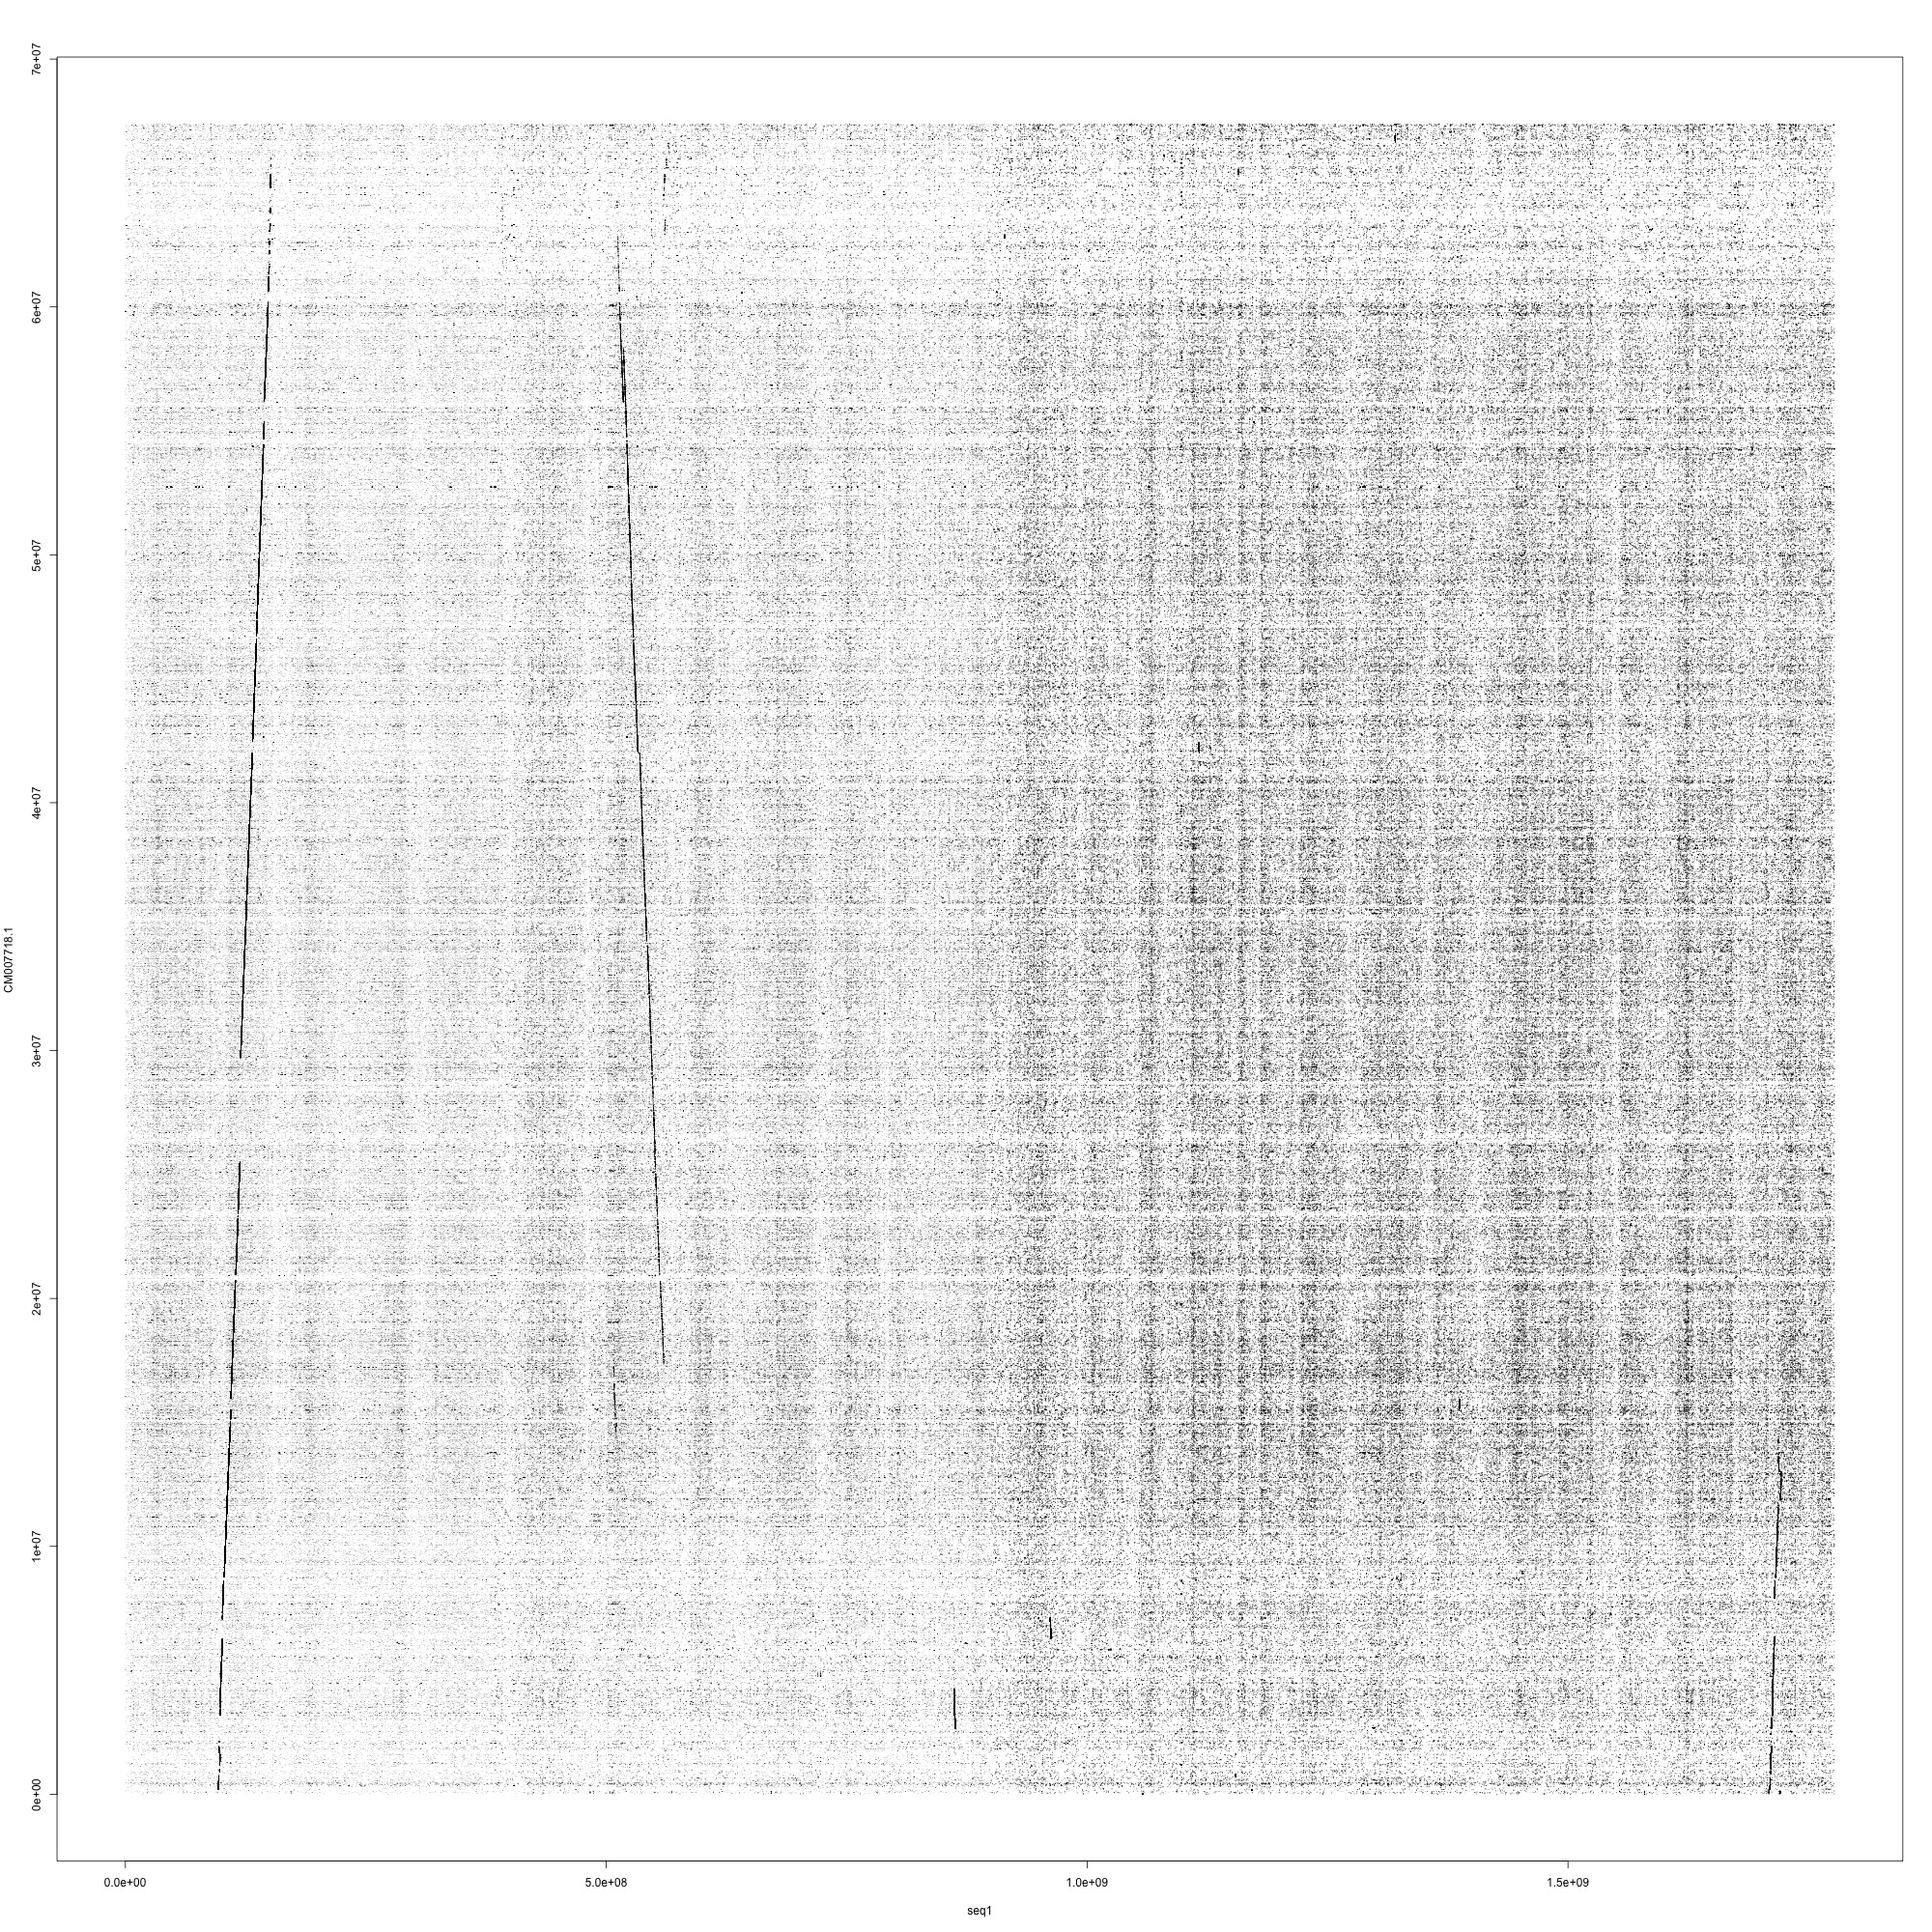
\includegraphics{figs/quickie.jpg}
\caption{Coho Chromo 1 on catenated chinook chromos}
\end{figure}

\hypertarget{explore-the-other-parameters-more}{%
\subsection{Explore the other parameters more}\label{explore-the-other-parameters-more}}

I am going to use the chinook chromosome 1 and coho 10 to explore things that will
clean up the results a little bit.

\begin{Shaded}
\begin{Highlighting}[]
\CommentTok{# in /tmp}
 \VariableTok{i=}\NormalTok{10; }\BuiltInTok{time}\NormalTok{ lastz chinook-1.fna coho-}\VariableTok{$\{i\}}\NormalTok{.fna --notransition --step=20 --nogapped --ambiguous=iupac --format=rdotplot }\OperatorTok{>}\NormalTok{ chinook1_vs_coho}\VariableTok{$\{i\}}\NormalTok{.rdp}\KeywordTok{;}
\ExtensionTok{real}\NormalTok{    0m29.055s}
\ExtensionTok{user}\NormalTok{    0m28.497s}
\ExtensionTok{sys}\NormalTok{ 0m0.413s}
\end{Highlighting}
\end{Shaded}

That is quick enough to explore a few things. Note that we are already doing gap-free extension, because
``By default seeds are extended to HSPs using x-drop extension, with entropy adjustment.'' However, by
default, chaining is not done, and that is the key step in which a path is found through the
high-scoring pairs (HSPs). That doesn't take much (any) extra time and totally cleans things up.

\begin{Shaded}
\begin{Highlighting}[]
\VariableTok{i=}\NormalTok{10; }\BuiltInTok{time}\NormalTok{ lastz chinook-1.fna coho-}\VariableTok{$\{i\}}\NormalTok{.fna --notransition --step=20 --nogapped --ambiguous=iupac --format=rdotplot --chain  }\OperatorTok{>}\NormalTok{ chinook1_vs_coho}\VariableTok{$\{i\}}\NormalTok{.rdp}\KeywordTok{;}

\ExtensionTok{real}\NormalTok{    0m28.704s}
\end{Highlighting}
\end{Shaded}

So, that is greatly improved:

\begin{Shaded}
\begin{Highlighting}[]
\NormalTok{dots <-}\StringTok{ }\NormalTok{readr}\OperatorTok{::}\KeywordTok{read_tsv}\NormalTok{(}\StringTok{"inputs/chain-chinook1_vs_coho10.rdp.gz"}\NormalTok{)}

\KeywordTok{plot}\NormalTok{(dots,}\DataTypeTok{type=}\StringTok{"l"}\NormalTok{)}
\end{Highlighting}
\end{Shaded}

So, it would be worth seeing if chaining also cleans up the multi-chrom alignment:

\begin{Shaded}
\begin{Highlighting}[]
\BuiltInTok{time}\NormalTok{ lastz chinook_nc_chroms.fna[multiple]  coho-1.fna --notransition --step=20 --nogapped --ambiguous=iupac --format=rdotplot --chain }\OperatorTok{>}\NormalTok{ chin_nc_vs_coho1.rdp}

\ExtensionTok{real}\NormalTok{    6m42.835s}
\ExtensionTok{user}\NormalTok{    6m35.042s}
\ExtensionTok{sys}\NormalTok{ 0m6.207s}
\end{Highlighting}
\end{Shaded}

\begin{Shaded}
\begin{Highlighting}[]
\NormalTok{dots <-}\StringTok{ }\NormalTok{readr}\OperatorTok{::}\KeywordTok{read_tsv}\NormalTok{(}\StringTok{"inputs/chin_nc_vs_coho1-chain.rdp.gz"}\NormalTok{)}

\KeywordTok{plot}\NormalTok{(dots,}\DataTypeTok{type=}\StringTok{"l"}\NormalTok{)}
\end{Highlighting}
\end{Shaded}

OK, that shows that it will find crappy chains if given the chance. But if you
zoom in on that stuff you see that some of the spots are pretty short, and some are super
robust. So, we will want some further filtering
to make this work. So, we need to check out the ``back-end filtering.'' that is possible.
Back-end filtering does not happen by default.

Let's say that we want 70 Kb alignment blocks. That is .001 of the total input sequence.

\begin{Shaded}
\begin{Highlighting}[]
\BuiltInTok{time}\NormalTok{ lastz chinook_nc_chroms.fna[multiple]  coho-1.fna --notransition --step=20 --nogapped --ambiguous=iupac --format=rdotplot --chain --coverage=0.1 }\OperatorTok{>}\NormalTok{ chin_nc_vs_coho1-cov-0.1.rdp}
\end{Highlighting}
\end{Shaded}

That took 6.5 minutes again. But, it also produced no output whatsoever. We probably
want to filter on identity first anyway. Because that takes so long, maybe we could
do it with our single chromosome first.

\begin{Shaded}
\begin{Highlighting}[]
\VariableTok{i=}\NormalTok{10; }\BuiltInTok{time}\NormalTok{ lastz chinook-1.fna coho-}\VariableTok{$\{i\}}\NormalTok{.fna --notransition --step=20 --nogapped --ambiguous=iupac --format=rdotplot --chain  }\OperatorTok{>}\NormalTok{ chinook1_vs_coho}\VariableTok{$\{i\}}\NormalTok{.rdp}\KeywordTok{;}
\end{Highlighting}
\end{Shaded}

\begin{Shaded}
\begin{Highlighting}[]
\NormalTok{dots <-}\StringTok{ }\NormalTok{readr}\OperatorTok{::}\KeywordTok{read_tsv}\NormalTok{(}\StringTok{"/tmp/chinook1_vs_coho10-ident95.rdp"}\NormalTok{)}

\KeywordTok{plot}\NormalTok{(dots,}\DataTypeTok{type=}\StringTok{"l"}\NormalTok{)}
\end{Highlighting}
\end{Shaded}

That keeps things very clean, but the alignment blocks are all pretty short (like 50 to 300
bp long). So perhaps we need to do gapped extension here to make these things better. This
turns out to take a good deal longer.

\begin{Shaded}
\begin{Highlighting}[]
\VariableTok{i=}\NormalTok{10; }\BuiltInTok{time}\NormalTok{ lastz chinook-1.fna coho-}\VariableTok{$\{i\}}\NormalTok{.fna --notransition --step=20 --gapped --ambiguous=iupac --format=maf --chain --identity=95  }\OperatorTok{>}\NormalTok{ chinook1_vs_coho}\VariableTok{$\{i\}}\NormalTok{-ident95-gapped.maf}\KeywordTok{;}

\ExtensionTok{real}\NormalTok{    3m15.575s}
\ExtensionTok{user}\NormalTok{    3m14.048s}
\ExtensionTok{sys}\NormalTok{ 0m0.936s}
\end{Highlighting}
\end{Shaded}

\begin{Shaded}
\begin{Highlighting}[]
\NormalTok{dots <-}\StringTok{ }\NormalTok{readr}\OperatorTok{::}\KeywordTok{read_tsv}\NormalTok{(}\StringTok{"/tmp/chinook1_vs_coho10-ident95-gapped.rdp"}\NormalTok{)}
\KeywordTok{plot}\NormalTok{(dots,}\DataTypeTok{type=}\StringTok{"l"}\NormalTok{)}
\end{Highlighting}
\end{Shaded}

That is pretty clean and slick.

Now, this has got me to thinking that maybe I \emph{can} do this on a chromosome by chromosome basis.

Check what 97\% identity looks like:

\begin{Shaded}
\begin{Highlighting}[]
\VariableTok{i=}\NormalTok{10; }\BuiltInTok{time}\NormalTok{ lastz chinook-1.fna coho-}\VariableTok{$\{i\}}\NormalTok{.fna --notransition --step=20 --gapped --ambiguous=iupac --format=rdotplot --chain --identity=97  }\OperatorTok{>}\NormalTok{ chinook1_vs_coho}\VariableTok{$\{i\}}\NormalTok{-ident97-gapped.rdp}\KeywordTok{;}
\end{Highlighting}
\end{Shaded}

\begin{Shaded}
\begin{Highlighting}[]
\NormalTok{dots <-}\StringTok{ }\NormalTok{readr}\OperatorTok{::}\KeywordTok{read_tsv}\NormalTok{(}\StringTok{"/tmp/chinook1_vs_coho10-ident97-gapped.rdp"}\NormalTok{)}
\KeywordTok{plot}\NormalTok{(dots,}\DataTypeTok{type=}\StringTok{"l"}\NormalTok{)}
\end{Highlighting}
\end{Shaded}

That looks to have a few more holes in it.

Final test. Let's see what happens when we chain it on a chromosome that doesn't have
any homology:

\begin{Shaded}
\begin{Highlighting}[]
\CommentTok{# first with no backend filtering}
\VariableTok{i=}\NormalTok{1; }\BuiltInTok{time}\NormalTok{ lastz chinook-1.fna coho-}\VariableTok{$\{i\}}\NormalTok{.fna --notransition --step=20 --gapped --ambiguous=iupac --format=rdotplot --chain  }\OperatorTok{>}\NormalTok{ chinook1_vs_coho}\VariableTok{$\{i\}}\NormalTok{-gapped.rdp}\KeywordTok{;}

\ExtensionTok{real}\NormalTok{    0m35.130s}
\ExtensionTok{user}\NormalTok{    0m34.642s}
\ExtensionTok{sys}\NormalTok{ 0m0.413s}

\CommentTok{# Hey! That is cool.  When there are no HSPs to chain, this doesn't take very long}
\VariableTok{i=}\NormalTok{1; }\BuiltInTok{time}\NormalTok{ lastz chinook-1.fna coho-}\VariableTok{$\{i\}}\NormalTok{.fna --notransition --step=20 --gapped --ambiguous=iupac --format=rdotplot --chain --identity=95 }\OperatorTok{>}\NormalTok{ chinook1_vs_coho}\VariableTok{$\{i\}}\NormalTok{-gapped-ident95.rdp}\KeywordTok{;}
\end{Highlighting}
\end{Shaded}

\begin{Shaded}
\begin{Highlighting}[]
\NormalTok{dots <-}\StringTok{ }\NormalTok{readr}\OperatorTok{::}\KeywordTok{read_tsv}\NormalTok{(}\StringTok{"/tmp/chinook1_vs_coho1-gapped.rdp"}\NormalTok{)}
\KeywordTok{plot}\NormalTok{(dots,}\DataTypeTok{type=}\StringTok{"l"}\NormalTok{)}
\end{Highlighting}
\end{Shaded}

OK, it finds something nice and crappy there.

What about if we require 95\% identity?

\begin{Shaded}
\begin{Highlighting}[]
\NormalTok{dots <-}\StringTok{ }\NormalTok{readr}\OperatorTok{::}\KeywordTok{read_tsv}\NormalTok{(}\StringTok{"/tmp/chinook1_vs_coho1-gapped-ident95.rdp"}\NormalTok{)}
\KeywordTok{plot}\NormalTok{(dots,}\DataTypeTok{type=}\StringTok{"l"}\NormalTok{)}
\end{Highlighting}
\end{Shaded}

That leaves us with very little.

Let's also try interpolation at the end to see how that does. Note that here we also produce the
rdotplot at the same time as the maf.

\begin{Shaded}
\begin{Highlighting}[]
\VariableTok{i=}\NormalTok{10; }\BuiltInTok{time}\NormalTok{ lastz chinook-1.fna coho-}\VariableTok{$\{i\}}\NormalTok{.fna --notransition --step=20 --gapped --ambiguous=iupac --format=maf --rdotplot=chinook1_vs_coho}\VariableTok{$\{i\}}\NormalTok{-ident95-gapped-inner1000.rdp --chain --identity=95 --inner=1000 }\OperatorTok{>}\NormalTok{ chinook1_vs_coho}\VariableTok{$\{i\}}\NormalTok{-ident95-gapped-inner1000.maf}\KeywordTok{;}

\ExtensionTok{real}\NormalTok{    4m25.625s}
\ExtensionTok{user}\NormalTok{    4m22.957s}
\ExtensionTok{sys}\NormalTok{ 0m1.478s}
\end{Highlighting}
\end{Shaded}

That took an extra minute, but was not so bad.

\begin{Shaded}
\begin{Highlighting}[]
\NormalTok{dots <-}\StringTok{ }\NormalTok{readr}\OperatorTok{::}\KeywordTok{read_tsv}\NormalTok{(}\StringTok{"/tmp/chinook1_vs_coho10-ident95-gapped-inner1000.rdp"}\NormalTok{)}
\KeywordTok{plot}\NormalTok{(dots,}\DataTypeTok{type=}\StringTok{"l"}\NormalTok{)}
\end{Highlighting}
\end{Shaded}

\hypertarget{repeat-masking-the-coho-genome}{%
\subsubsection{Repeat Masking the Coho genome}\label{repeat-masking-the-coho-genome}}

Turns out that NCBI site has the repeat masker output in GCF\_002021735.1\_Okis\_V1\_rm.out.gz.
I save that to a shorter name. Now I will make a bed file of the repeat regions. Then I use bedtools maskfasta to softmask that fasta file.

\begin{Shaded}
\begin{Highlighting}[]
\CommentTok{# in: /Users/eriq/Documents/UnsyncedData/Okis_v1}
\ExtensionTok{gzcat}\NormalTok{ Okis_V1_rm.out.gz }\KeywordTok{|} \FunctionTok{awk} \StringTok{'NR>3 \{printf("%s\textbackslash{}t%s\textbackslash{}t%s\textbackslash{}n", $5, $6, $7)\}'} \OperatorTok{>}\NormalTok{ repeat-regions.bed }

\ExtensionTok{bedtools}\NormalTok{ maskfasta -fi Okis_V1.fna -bed repeat-regions.bed  -fo Okis_V1-soft-masked.fna  -soft}
\end{Highlighting}
\end{Shaded}

That works great. But it turns out that the coho genome is already softmasked.

But, it is good to now that I can use a repeat mask output file to toss repeat
sites if I want to for ANGSD analyses, etc.

\hypertarget{multiz-maf2fasta}{%
\subsubsection{multiz maf2fasta}\label{multiz-maf2fasta}}

So, it looks like you can use single\_cov2 from multiz to retain only a single
alignment block covering each area. Then you can maf2fasta that and send it off in
fasta format. Line2 holds the reference (target) sequence, but it has dashes added where
the query has stuff not appearing in the target. So, what you have to do is run through that sequence and drop all the positions in the query that correspond to dashes in the
target. That will get us what we want.

But maybe I can just use megablast like Christensen and company. They have some of their
scripts, but it is not clear to me that it will be easy to get that back to a fasta
for later analysis in ANGSD.

Not only that, but then there is the whole paralog issue. I am exploring that a little
bit right now. It looks like when you crank the identity requirement up, the paralogs
get pretty spotty so they can be easily recognized. For example setting the identity
at 99.5 makes it clear which is the paralog:

\begin{Shaded}
\begin{Highlighting}[]
\BuiltInTok{time}\NormalTok{ lastz chinook_nc_chroms.fna[multiple]  coho-1.fna --notransition --step=20 --nogapped --ambiguous=iupac --format=rdotplot --chain --identity=99.5 }\OperatorTok{>}\NormalTok{ chin_nc_vs_coho1-chain-ident-99.5.rdp}
\CommentTok{# takes about 6 minutes}
\end{Highlighting}
\end{Shaded}

And the figure is here.

\begin{figure}
\centering
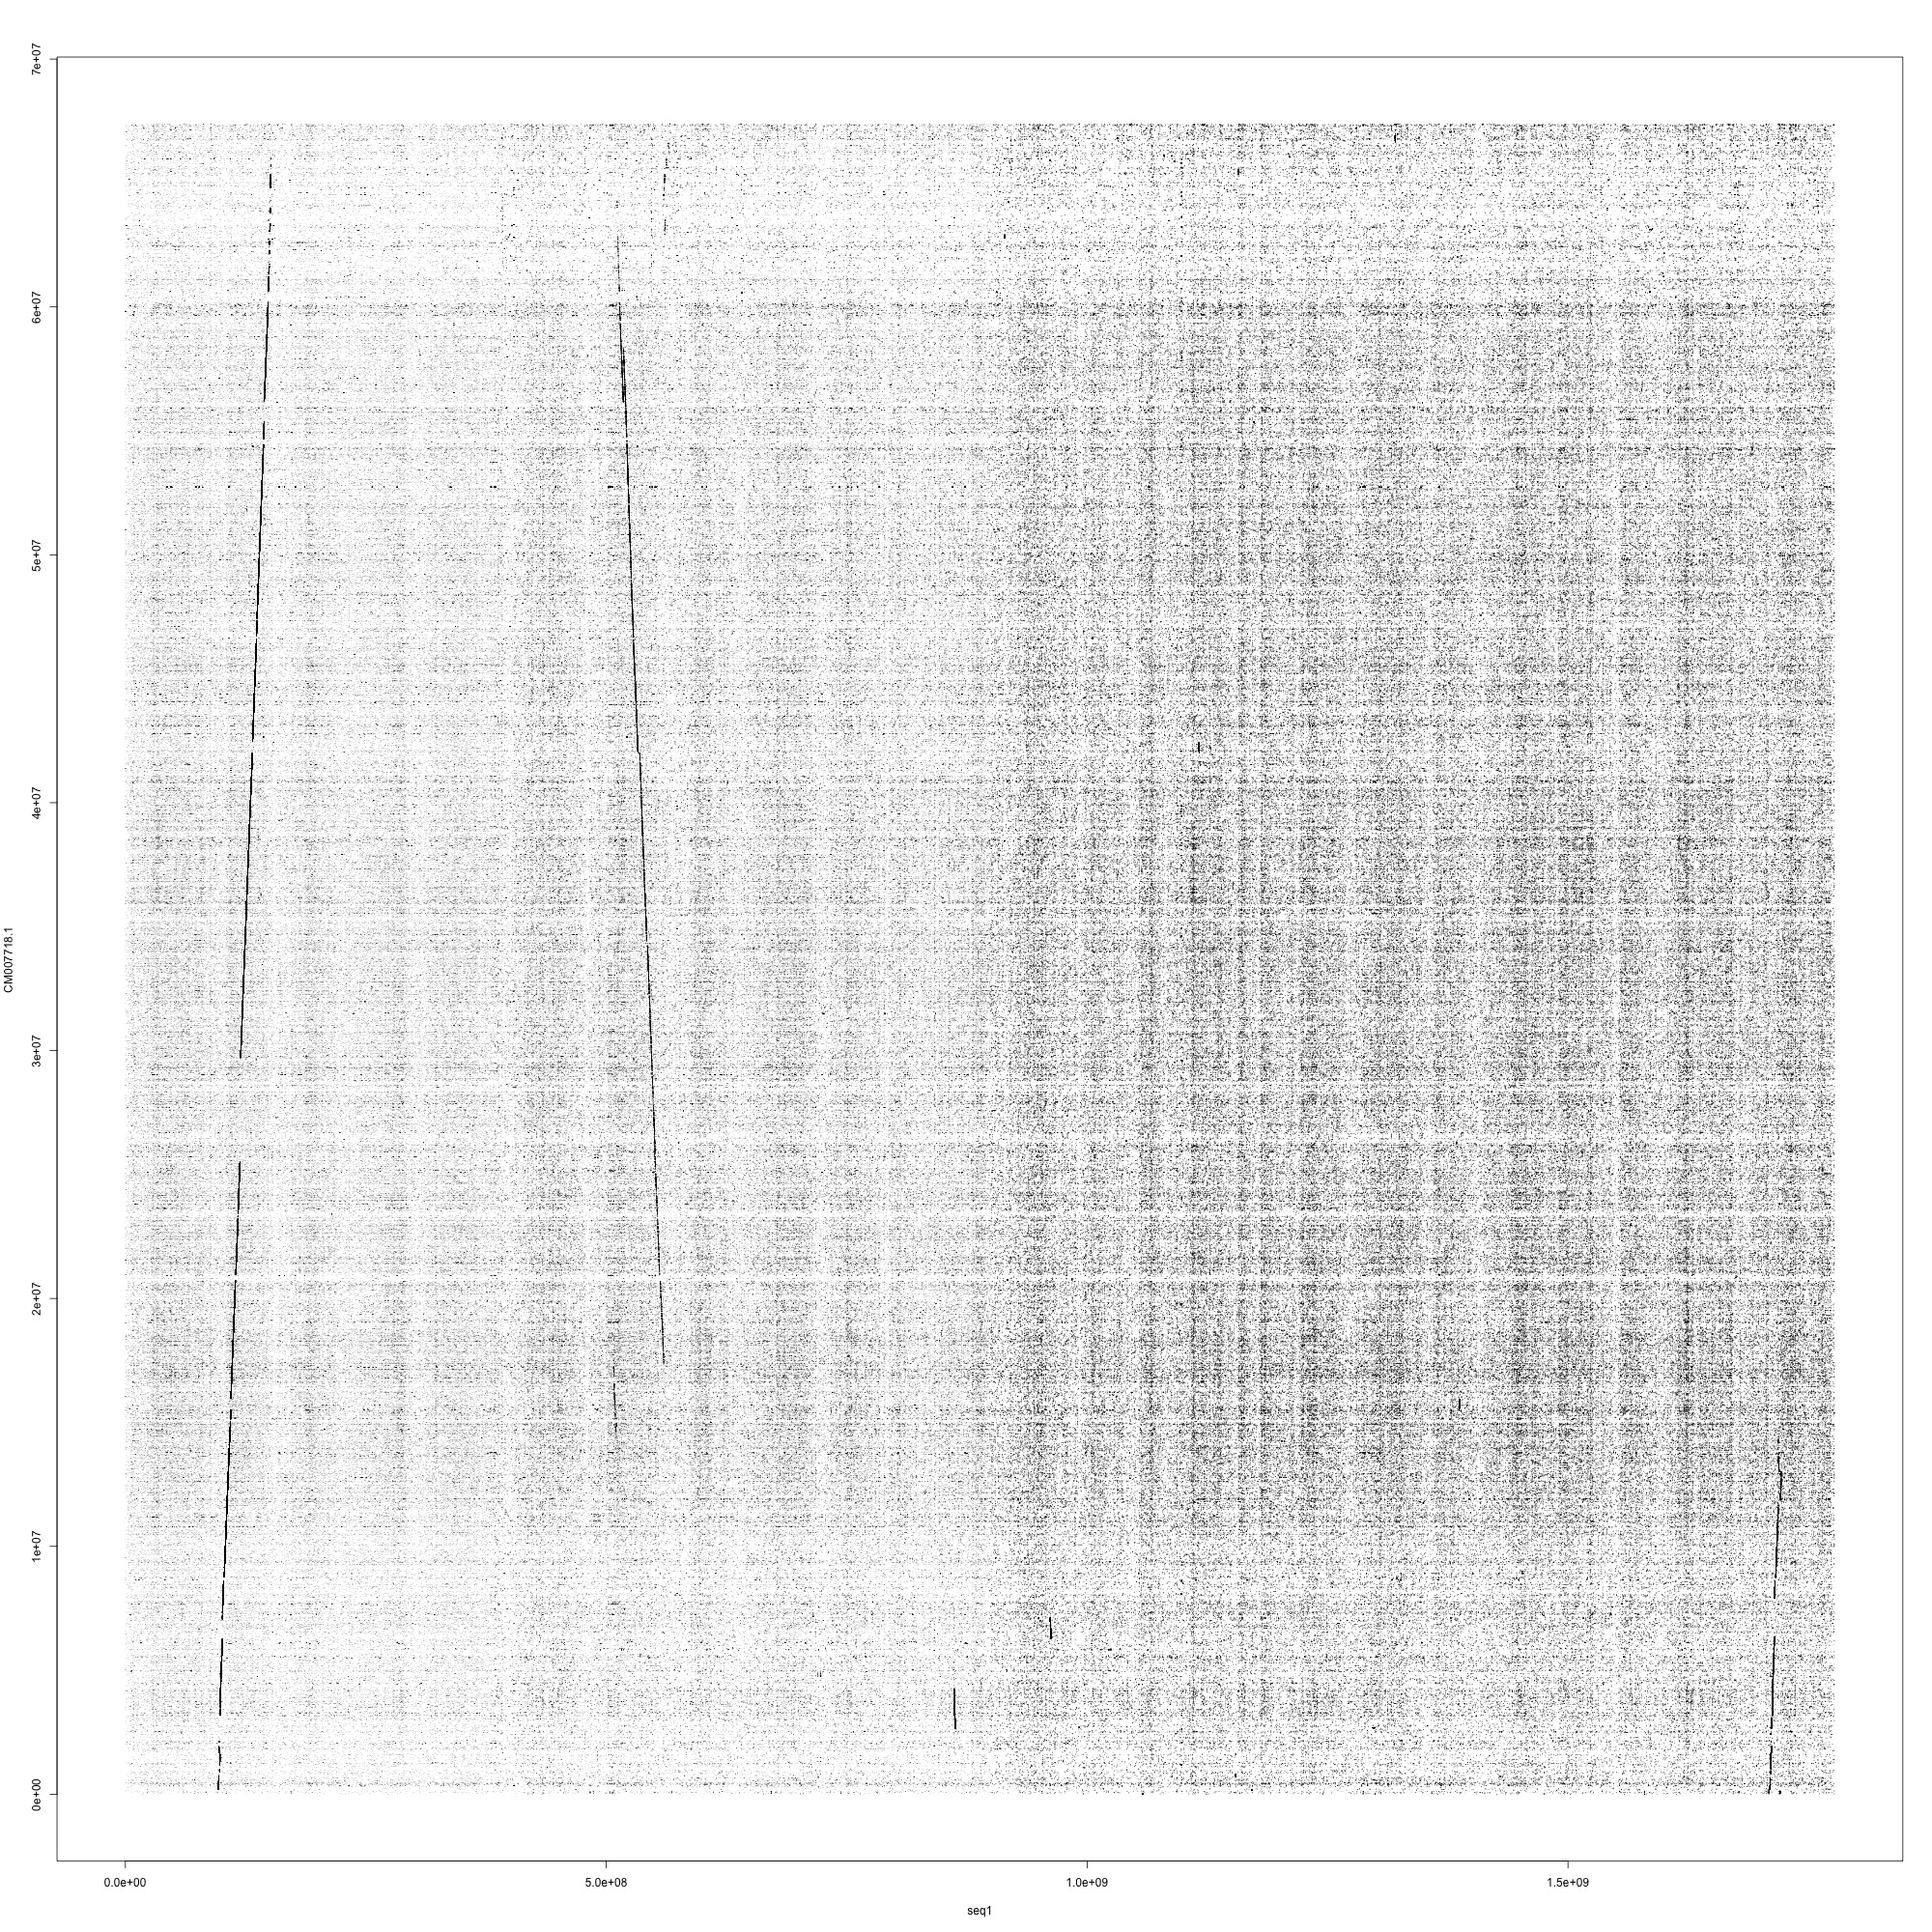
\includegraphics{figs/quickie.jpg}
\caption{Coho Chromo 1 on catenated chinook chromos. Ident=99.5}
\end{figure}

So, I think this is going to be a decent workflow:

\begin{enumerate}
\def\labelenumi{\arabic{enumi}.}
\tightlist
\item
  run lastz on each coho linkage group against each chinook chromosome separately. Do this at identity=92 and identity=95 and identity=99.9. For each run, produce a .maf file and
  at the same time a .rdotplot output.
\item
  Combine all the .rdotplot files together into something that can be faceted over
  chromosomes and make a massive facet grid showing the results for all chromosomes.
  Do this at different identity levels so that the paralogs can be distinguished.
\item
  Visually look up each columns of those plots and determine which coho chromosomes
  carry homologous material for each chinook chromosome. For each such chromosome pair,
  run single\_cov2 on them (maybe on the ident=92 version).
\item
  Then merge those MAFs. Probably can just cat them together, but there might be some
  sorting that needs to be done on them.
\item
  Run maf2fasta on those merged mafs to get a fasta for each chinook chromosome.
\item
  Write a C-program that uses uthash to efficiently read the fasta for each chinook
  chromosome and then write out a version in which the positions that are dashes in the
  chinook reference are removed from both the chinook reference and the aligned coho
  sequence. \_Actually, one can just pump each sequence out to a separate file in which
  each site occupies one line. Then paste those and do the comparison\ldots{}
\end{enumerate}

\begin{Shaded}
\begin{Highlighting}[]
\ExtensionTok{2018-10-18}\NormalTok{ 11:15 /tmp/--% time (awk }\StringTok{'NR==2'}\NormalTok{ splud }\KeywordTok{|} \ExtensionTok{fold}\NormalTok{ -w1 }\OperatorTok{>}\NormalTok{ spp1.text)}

\ExtensionTok{real}\NormalTok{    0m23.244s}
\ExtensionTok{user}\NormalTok{    0m22.537s}
\ExtensionTok{sys}\NormalTok{ 0m0.685s}

\CommentTok{# then you can use awk easily like this:}
\ExtensionTok{paste}\NormalTok{ spp1.text spp2.text }\KeywordTok{|} \FunctionTok{awk} \StringTok{'BEGIN \{SUBSEP = " "\} \{n[$1,$2]++\} END \{for(i in n) print i, n[i]\}'} 
\end{Highlighting}
\end{Shaded}

\begin{enumerate}
\def\labelenumi{\arabic{enumi}.}
\setcounter{enumi}{6}
\tightlist
\item
  The coho sequence thus obtained will have dashes anywhere there isn't coho aligned
  to the chinook. So, first, for each chromosome I can count the number of dashes, which
  will tell me the fraction of sites on the chinook genome that were aligned (sort of---there is an issue with N's in the coho genome.) Then those dashes can be converted to N's.
\item
  It would be good to count the number of sites that are not N's in chinook that are also
  not Ns in coho, to know how much of it we have aligned.
\end{enumerate}

Note, the last thing that really remains here is making sure that I can run two or more different query sequences against one chinook genome and then process that out correctly
into a fasta.

Note that Figure 1 in christensen actually gives me a lot to go on in terms of which
chromosomes in coho to map against which ones in chinook.

\hypertarget{part-part-iv-analysis-of-big-variant-data}{%
\part{Part IV: Analysis of Big Variant Data}\label{part-part-iv-analysis-of-big-variant-data}}

\hypertarget{bioinformatic-analysis-on-variant-data}{%
\chapter{Bioinformatic analysis on variant data}\label{bioinformatic-analysis-on-variant-data}}

Standard analyses like computing Fst and linkage disequilibrium, etc., from
data, typically in a VCF file.

Basically, we want to get comfortable with plink 2.0, bedtools, vcftools, etc.

The key in all of this is to motivate every single thing we do here in terms of an
application in conservation genomics. That is going to be key.

This Part IV will be about standard bioinformatic tools for doing things
with big variant data.

\begin{itemize}
\tightlist
\item
  Filtering
\item
  Imputation
\item
  LD, HWD, FST
\item
  Etc.
\end{itemize}

I will probably have a chapter on unix tools.

Maybe another on R/Bioconductor tools.

Gotta have a chapter about ``Look at your data!'' and Whoa! and diagnostics
using radiator.

\hypertarget{part-part-v-population-genomics}{%
\part{Part V: Population Genomics}\label{part-part-v-population-genomics}}

\hypertarget{topics-in-pop-gen}{%
\chapter{Topics in pop gen}\label{topics-in-pop-gen}}

This is just a bunch of ideas. But basically, I want to have some topics here that
everyone should know about. Slanted toward things that are relevant for inference
or simulation.

\hypertarget{coalescent}{%
\section{Coalescent}\label{coalescent}}

Gotta have a lecture on the coalescent. It would be nice to try to motivate
all the topics from this backward in time perspective.

Get far enough to discuss \(\pi\) and the expected site frequency spectrum.

\hypertarget{measures-of-genetic-diversity-and-such}{%
\section{Measures of genetic diversity and such}\label{measures-of-genetic-diversity-and-such}}

It would really be good for me to write a chapter / give a few lectures
on different measures like dxy and fst

From Ash's paper: However, population genomic analyses (outlined below) use FST only, as dxy was highly correlated to nucleotide diversity (for early stage diverging populations the correlation between dxy and \(\pi\) is \textgreater{} 0.91, Pearson correlation). As such variation in dxy across the genome reflects variation in diversity, not differentiation (Riesch et al., 2017).

Tajima's \(D\) and such. The influence of selection on such measures.

\hypertarget{demographic-inference-with-partial-a-partial-i-and-moments}{%
\section{\texorpdfstring{Demographic inference with \(\partial a \partial i\) and \emph{moments}}{Demographic inference with \textbackslash{}partial a \textbackslash{}partial i and moments}}\label{demographic-inference-with-partial-a-partial-i-and-moments}}

\hypertarget{balls-in-boxes}{%
\section{Balls in Boxes}\label{balls-in-boxes}}

Would be worthwhile to have a review of all these sorts of variants of
population assignment, structure, admixture, etc.

Population structure and PCAs.

finestructure and fineRADstructure.

Might want to insert \citet{BradburdInferringContinuousDiscrete2018}.

Might also want to discuss \citet{PickrellInferencePopulationSplits2012}.

Also: \citet{PritchardInferencePopulationStructure2000}

What if we go and try to put the same one in? Like Pritch 2000 again: \citep{PritchardInferencePopulationStructure2000}

\hypertarget{some-landscape-genetics}{%
\section{Some landscape genetics}\label{some-landscape-genetics}}

After talking with Amanda about her dissertation I realized it would be good
to talk about some landscape genetics stuff. For sure I want to talk about
EEMS and maybe CircuitScape, just so I know well what is going on with the
latter.

\hypertarget{relationship-inference}{%
\section{Relationship Inference}\label{relationship-inference}}

Maybe do a lecture on this\ldots{}

\hypertarget{tests-for-selection}{%
\section{Tests for Selection}\label{tests-for-selection}}

A look at a selection of the methods that are out there. FST outliers, \emph{Bayescan}, \emph{Lositan}, \emph{PCAdapt}, and friends. It would be good to get a nice succinct explanation/understanding of all of these.

\hypertarget{multivariate-associations-gea-etc.}{%
\section{Multivariate Associations, GEA, etc.}\label{multivariate-associations-gea-etc.}}

It really is time for me to wrap my head around this stuff.

\hypertarget{estimating-heritability-in-the-wild}{%
\section{Estimating heritability in the wild}\label{estimating-heritability-in-the-wild}}

Another from Amanda. It would be good to do some light Quant Genet so that
we all understand how we might be able to use NGS data to estimate heritability
in wild populations.

\bibliography{references.bib,book.bib}

\backmatter
\printindex

\end{document}
